%% PhD Thesis Template for City University London.
%% Ciro Moreno Ramírez
%% July 2015


%%Document type: book
%%
%%Paper size:	A4	(compulsory)
%%
%%Font size: 	11p	(minimun allowed: 8p)
%%
%%Line spacing:	1.5x	(1.5x or 2x allowed)
%%
%%Page margins:	inner  =   4cm, (minimum allowed: 4cm)
%%				outer  =   3cm,	(minimum allowed: 2cm)
%%				top    = 2.5cm,	(minimum allowed: 2cm)
%%				bottom =   3cm	(minimum allowed: 2cm)


% --- Preamble --- %

%% Document definition:
\documentclass[11pt,a4paper,twoside,openright]{book}
\pagestyle{plain}

%Page geometry:
\usepackage[inner=4cm, outer=3cm, top=2.5cm, bottom=3cm]{geometry}

%Distance from the page number to the botom edge:
\setlength{\footskip}{1.5cm}

%Line spacing:
\renewcommand{\baselinestretch}{1.5}


%User's packages
%This is the part of the preface in which the used packages are defined.

% *** LINE SPACING
\usepackage{setspace}
%\spacing{1.5}

% *** CAPTION
\usepackage{caption}
\captionsetup{margin=10pt,font={footnotesize, singlespacing},labelfont=bf,justification=justified}

% *** CITATION PACKAGES ***

%\usepackage{natbib}
\usepackage{natbib,har2nat} %har2nat to use the harvard bibliography style

%%% Multiple Bibliographies: To introduce the Contribution chapter
\usepackage{multibib}
\newcites{ctb}{Contributions}
%When using multibib package on Windows it may fail to produce the extra bibliographies. The solution is to run manually the following compilations:
%pdflatex thesis.tex
%bibtex thesis.tex
%bibtex ctb.aux			-> This file is created after running the previous compilation in the thesis.tex folder
%pdflatex thesis.tex
%pdflatex thesis.tex
%Check multibib documentation for more options. - https://www.ctan.org/pkg/multibib

% *** HIPERLINKS
\usepackage[hidelinks]{hyperref}
% *** URL
\usepackage{url}
\urlstyle{same}  % tt,rm,sf,same

% *** GRAPHICS PACKAGES ***
\usepackage[pdftex]{graphicx}
\DeclareGraphicsExtensions{.png}

\usepackage{tabularx}

% *** SUBFIGURE PACKAGES ***
\usepackage[caption=false,font=scriptsize,position=t,singlelinecheck=off]{subfig}

% *** ALIGNMENT PACKAGES ***
\usepackage{array}
\usepackage{multirow}

% *** MATH PACKAGES ***
\usepackage[cmex10]{amsmath}

%% *** MISC ***
\usepackage{makeidx} %If you want to generate an index, automatically
\usepackage{lipsum} % To generate the Loren Ipsum random text.
\usepackage{color} %To modify the color.
\usepackage{enumerate} %To modify the counter style in the enumerate environment.
\usepackage{amssymb} %Some extra symbols.
%\usepackage{listings} %To include the source code of any programming language within your document.
\usepackage{graphicx}
\usepackage{enumerate}
\usepackage{amsthm}
\usepackage{amsmath}
\usepackage{amsfonts}

\usepackage{algorithm}
\usepackage{leftindex}


%User's functions
%This is the part of the preface in which the user can define his/her functions.

%% Custom enumerate environment:
\newenvironment{packed_enum}{
\begin{enumerate}[a)]
  \setlength{\itemsep}{1pt}
  \setlength{\parskip}{0pt}
  \setlength{\parsep}{0pt}
}{\end{enumerate}}


%%Imagen 2 x root locus:
\newcommand{\tablefigs}[8]{
\begin{figure}[#8]
\centering
\begin{tabular}{cc}
\hspace{-4mm}
\subfloat[#3]{\includegraphics[width=0.5\linewidth]{#1/#2}\label{#2}}\hspace{0mm}
\subfloat[#5]{\includegraphics[width=0.5\linewidth]{#1/#4}\label{#3}}\hspace{0mm}
\end{tabular}
\caption{#6}
\label{#7}
\end{figure}}


%%%%%%%% ----------- ROTATION MATRICES ----------- %%%%%%%%

%%%%----------------- MATRIZ ROT Z -----------------%%%%
\newcommand{\zrot}[1]{
%\begin{displaymath}
\left(
\begin{array}{ccc}
\cos#1 & -\sin#1 & 0 \\
\sin#1 &  \cos#1 & 0 \\
	0 	& 	  0    & 1 \\
\end{array}
\right)
%\end{displaymath}
}
%%%%------------------------------------------------%%%%

%%%%----------------- INVERS ROT Z -----------------%%%%
\newcommand{\zroti}[1]{
%\begin{displaymath}
\left(
\begin{array}{ccc}
 \cos#1 & \sin#1 & 0 \\
-\sin#1 & \cos#1 & 0 \\
	0 	 & 	  0    & 1 \\
\end{array}
\right)
%\end{displaymath}
}
%%%%------------------------------------------------%%%%




%%%%----------------- MATRIZ ROT Y -----------------%%%%
\newcommand{\yrot}[1]{
%\begin{displaymath}
\left(
\begin{array}{ccc}
 \cos#1 & 0 & \sin#1	\\
	0	 & 1 &	0 		\\
-\sin#1 & 0 & \cos#1	\\
\end{array}
\right)
%\end{displaymath}
}
%%%%------------------------------------------------%%%%

%%%%----------------- INVERS ROT Y -----------------%%%%
\newcommand{\yroti}[1]{
%\begin{displaymath}
\left(
\begin{array}{ccc}
\cos#1 & 0 & -\sin#1	\\
	0	& 1 &	0 		\\
\sin#1 & 0 &  \cos#1	\\
\end{array}
\right)
%\end{displaymath}
}
%%%%------------------------------------------------%%%%




%%%%----------------- MATRIZ ROT X -----------------%%%%
\newcommand{\xrot}[1]{
%\begin{displaymath}
\left(
\begin{array}{ccc}
1 &	   0	&	  0 	\\
0 &	\cos#1 & -\sin#1	\\
0 &	\sin#1 &  \cos#1	\\
\end{array}
\right)
%\end{displaymath}
}
%%%%------------------------------------------------%%%%

%%%%----------------- INVERS ROT X -----------------%%%%
\newcommand{\xroti}[1]{
%\begin{displaymath}
\left(
\begin{array}{ccc}
1 &	    0	 &	  0 	\\
0 &	 \cos#1 & \sin#1	\\
0 &	-\sin#1 & \cos#1	\\
\end{array}
\right)
%\end{displaymath}
}
%%%%------------------------------------------------%%%%

\newcommand\numberthis{\addtocounter{equation}{1}\tag{\theequation}}
\newcommand\underrel[2]{\mathrel{\mathop{#2}\limits_{#1}}}
\theoremstyle{plain}
\newtheorem{theorem}{Theorem}[section]
\newtheorem{proposition}{Proposition}[section]
\newtheorem{conjecture}{Conjecture}[section]


\theoremstyle{definition}
\newtheorem{definition}{Definition}[section]

\theoremstyle{remark}
\newtheorem{remark}{Remark}[section]
\newtheorem{corollary}{Corollary}[section]





% --- Document --- %

% Including chapters individually:
%This comand avoids compiling all the thesis when working with only certain chapters.
%\includeonly{Frontmatter/Titlepage}

\begin{document}




%% Front matter ------------------------------
\frontmatter

%Title page
\begin{titlepage}
    \begin{center}
        \vspace*{2mm}
        
        %Full title of the thesis, as approved by the Board of Studies, which should describe the contents accurately and concisely
        \begin{spacing}{1.2}
        \Huge
        \textbf{Mathematical Classification of the Modes of Tumour Evolution}
 		\end{spacing}
        
        %Full name of the author
        \vspace{1cm}
        \Large
        \textbf{Veselin Manojlovi\'c}

        \vspace{1.5cm}
        
        %Qualification for which the thesis is submitted
        \begin{spacing}{1}
        Doctor of Philosophy\\
        \end{spacing}
        
        \vspace{2cm} 
		
		%City University logo
	    
\includegraphics[width=0.35\textwidth]{Frontmatter/CU_logo_S1}
	    
	    \vspace{1cm}

		%Name of the institution to which the thesis is submitted
		\textbf{School of Science and Technology}\\
		%Department or organisation in which the research was conducted
        \textbf{Department of Mathematics}\\
        
        \vfill
		%Month and year of submission
        September $2023$
        
    \end{center}
\end{titlepage}

%Table of contents
\cleardoublepage
\phantomsection
\addcontentsline{toc}{chapter}{Contents}
\tableofcontents

%List of figures
\cleardoublepage
\phantomsection
\addcontentsline{toc}{chapter}{\listfigurename}
\listoffigures

%List of tables
\cleardoublepage
\phantomsection
\addcontentsline{toc}{chapter}{\listtablename}
\listoftables

%Acknowledgements
\chapter*{Acknowledgements}
\addcontentsline{toc}{chapter}{Acknowledgements}

I want to express my most sincere gratitude and recognition to all those anonymous persons around the world who generously share their knowledge, giving their time and effort to the community without expecting any reward. Without them, I would not have been able to develop this template and many other projects.




%Declaration
\chapter*{Declaration of authenticity}

I, Veselin Manojlovi\'c, declare that this thesis contains genuine work
conducted originally by me. The work presented herein has not been submitted
and/or accepted for the award of any other degree or diploma in any university.
To the best of my knowledge and belief, this thesis contains no materials
previously published or written by other person, except where due references
has been made.\par
Signature: Veselin Manojlovi\'c \\
Date: 7th April 2024

\section*{Contributions}
The data analysed in chapter \ref{chapter:methylation} was sequenced and
initially processed by Dr Shibata. \\

Figure \ref{fig:modes} was reproduced from \cite{davis_tumor_2017} under a
Creative Commons CC BY 4.0 license. \par

\section*{Associated publications}
\begin{itemize}
    \item Parts of chapter \ref{chapter:introduction} were adapted from my
        contributions to \cite{lemant_robust_2022}.
    \item Early results from chapter \ref{chapter:trajectories} were presented
        at MMEE 2022 at the University of Reading and at ECMTB 2022 at the
        University of Heidelberg.
    \item Early results from chapters \ref{chapter:methdemon} and
        \ref{chapter:methylation} were presented at the 2023 SMBE conference at
        the University of Ferrara, as well as Mutations Meeting 2024 at the
        University of Edinburgh.
\end{itemize}


%Abstract
\chapter*{Abstract}
\addcontentsline{toc}{chapter}{Abstract}

Determining the mode of tumour evolution is a fundamental question in cancer
biology. Knowledge of the evolutionary dynamics of tumours could lead to
improved diagnosis and treatment through the identification of key patterns in
the data. In this thesis, I present a multi-pronged approach to the study of
tumour evolution by further developing methods for the analysis of phylogenetic
trees, investigating how different measures of tree properties evolve with
time, and narrowing down the consideration of evolutionary models to those that
are most relevant in colorectal cancer. \par

A recently introduced tree balance index, $J^1$, unlike prior definitions,
permits meaningful comparison of trees with arbitrary outdegree distributions
and node sizes, thus overcoming the shortcomings of conventional methods. I
quantify the accuracy of approximations to the expected values of $J^1$ for two
important null models: the Yule process and the uniform model, and prove that,
for the Yule process, the approximation converges to the true expectation in
the limit of large trees. I further investigate the minima of $J^1$ for
certain important tree families. These results help establish $J^1$ as a
universal, cross-disciplinary index of tree balance that generalizes and
supersedes prior approaches.\par

As balance is only one of several properties that can be used to characterise
phylogenetic trees, I also investigate the evolution of other metrics used in
the study of phylogenies. By recapitulating the results of a previous study with
a slightly altered methodology, and by expanding the analysis to include a new,
more comprehensive set of tree indices, I discuss how these methods could be
used to examine the evolutionary dynamics of tumours. \par

Finally, I develop an agent-based model of colorectal cancer evolution which is
informed by multi-site DNA methylation data. I use this model to infer
properties of mutliple tumours and draw conclusions about the rate of tumour
growth and strength of selection acting on the tumour. I find that the model
is able to reproduce the observed data but not detailed enough to infer the
strength of selection within tumour glands. \par





%% Main matter ------------------------------
\mainmatter

%Chapters
\chapter{Introduction}\label{chapter:introduction}
Cancer remains one of the most formidable challenges in the realm of health and medicine, causing a quarter of all deaths in the UK \cite{noauthor_cancer_2015}.
Despite advances in cancer research, the survival rates for many cancers remain low, with the disease being an increasing burden on healthcare
systems \cite{noauthor_financial_nodate}. The disease's heterogeneity, both within and between patients, is a major obstacle to effective treatment. Understanding the
underlying evolutionary processes driving this heterogeneity is crucial to developing new treatments and improving patient outcomes.
While having a comprehensive mathematical theory of cancer evolution may not be feasible, concrete mathematical models can provide valuable insights into the
disease's dynamics. To this end, we consider different approaches to modelling cancer evolution via driver mutations, which includes the use of phylogenetic
trees and agent-based models. Further, we employ methylation data to verify the accuracy of our models using Approximate Bayesian Computation (ABC).\par
Trees as a mathematical object have found use in a variety of fields, of which biology is our main focus. However, while writing this thesis, we have found
treesinteresting links to methods in computer science via information theory.
In chapter \ref{chapter:trees}, we expand upon three points. First, we further establish $J^1$ as a
universal index of tree balance by identifying funamental connections to classical results in
computer science, related to Huffman coding and self-balancing tree data structures. Second, we derive
upper bounds on the error of the expected value approximations for the Yule process and the uniform models.
For the Yule process, we prove that the approximation rapidly convergest to the true expectation in the
large tree limit. Finally, we investigate the minimal values of $J^1$ in important special cases,
obtaining a counter intuitive result in the large tree limit.\par
In chapter \ref{chapter:trajectories}, we employ the index $J^1$, along with two other tree shape indices, to
test to what degree one can differentiate between different evolutionary regimes in cancer by only relying at
tree shape indices. These results are compared to a new, more comprehensive system of tree shape indices \cite{noble_new_2023}
which further generalised the concepts of diversity, evenness and richness. These results lay the groundwork for
future analysis of cancer tree data.\par
In chapter \ref{chapter:methdemon}, we introduce a proprietary model for simulating a specific type of molecular data, methylation arrays, obtained from
multi-site sequencing of colorectal cancer. We show that the model is able to recapitulate the patterns observed in the
data and that it can be used to infer the evolutionary history of the tumour. We further explore how the model can be expanded
for more general use due to its modular design. We also demonstrate an approximate Bayesian computation workflow for inferring
the parameters of the model from data, and discuss the choice of summary statistics and the performance of the ABC algorithm.\par
In chapter \ref{chapter:methylation}, we use the new agent-based modelling framework to infer the evolutionary history of
$10$ colorectal cancer samples. Additionally, using tree shape indices, we compare trees of the inferred branching process in the data to the trees
generated in the simulation. This provides us an additional tool for validating the model and the inference process. We also
explore the potential of using the model for predicting the future evolution of tumours, and discuss the limitations of the
workflow for our specific use case.\par


\section{Trees and their applications}

\subsection{Introduction}
In the most general sense, a tree is a connected graph with no cycles. In this thesis, when a tree is
mentioned, we refer to a rooted tree, as formally defined in section \ref{sec:preliminary_defs}.
Trees have found use in a variety of fields, including computer science, biology, and linguistics.
In computer science, trees are used to represent hierarchical data structures, such as file systems \cite{nievergelt_binary_1974}
or the structure of a program's syntax \cite{knuth_semantics_1968}, an approach that computer scientists
share with linguists \cite{chomsky_syntactic_1957}. The concept of search trees, dating back to the mid 20th century,
revolutionised the field of computer science with applications in information retrieval in the form of
binary search trees and self-balancing trees \cite{nievergelt_binary_1972, knuth_art_1997}. In biology,
the first appearance of trees dates back to the 19th century, when Charles Darwin used them to represent the evolutionary
relationships between species. Phylogenetic trees have over time become a key tool in analysing the
lineages of species, viral mutations, and cancer evolution. By investigating quantitative summaries of different properties
of tree shapes, we can gain insights into the underlying processes driving the evolution of species \cite{mooers_inferring_1997}
or cancer \cite{scott_inferring_2018, noble_spatial_2022}. However, most of the inference work so far has been performed
using methods which are not necessarily rooted in sound mathematical theory, but are rather based on heuristics \cite{omeara_evolutionary_2012}.
Specifically, measures of tree balance suffer from a lack of a common framework, with at least $19$ different metrics available
in literature \cite{fischer_tree_2021}, and few of them being directly comparable. Also, due to the divergent terminology and
interest in the use of trees as a tool, there is scarce literature on the transfer of knowe=ledge between the fields of computer science
and biology, with certain results being rediscovered nigh on half a century later, as discussed in section \ref{sec:trees_intro}.

\subsection{Quantifying tree balance}
In a recent paper \cite{lemant_robust_2022}, Lemant and Noble proposed a new robust, universal index, $J^1$, for quantifying the
balance of rooted trees with arbitrary node degree and size distributions. This index is based on
Shannon entropy and favours even distributions of node sizes. We showed that $J^1$ is robust, in the sense
that it is insensitive to small changes in node sizes and to the removal of small nodes (figure \ref{fig:robustness}B, C).
We further showed that this index unites and generalises two of the most
popular prior approaches to quantifying tree balance in biology, the Colless index and the Sackin index.
Applied to evolutionary trees, $J^1$ outperforms conventional tree balance indices as a summary statistic
for comparing model output to empirical data \cite{noble_spatial_2022}.\par
Given any tree shape index, an important task is to obtain its expected and extreme values under standard
tree-generating processes, which can then be used as null-model reference points. In \cite{lemant_robust_2022}, we
obtained analytical approximations to the expected values of $J^1$ under the Yule process and the uniform
model, and tested their accuracy numerically for trees with up to $128$ leaves (figure \ref{fig:robustness}A). In the
same study, we proved that caterpillar trees minimise $J^1$ among bifurcating trees but not when larger
outdegrees are permitted.\par

\begin{figure}[h]
    \centering
    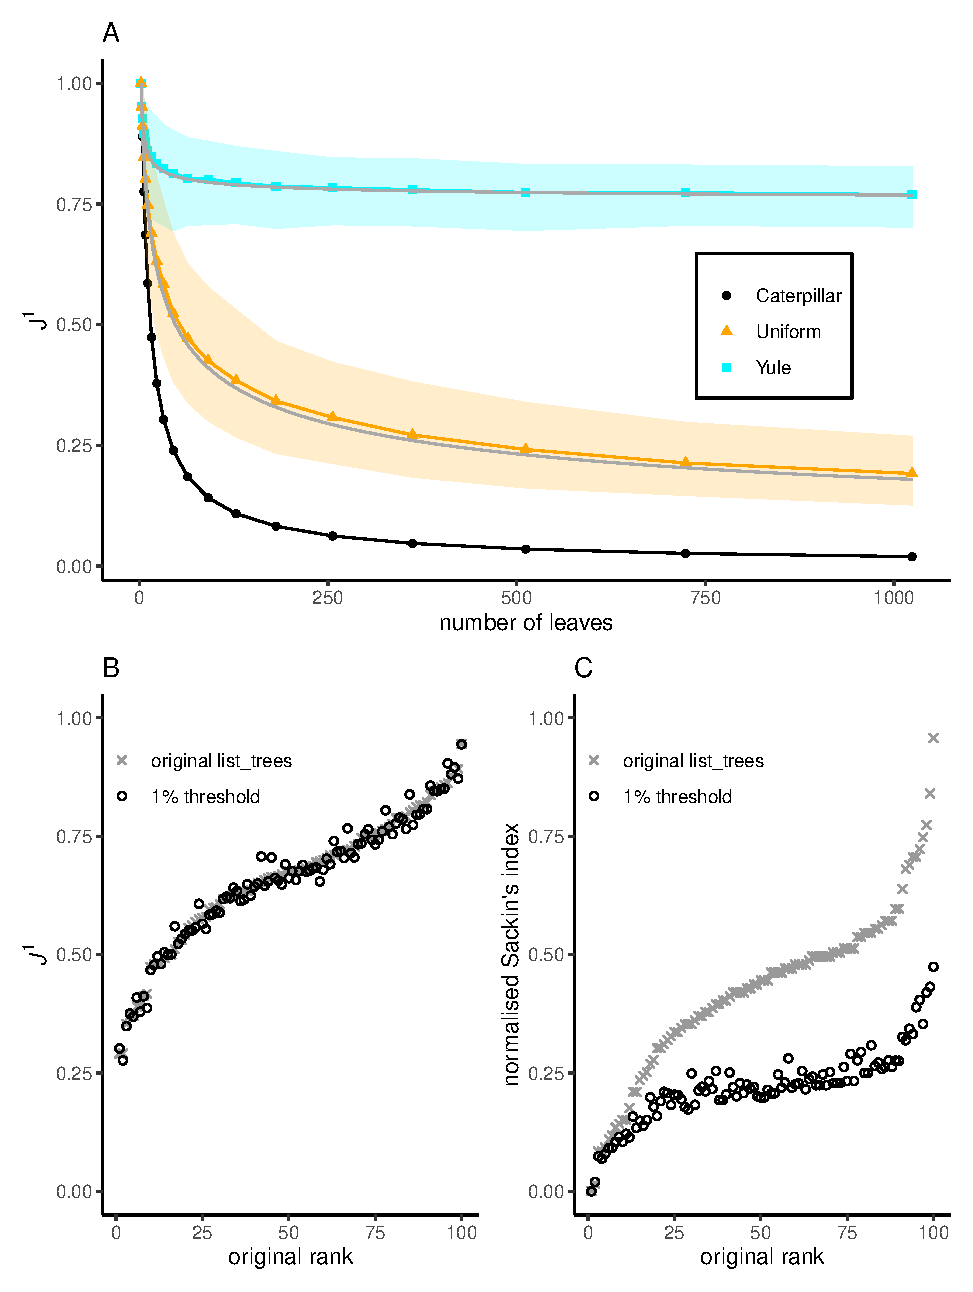
\includegraphics[width=0.82\textwidth]{Chapter_1/figures/old_j1_paper_figure.pdf}
    \caption{\textbf{A} $J^1$ values for trees generated under the Yule process and
    the uniform model. Solid grey curves represent the approximate expected values, and
    the dashed lines the $5$th and $95$th percentiles. \\
    \textbf{B} $J^1$ values for $100$ random
    trees on $16$ leaves using the alpha-gamma model, with $\alpha\sim \text{Unif}(0,1)$
    and $\gamma\sim \text{Unif}(0,\alpha)$. The values were
    calculated before and after applying a $1\%$ population threshold, i.e. removing all leaves
    with sizes smaller than $0.01$ times the total population.\\
    \textbf{C} Normalised Sackin index values for the same trees as in \textbf{B}.}
    \label{fig:robustness}
\end{figure}
\clearpage


\section{Agent-based modelling in oncology}

\subsection{Introduction}
Agent-based models (ABMs) are a class of computational models that simulate the actions and interactions of individual
agents within a system. These agents can represent anything from cells in a tissue to animals in an ecosystem. ABMs
are particularly useful in cancer research, as they can capture the complex interactions happening on the microscale in
cancer. Spatial agent-based models (SABMs) are a subclass of ABMs that incorporate spatial information into the
simulations. This is particularly useful for modelling solid tumours as it allows for the simulation of things like
the spatial heterogeneity of the tumour microenvironment and the effects of spatial constraints on tumour growth.
A strength of ABMs is that they can be as simple or as complex as the researcher needs them to be \cite{colyer_seven-step_2023}.
However, therein lies their weakness, as oversimplification of a model can lead to rapid loss of its utility in
capturing the behaviour of a complex system such as cancer. On the other hand, a model that is too complex, and
attempts to include everything from epigenetic mutations to the effects of the immune system on the tumour, is likely
too computationally expensive to be useful for modelling a tumour of reasonable size. This is an organic demonstration
of many a researcher's favourite saying \textit{all models are wrong, but some are useful, and some are more useful
than others}. In parsing through the literature and developing a new model of our own, we have also been influenced
by an alternative wording of this, that is \textit{the best model is its own worst enemy}, by Philip Maini. Our
interpretation is that a good model should address the questions it was designed to answer, but also open up new
ones which require further investigation, improvements, and research. For example, one can use our demon-warlock
framework \cite{bak_warlock_2023} to simulate the evolution of a tumour in space and draw conclusions on how
spatial organisation will impact intratumour heterogeneity or patient outcomes \cite{noble_when_2020, noble_spatial_2022}.
However, the model does not address the impact of the immune system, spatial heterogeneity in the microenvironment,
or the effects of therapy without further modifications. Alternatively, we may want to include diffusion of
nutrients and waste products in the model, or the effects of hypoxia on the tumour cells. Tools that would be
appropriate for such tasks are, for example, HAL \cite{bravo_hybrid_2020} or PhysiCell \cite{ghaffarizadeh_physicell_2018},
but they are not ideal either as simulating a realistically-sized tumour with these models is prohibitively expensive
in terms of computational resources. Thus, our preferred approach is to develop a proprietary model which is
informed by the literature and the data, and which has ample room for future expansion and improvement.

\subsection{The \texttt{demon-warlock} framework}
In a recent paper \cite{bak_warlock_2023}, we formally introduced a new agent-based model for simulating the
evolution of a tumour in space. The model is designed to be versatile and able to simulate a wide range of
spatial configurations and evolutionary properties of cancer. Spatially, the model is based on a 2D grid, where
each grid cell represents a deme, that is a spatially homogeneous population of cells. Each cell in the model
belongs to a genotype, a unique identifier based on the cell's mutations, and a driver genotype, which differentiates
itself from the genotype by not taking into account passenger mutations. Cell migrations in the tumour have multiple
modes, including invasion of tissue and other demes, and deme fission. The latter allows for the simulation of
tumours with a glandular structure, such as colorectal cancer. Events in the model are scheduled according to the
Gillespie algorithm, with the event hierarchy shown in figure \ref{fig:demon_events}. As the model was written
predominantly in plain C, it is highly efficient considering the complexity of the simulations it can run. An
accompanying R package, \texttt{demonanalysis}, is available for the analysis and visualisation of the model's
output, e.g. figure \ref{fig:demonanalysis_example}. \par
Despite the model's versatility, it is not without its limitations. In its current form, it is not feasible to
simulate tumours larger than a few million cells. This leaves out the possibility of simulating realistically-sized
glandular tumours which can contain a few million glands containing thousands of cells each at the time of diagnosis.
Furtermore, as the main limitation of the model's scalability is tied to the inherent inefficiency of generating
random numbers, it is not well-suited to simulating neutral stochastic markers, such as fluctuating methylation
clocks \cite{gabbutt_fluctuating_2022}. This is further discussed in section \ref{section:old_famework}.

\begin{figure}[h]
    \centering
    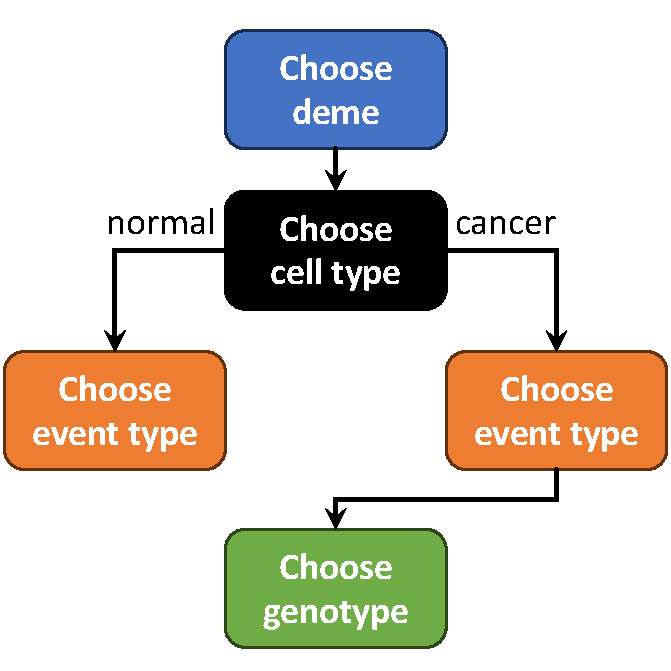
\includegraphics[width=0.75\textwidth]{Chapter_1/figures/demon_hierarchy.pdf}
    \caption{Event hierarchy in the \texttt{demon-warlock} framework. Figure reproduced from \cite{bak_warlock_2023} with
    the authors' permission.}
    \label{fig:demon_events}
\end{figure}

\begin{figure}[h]
    \centering
    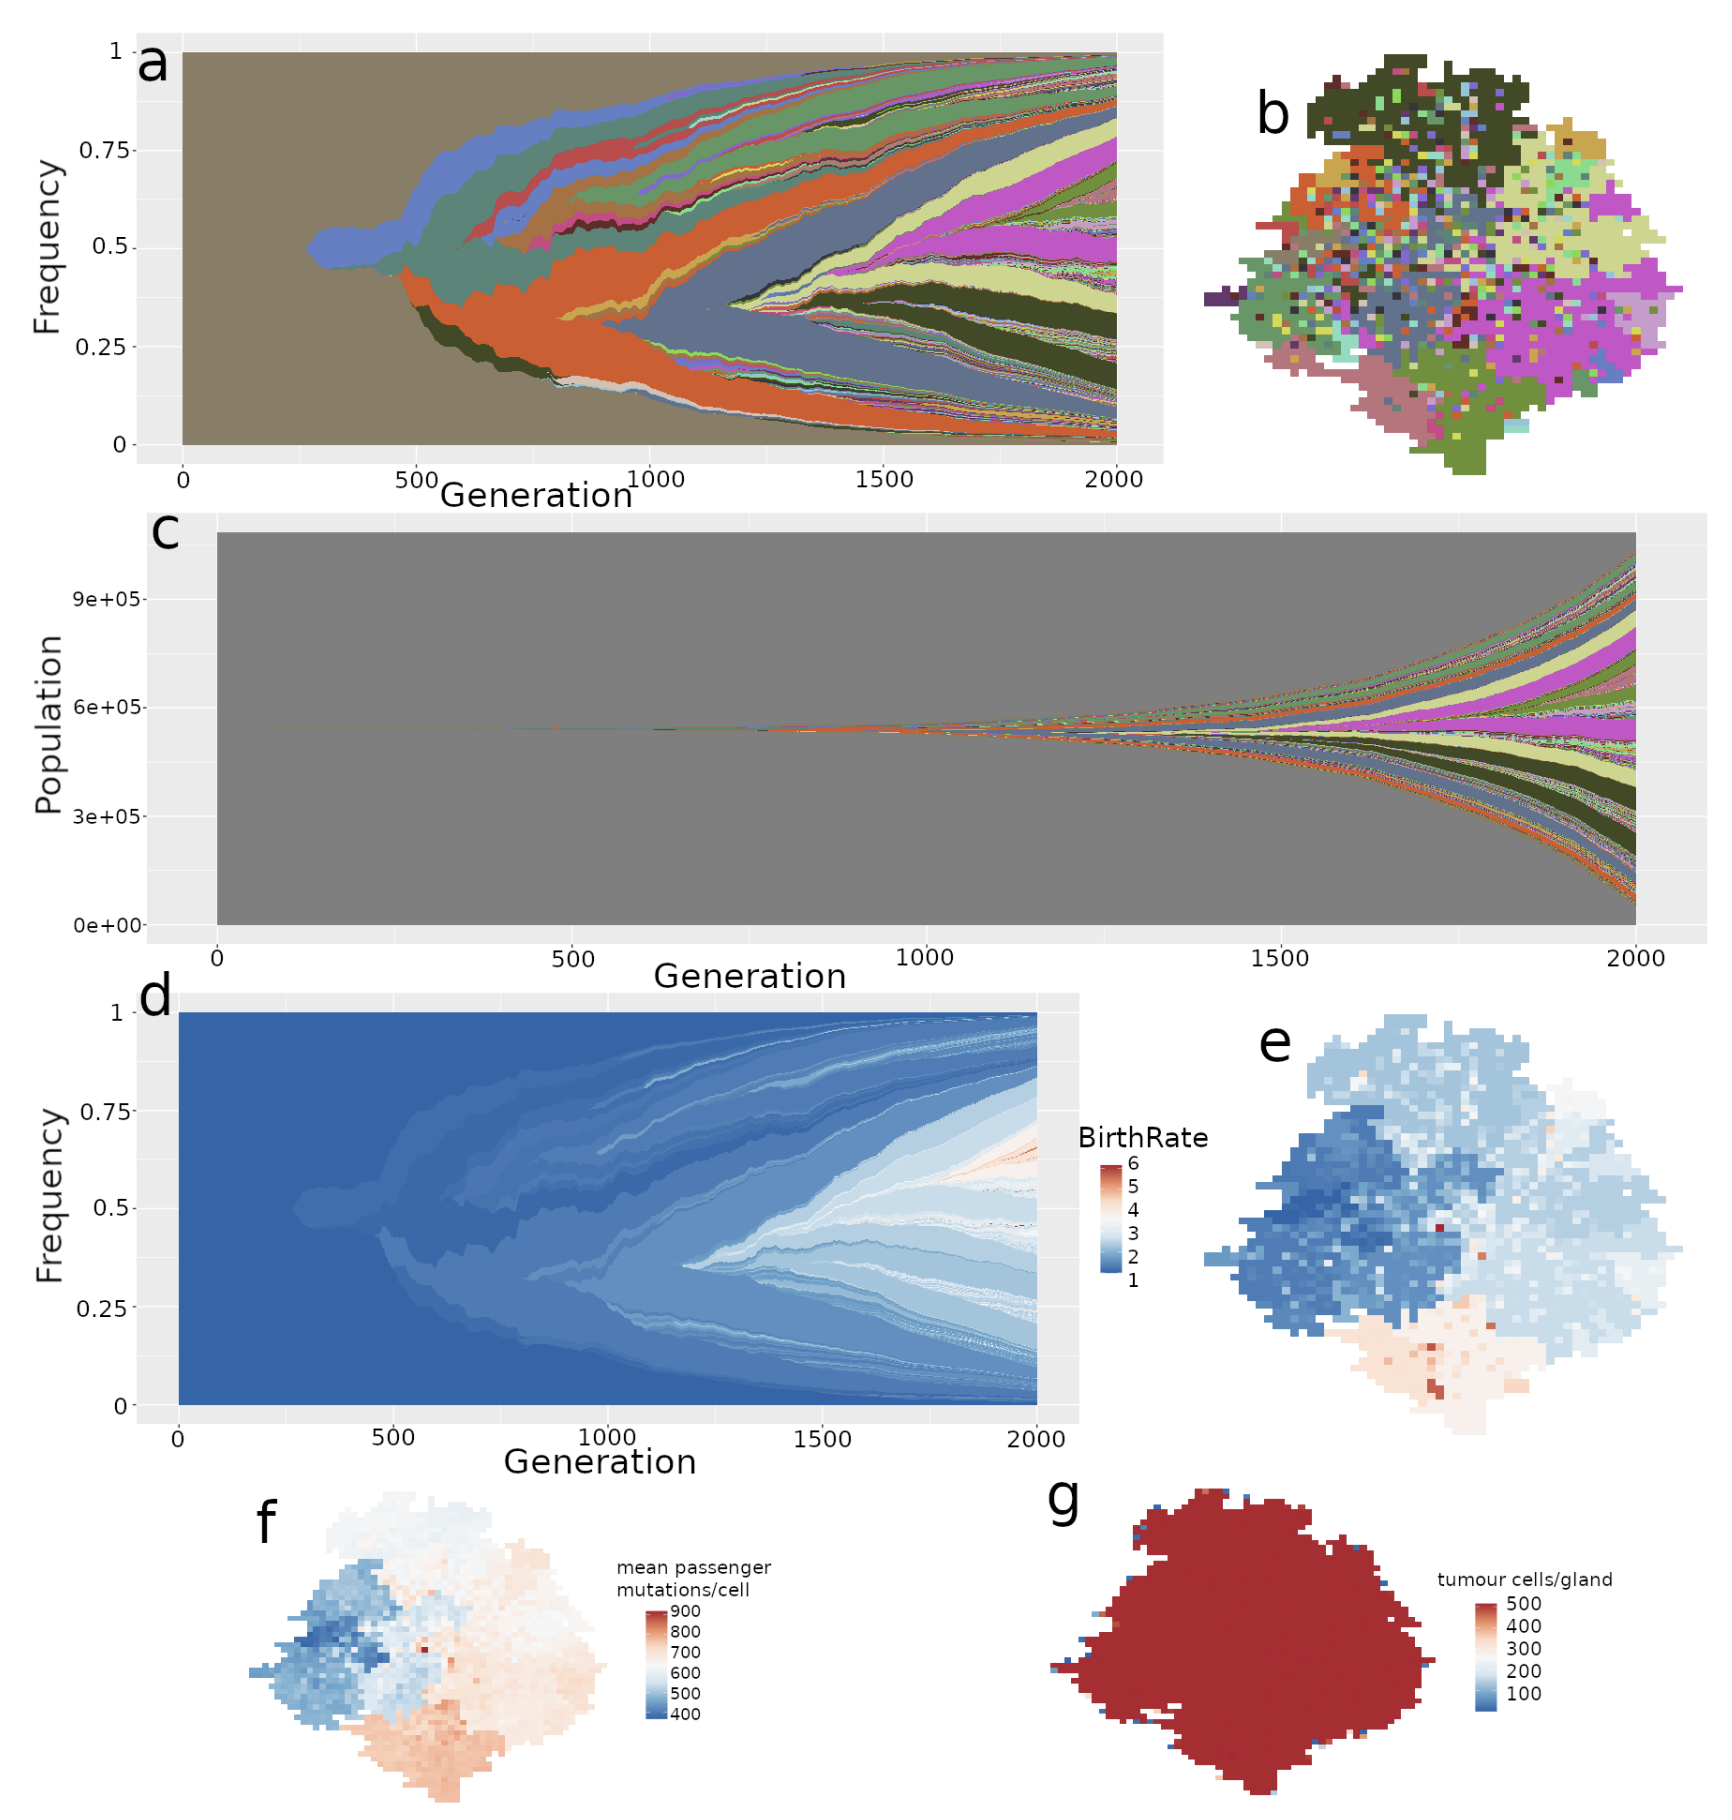
\includegraphics[width=\textwidth]{Chapter_1/figures/demonanalysis_example.png}
    \caption{Example output from \texttt{demon}, visualised using the \texttt{demonanalysis} package.
    \textbf{a} Muller plot of clonal dynamics over time. Each colour represents a clone with a distinct
    combination of driver mutations.
    \textbf{b} Final proportions and spatial plot of clones.
    \textbf{c} Fish plot of clone populations over time using the same colours as in \textbf{a}.
    \textbf{d} Muller plot showing evolution of tumour cell division rate.
    \textbf{e} Final spatial distribution of cell division rates.
    \textbf{f} Final spatial distribution of the mean numbers of passender mutations per cell.
    \textbf{g} Final spatial distribution of the number of tumour cells per gland.}
    \label{fig:demonanalysis_example}
\end{figure}
\clearpage

\section{Likelihood-free inference}
\subsection{Introduction}
To verify whether a model predicts behaviour of the observed system, a common approach is comparing its
output to measurements. The way this is done depends on the complexity of the model and the data. Here
we discuss the general framework of likelihoo-free inference, and more specifically the use of Approximate
Bayesian Computation (ABC). \par
Models based on differential equations can be compared to data using likelihood-based methods. In the
frequentist tradition, the likelihood function is used to estimate the parameters of the model under the
assumption that there is a correct, or ``true" value of those parameters. An alternative approach is
Bayesian statistics, which uses random variables ($\theta$) to represent the uncertainty in the parameters. The
distribution of these random variables before observing the data is called the prior distribution ($P(\theta)$).
After performing measurements in the system and obtaining data ($D$) which has an associated likelihood function
($P(D|\theta)$), the prior distribution is update to the posterior distribution ($P(\theta|D$)) using Bayes' theorem
\cite{bayes_essay_1763}:
\begin{equation}
    P(\theta|D) = \frac{P(D|\theta)P(\theta)}{P(D)}
\end{equation}
The likelihood function is thus a key component of Bayesian statistics, quantifying the probability of observing
the data given the parameters of the model. However, its greatest asset is also its greatest weakness. Depending
on the complexity of the model and the data, the likelihood function can be difficult or impossible to calculate
analytically, or can be too computationally expensive to calculate numerically. This is especially true for
stochastic models, such as agent-based models, where the likelihood function is often intractable. \par
In the case of intractable likelihoods, a common approach is to use likelihood-free inference methods, designed
to approximate the posterior distribution without the need to calculate the likelihood function. These methods
rely on the generation of simulated data from the model, and the comparison of these simulations to the observed
data. Instead of calculating the likelihood fucntion, these methods often involve a process of simulation and
rejection. A common drawback of likelihood-free inference methods is that they can be computationally expensive,
as they often require a large number of simulations to obtain a good approximation of the posterior distribution.
However, as the computational power of modern computers increases, these methods are becoming more and more
feasible for a wide range of models and data.

\subsection{Approximate Bayesian Computation}
Approximate Bayesian Computation (ABC) is a likelihood-free inference method that has gained popularity in the
last three decades \cite{tavare_inferring_1997, lechevallier_integrating_2010, jagiella_parallelization_2017}.
The basic idea behind ABC is to approximate the posterior distribution of the parameters of a model by comparing
simulated data to observed data. \par
In the most general form of ABC, the algorithm proceeds as follows:
\begin{enumerate}
    \item Sample a set of parameters from the prior distribution, $\hat\theta$.
    \item Simulate data from the model using the parameters.
    \item Compare the simulated data ($\hat D$) to the observed data ($D$) using a distance function, $d(\hat D, D)$.
    \item If the distance between the simulated and observed data is less than a certain threshold $\epsilon$, accept the
    parameters. Otherwise, reject them.
    \item Repeat steps 1-4 until a sufficient number of accepted parameters have been obtained.
\end{enumerate}
The distance threshold must be strictly positive, and is often chosen to be a small value. The choice of the distance
function is crucial, as it determines how the simulated data is compared to the observed data. Alternatively, in the
case of high-dimensional data, the distance function can be replaced by a summary statistic, $S$, which is a function of the
data, i.e. $d'(S(\hat D), S(D))$. The choice of summary statistics is also crucial, as it determines how the data is
reduced before the comparison. \par
ABC does not come without its own set of challenges. As it relies on comparing relevant features of the simulated data to
the observed data, the choice of summary statistic or distance metric is crucial, as it determines how the data is
reduced before the comparison. Fortunately, there are methods for reducing dimensionality of the data which
narrows in on its informative aspects \cite{blum_comparative_2013}.
The choice of the distance threshold is also essential, as it determines
the acceptance rate of the algorithm. Setting the threshold too high or too low can lead to biased or inefficient
estimates of the posterior distribution. However, this can be mitigated by using a dynamic threshold, which is
adapted during the course of the algorithm \cite{prangle_adapting_2017}.
Finally, the computational aspects of ABC must be mentioned, as the algorithm relies on repeated simulations of
potentially complex models. This can require a large amount of computational resources, raising questions about
the method's scalability and practicality. An obvious way to circumvent this is to use a model which is as
lightweight as possible. Even in the case of infinite compute available, one must be mindful of the fact that
the more complex the model, the more complex the inference problem, and the more complex the inference problem,
the more complex the model. This is a feedback loop which can render both the model and subsequent analysis
uninterpretable. Therefore, we believe that the best practice as a mathematician and applied scientist is to abstract
the model enough to be able to draw conclusions from it, but not so much that it becomes uninformative. \par
In chapter \ref{chapter:methdemon}, we introduce our simplified model of colorectal cancer gland fission and
the accompanying ABC workflow. We discuss the choice of summary statistics and the performance of the ABC
algorithm, and subsequently demonstrate the model's utility in inferring the evolutionary history of a tumour
from methylation data in chapter \ref{chapter:methylation}.


\section{Fluctuating methylation clocks}
The concept of a molecular clock is a hallmark of evolutionary biology. It is based on the idea that the
rate of evolution of a particular gene or set of genes is constant over time, and can be used to estimate
the time of divergence between species or the time of a particular event in the evolutionary history of a
species. The most famous example of a molecular clock is the mitochondrial DNA clock, which is used to
estimate the time of divergence between species \cite{hasegawa_dating_1985}. The key principle behind molecular
clocks is that closely related species or individual will have more similar sequences than distantly related
ones. This also translates to individual cells in cancer. The issue with using molecular clocks in cancer
is that ``slowly ticking" molecular clocks, i.e. ones with a low mutation rate, are not informative enough
on the timescale of cancer evolution, limiting their utility to cell lineages which diverged too far in the past,
with recent events remaining undetectable. On the other hand, ``fast ticking" molecular clocks can
reveal recent evolutionary events but also have their own limitations, such as independent mutations in the
same site \cite{kuipers_single-cell_2017}. \par
\textit{TO DO:} Introduce and discuss FMCs.



\section{Aims and objectives}

\subsection{Hypotheses}
\begin{enumerate}
    \item The $J^1$ index is a universal measure of tree balance, and can be used, in conjunction with other
        tree shape indices, to differentiate between evolutionary modes in cancer.
    \item Spatial agent-based models are a powerful tool for simulating the evolutionary dynamics of solid tumours.
    \item These methods are useful for inferring the evolutionary history of colorectal cancer based on multi-site
        methylation array sequencing.
\end{enumerate}

\subsection{Aims}
\begin{enumerate}
    \item Calculate or approximate important properties of the $J^1$ index, such as its expected value under
        standard tree-generating processes.
    \item Determine the utility of sets of tree shape indices for differentiating between evolutionary modes in cancer.
    \item Extend the fluctuating methylation clock model to multi-site sequencing of solid tumours on the
        example of colorectal cancer.
\end{enumerate}

\subsection{Objectives}
\begin{enumerate}
    \item Contextualise $J^1$ within the broader field of tree shape indices in biology and computer science.
    \item Investigate extreme and expected values of $J^1$ under standard tree-generating processes.
    \item Recapitulate the classification of evolutionary modes in cancer using a set of three tree shape indices.
    \item Extend the discussion to a more interpretable and general system of tree shape indices.
    \item Develop an agent-based model for simulating the evolutionary dynamics of colorectal adenocarcinoma.
    \item Develop an ABC workflow for inferring the evolutionary parameters of the model, specifically the
        gland fission rate, methylation and demethylation rates, driver mutation rate, selective advantage,
        and the effective number of lineages per tumour gland.
    \item Apply the model to colorectal cancer data and compare the inferred phylogenies to the trees generated
        by the model.
\end{enumerate}


\chapter{Expected and extreme values of universal tree balance index $J^1$}\label{chapter:trees}


\section{Introduction}
Broadly speaking, the balance of a tree is the extent to which its terminal nodes (leaves)
are evenly distributed among its branches. Despite the abundance of metrics of tree balance
\cite{fischer_tree_2021}, universal indices are hard to come by. This limits practical
applications of tree balance indices. \par
Following the $J^1$ index paper \cite{lemant_robust_2022}, where a universal index was proposed,
shown to be robust to the removal of small nodes and to outperform conventional tree balance
indices as a summary statistic for comparing model output to empirical data, I examined several
important properties of $J^1$. Given any new tree shape index, the expected value under standard
tree-generating processes and the extreme values need to be known for the index to be useful in
practice. In figure \ref{fig:robustness}A, I showed the sample mean of $J^1$ up to 128 leaves
under the Yule and uniform models, which appears to be close to the inverse Sackin index
expression derived by Noble in \cite{lemant_robust_2022}. Additionally, as a consequence of this
relationship, the caterpillar trees minimises $J^1$ for bifurcating trees. However, I showed in
\cite{lemant_robust_2022} that the caterpillar topology does not minimise $J^1$ for multifurcating
trees by providing a couterexample on $6$ leaves. \par
In this chapter, I will further show the universality of $J^1$ by identifying fundamental
connections to classical results in computer science, related to Huffman coding and self-balancing
tree data structures. I will also derive upper bounds on the error of the expected value
approximations for the Yule process and uniform model. For the Yule process, I show that the
approximation rapidly converges to the true expected value in the large tree limit. Finally,
I will investigate the minimal values of $J^1$ in important special cases, obtaining a
counter-intuitive result in the large tree limit.


\section{Prerequisites}


\subsection{Preliminary definitions from systematic biology}\label{defsec}

\begin{definition}[Rooted tree]
    A \textbf{rooted tree} $T$ is a connected acyclic graph with node set $V(T)$
    and edge (or branch) set $E(T)$, in which one node is designated the root.
    Parent-child and ancestor-descendant relationships in a rooted tree are
    assigned along paths directed away from the root.
\end{definition}

\begin{definition}[Node size and tree magnitude, \citet{lemant_robust_2022}]
    We assign to every node a non-negative size. The \textbf{magnitude} of a
    tree $T$, denoted $S(T)$, is then the sum of its node sizes.
\end{definition}

\begin{definition}(Leafy tree, \citet{lemant_robust_2022})
    A \textbf{leafy tree} is one with only zero-sized internal nodes.
\end{definition}

\begin{definition}(Node depth)
    As we will consider only trees with uniform edge lengths, we define the
    \textbf{depth} of a node as the number of edges in the shortest path from
    that node to the root.
\end{definition}

\begin{definition}[Sackin index, \citet{sackin_good_1972}]
    The \textbf{Sackin index} of rooted tree $T$ is the sum of its leaf depths:
    \begin{equation}\label{sackindef}
        I_S(T) = \sum_{l\in L(T)} \nu(l),
    \end{equation}
    where $L(T)$ is the set of all leaves (terminal nodes) of $T$, and $\nu(l)$
    is the depth of leaf $l$.
\end{definition}

\begin{definition}[Generalised Sackin index, \citet{lemant_robust_2022}]
    The Sackin index can be generalised to account for arbitrary node sizes:
    \begin{equation}\label{gensackindef}
        I_{S,\text{gen}}(T) = \sum_{i\in V(T)} S_i^*,
    \end{equation}
    where $V(T)$ is the set of all internal nodes (non-leaves), and $S_i^*$ is
    the magnitude of the subtree rooted at node $i$, excluding $i$. If $T$ is a
    leafy tree in which all leaves have unit size then
    $I_{S,\text{gen}}(T) = I_S(T)$.
\end{definition}

\begin{definition}[Robust balance index, \citet{lemant_robust_2022}]\label{j1defn}
    The robust balance index $J^1$ of tree $T$ is
    \begin{equation}\label{J1def}
        J^1(T) = \frac{1}{I_{S,\text{gen}}(T)} \sum_{i\in\tilde{V}(T)} S_i^{*}
        \sum_{j\in C(i)}W_{ij}^{1},
    \end{equation}
    where $\tilde{V}(T)$ the set of all internal nodes whose descendants are not
    all of zero size, $C(i)$ is the set of children of node $i$, and $W_{ij}^1$
    is the node balance score, defined as the normalised Shannon entropy of the
    daughter subtree magnitudes:
    \begin{equation}\label{Wij1}
        W_{ij}^1 =
        \begin{cases}
            -\frac{S_j}{S_i^*}\log_{d^+(i)}\frac{S_j}{S_i^*},& \text{ for } d^+(i) > 1\\
            0, & \text{ otherwise,}
        \end{cases}
    \end{equation}
    where $S_i$ is the magnitude of the subtree rooted at node $i$, including
    $i$, and $d^+(i)$ is the outdegree of $i$.
\end{definition}

\begin{definition}[Binary tree and bifurcating tree]
    A \textbf{binary tree} is a rooted tree in which no node has more than 2
    children. A \textbf{bifurcating tree} (or full binary tree) is a rooted tree
    in which each internal node has exactly 2 children.
\end{definition}

\begin{definition}[Cherry]
    A tree consisting of only a root and two leaves is a \textbf{cherry}.
\end{definition}

\begin{definition}[Caterpillar tree]
    A \textbf{caterpillar tree} is a bifurcating tree in which every internal
    node except one has exactly one child leaf.
\end{definition}

\begin{definition}[Fully symmetric tree]
    If, for every internal node $i$, the subtrees rooted at the children of $i$
    all contain the same number of leaves then the tree is \textbf{fully symmetric}.
\end{definition}

\subsection{Preliminary definitions from computer science}\label{compscisec}

\begin{definition}[Root balance and tree balance scores, \citet{nievergelt_bounds_1972}]
    The \textbf{root balance score} of a bifurcating leafy subtree $T_i$ rooted
    at $i$ and containing at least three nodes is
    \begin{equation}
        \rho(T_i) = \frac{\min(S_{i_1}, S_{i_2})}{S_i} \in \left[0, \tfrac{1}{2}\right],
    \end{equation}
    where $S_i$ is the magnitude of $T_i$, and $S_{i_1}$ and $S_{i_1}$ are the
    magnitudes of the subtrees rooted at the children of $i$. The balance score
    of a bifurcating leafy tree $T$ is then defined as
    \begin{equation}\label{defballeafy}
        \beta(T) = \min\left( \rho(T_i)_{i\in V(T)} \right).
    \end{equation}
    For any given leaf count, the balance score is minimal for the caterpillar
    tree and maximal for the fully symmetric bifurcating tree.
\end{definition}

\begin{definition}[Total and weighted path lengths, \citet{nievergelt_bounds_1972}]
    In computer science, the Sackin index is better known as the \textbf{total path length}.
    Let $T$ be a rooted tree in which each node $i$ is assigned a weight
    (or access frequency) $w_i$. Then the \textbf{weighted path length} of $T$ is
    \begin{equation}\label{wpathdef}
        |T| = \sum_{i \in V(T)} w_i \nu(i).
    \end{equation}
\end{definition}


\section{Results}


\subsection{$J^1$ unites and generalises prior notions of tree balance}

In computer science, tree balance is effectively a binary property: a tree is
considered balanced if its weighted path length is sufficiently small, given its
leaf count \citep{nievergelt_binary_1972}. In biology, where comparisons between
trees are more relevant, researchers instead use a normalised form of the Sackin
index or various other indices to assign balance values on a continuum
\citep{colless_review_1982, shao_tree_1990, mir_new_2013, mir_sound_2018, fischer_tree_2021}.
I will show that $J^1$ uniquely connects these two historically separate
notions of tree balance.
Let us note first that the weighted path length is equivalent to the generalised Sackin index:

\begin{equation}
    |T| = \sum_{i \in V(T)} \alpha_i \nu(i) = \sum_{i\in V(T)} S^*_i = I_{S, gen}(T).
\end{equation}

Consider then the following proposition.

\begin{proposition}[\citet{lemant_robust_2022}] \label{proposition6}
    Let $T$ be a leafy tree with $d^+(i) = m > 1$ for all internal nodes $i$. Then
    \begin{equation}
        J^1(T) = \frac{H_m(T)S(T)}{I_{S,\text{gen}}(T)}, \label{prop6}
    \end{equation}
    where $H_m(T)$ is the Shannon entropy (base $m$) of the proportional leaf sizes.
\end{proposition}

\begin{corollary}
    We can rewrite equation \eqref{prop6} for bifurcating trees as
    \begin{equation}
        J^1(T) = \frac{H_2(T)S(T)}{|T|}. \label{corr6}
    \end{equation}
    Hence, for any given set of leaf sizes, minimising the weighted path length
    is equivalent to maximising $J^1$.
\end{corollary}

\begin{theorem}[Section 5 of \citet{nievergelt_bounds_1972}]\label{thm2}
    Let $T$ be a bifurcating leafy tree with balance score $\beta_T$. Then the
    total path length $|T|$ satisfies the inequality
    \begin{equation}
        |T| \leq \frac{S(T)\log_2S(T) + H_2(T)}{H_2(\beta_T)}.
    \end{equation}
    If the node sizes sum to unity then this simplifies to
    \begin{equation} \label{thm2eqn}
        |T| \leq \frac{H_2(T)}{H_2(\beta_T)}.
    \end{equation}
\end{theorem}

A special case of this theorem is considered as Theorem 2 in \citet{wong_upper_1973}:
If the tree has $n$ leaves, all of size 1 then
    \begin{equation}\label{thm2eqnspecial}
        |T| \leq \frac{n\log n}{H(\beta_T)}.
    \end{equation}
The proof of this theorem defines the \textit{average entropy} of a general tree
$T$, corrected for typo in original paper, as
\begin{equation}
    \bar{H}(T) = \frac{1}{|T|}\sum_{k\in\tilde{V}(T)}\sum_{j\in C(k)}n_j\log_2\frac{n_k}{n_j},
\end{equation}
which is identical to the definition of $J^1$, equation \eqref{J1def}, up to the
base of the logarithm in the expression for the entropy of internal node $k$.

\begin{remark}
    We can trivially expand the definition of the balance score to $m$-furcating
    trees, by considering all $m$ descendants of internal nodes in the root
    balance score. The root balance score of subtree $T_j$ rooted in node $j$
    of $m$-furcating leafy tree $T$ can be defined as
    \begin{equation}
        \rho_m(T_j) = \frac{\text{min}(S_{j_1}, \dots, S_{j_m})}{S_j},
    \end{equation}
    where $j_1,\dots,j_m\in C(i)$ are the children of node $j$. By extension, we define
    \begin{equation}
        \beta_m(T) = \text{min}(\rho_m(T_i)_{i\in V(T)}),
    \end{equation}
    the balance score of $m$-furcating leafy tree $T$.
\end{remark}

\begin{corollary}\label{j1_lower_bound_cor}
    There is a lower bound on $J^1$ for an $m$-furcating leafy tree $T$ on $n$
    leaves, with balance score $\beta_T$, and it equals
    \begin{equation}\label{j1_lower_bound}
        J^1_\text{lower} = \frac{H_m(T)S(T)}{|T|_\text{upper}} = \frac{n\log_mn}
        {(H_m(\vec\beta_T))^{-1}n\log_mn} = H_m(\vec\beta_T).
    \end{equation}
    where $\vec\beta_T = (S_{1,min}, \dots, S_{m, min})$ is the vector of
    magnitudes of subtrees rooted in the children of the node with the smallest
    root balance score.
\end{corollary}

The connections between $J^1$ and measures of tree balance and entropy in
computer science show that these properties are universally important.
However, the similarities may well end at this point, as evolutionary
biologists and computer scientists use these measures for different purposes
and take their research in opposite directions directions, for example inferring
evolutionary processes which produced the tree shape \citep{mooers_inferring_1997}
versus shaping the tree to optimise data storage and retrieval \citep{nagaraj_optimal_1997}.

\subsection{$J^1$ is maximised by Huffman coding}

\begin{definition}[Binary search tree]
    A \textbf{binary search tree} $T_n$ over $n$ entries (w.l.g. numbers)
    $x_1,\dots,x_n$ is a labelled binary tree, each of whose nodes have been
    labelled with a distinct number chosen from $x_1,\dots,x_n$ such that for
    each node $N$, all nodes in the left subtree of $N$ have a smaller
    $x_i$ as their label than $x_N$, and all nodes in the right subtree of $N$
    have a larger number as their label than node $N$ (e.g. figure \ref{example_bst}).
\end{definition}

\begin{figure}[h]
    \centering
    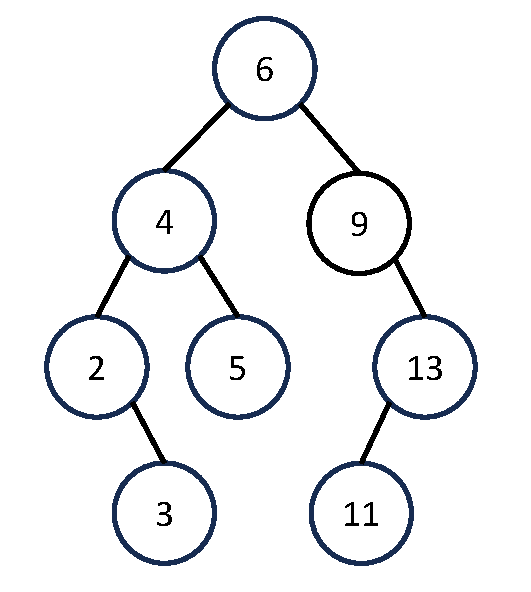
\includegraphics[width=.5\textwidth]{Chapter_2/figures/example_bst.pdf}
    \caption{A simple example of a binary search tree over the set of labels $S
    = \{2,3,4,5,6,9,11,13\}.$}
    \label{example_bst}
\end{figure}

\begin{remark}
    Each node $i$ in a binary search tree can have an associated non-negative
    number called access frequency (or weight, size, probability) $w_i$.
\end{remark}

To construct an optimal binary search tree, that is one with a minimal weighted
path length, we can use Huffman coding.

\begin{definition}[Huffman coding, \citet{huffman_method_1952}]
    Let $A = (\alpha_1, \dots, \alpha_n)$ be a tuple of non-negative numbers.
    To construct an optimal binary tree on $n$ leaves with sizes given by $A$
    we choose the two smallest ones, w.l.g. $\alpha_1$ and $\alpha_2$, and
    join them in a cherry, so that their parent node has size $\alpha_1 + \alpha_2$.
    We now have $A' = (\alpha_1 + \alpha_2, \alpha_3, \dots, \alpha_n)$ as our
    set of $n-1$ nodes. By repeating this procedure until we have only one node
    left, an optimal binary search tree is obtained.
\end{definition}

\begin{proposition}
    The Huffman method maximises $J^1$ on bifurcating trees for a given set of node sizes.
\end{proposition}

\begin{proof}
    By corollary \ref{j1_lower_bound_cor}, the Huffman method maximises $J^1$
    as it minimises the weighted path length.
\end{proof}

As Huffman coding is an optimisation algorithm, $J^1$ can be used to measure how
close a tree constructed using a given set of node sizes is to the maximally
balanced binary tree on the same set. This means we can quantify how close an
alternative algorithm which runs in a faster time complexity, such as arithmetic
coding \citep{pasco_source_1977}, gets to the optimal solution.

\subsection{Expected value of $J^1$ under simple evolutionary processes}\label{expsection}

For applications in evolutionary biology, an important property of balance
indices is their expected value under an evolutionary process. This quantity
helps us compare the trees generated under a null model to the observed data,
and is a valuable part of inferring the underlying evolutionary properties.
Two of the simplest, and most widely studied, processes of tree generation are
the uniform model \citep{rosen_vicariant_1978} and the Yule model
\citep{yule_iimathematical_1925}, which generate bifurcating trees and are
useful null models in evolutionary biology. The Yule model, also known as the
pure birth or coalescent model, is used when considering speciation rates and
patterns \citep{aldous_stochastic_2001, steel_properties_2001}. The uniform
model is used as a null model for comparing neutral evolutionary patterns
against ones which include more complex biological mechanisms
\citep{mooers_inferring_1997, mckenzie_distributions_2000}. While in section
\ref{compscisec} I discussed the static calculation of a balance index for a
given tree, I am also interested in how balanced binary search trees generated
under some stochastic process are. The Yule model is also useful for these
considerations as it is connected to the BST martingale, a statistical tool
used to analyze and predict the behavior of binary search trees, via $L_1$
convergence \citep{chauvin_connecting_2004}. From here, one can extend the
discussion to AVL and red-black trees in a similar way to more complex
evolutionary processes as self-balancing trees will by definition have higher
expected values of $J^1$ than those generated under the Yule process. \par
The expected value of a few indices, and even some higher moments in certain
cases, are known for both Yule and uniform models
\citep{mir_new_2013, m_coronado_sackins_2020, goh_two_2022}. Among these is the
Sackin index, which is particularly useful for our purposes. \par

\begin{definition}[Yule model, \citet{yule_iimathematical_1925}]\label{yuledef}
    Consider a bifurcating tree $T$ on $n$ leaves. To obtain the probability of
    generating $T$ under the Yule model, start with a single node and replace it
    with a cherry. Then, at each step, choose one leaf uniformly at random and
    replace it with a cherry, until the tree has $n$ leaves (figure
    \ref{yule-unif-figure}A). The sum of probabilities of generating $T$ in all
    possible ways is the probability of generating $T$ under the Yule model.
\end{definition}

\begin{definition}[Uniform model, \citet{rosen_vicariant_1978}]\label{unifdef}
    Under the \textbf{uniform model} of tree generation, every bifurcating tree
    on $n$ leaves has an equal probability of being generated, which is equal to
    $n\binom{2n-2}{n-1}^{-1}$ (figure \ref{yule-unif-figure}B).
\end{definition}

\begin{remark}
    We only consider leafy trees with equal leaf sizes generated by the
    processes in definitions \ref{yuledef} and \ref{unifdef}.
\end{remark}

\begin{remark}
    We calculated the exact values of the expectation of $J^1$ under both the
    Yule and uniform models semi-manually by creating all possible $(n+1)$-leaf
    trees given a set of $n$-leaf trees, eliminating duplicates and assigning
    appropriate probabilities in the Yule case, and thus computing the exact
    value of the expectation. The process is inefficient for large trees, and
    we limited our search to $n\leq 11$, the exact and approximate expected
    values for which are found in table \ref{table_values}.
\end{remark}

\begin{figure}[h!]
    \centering
    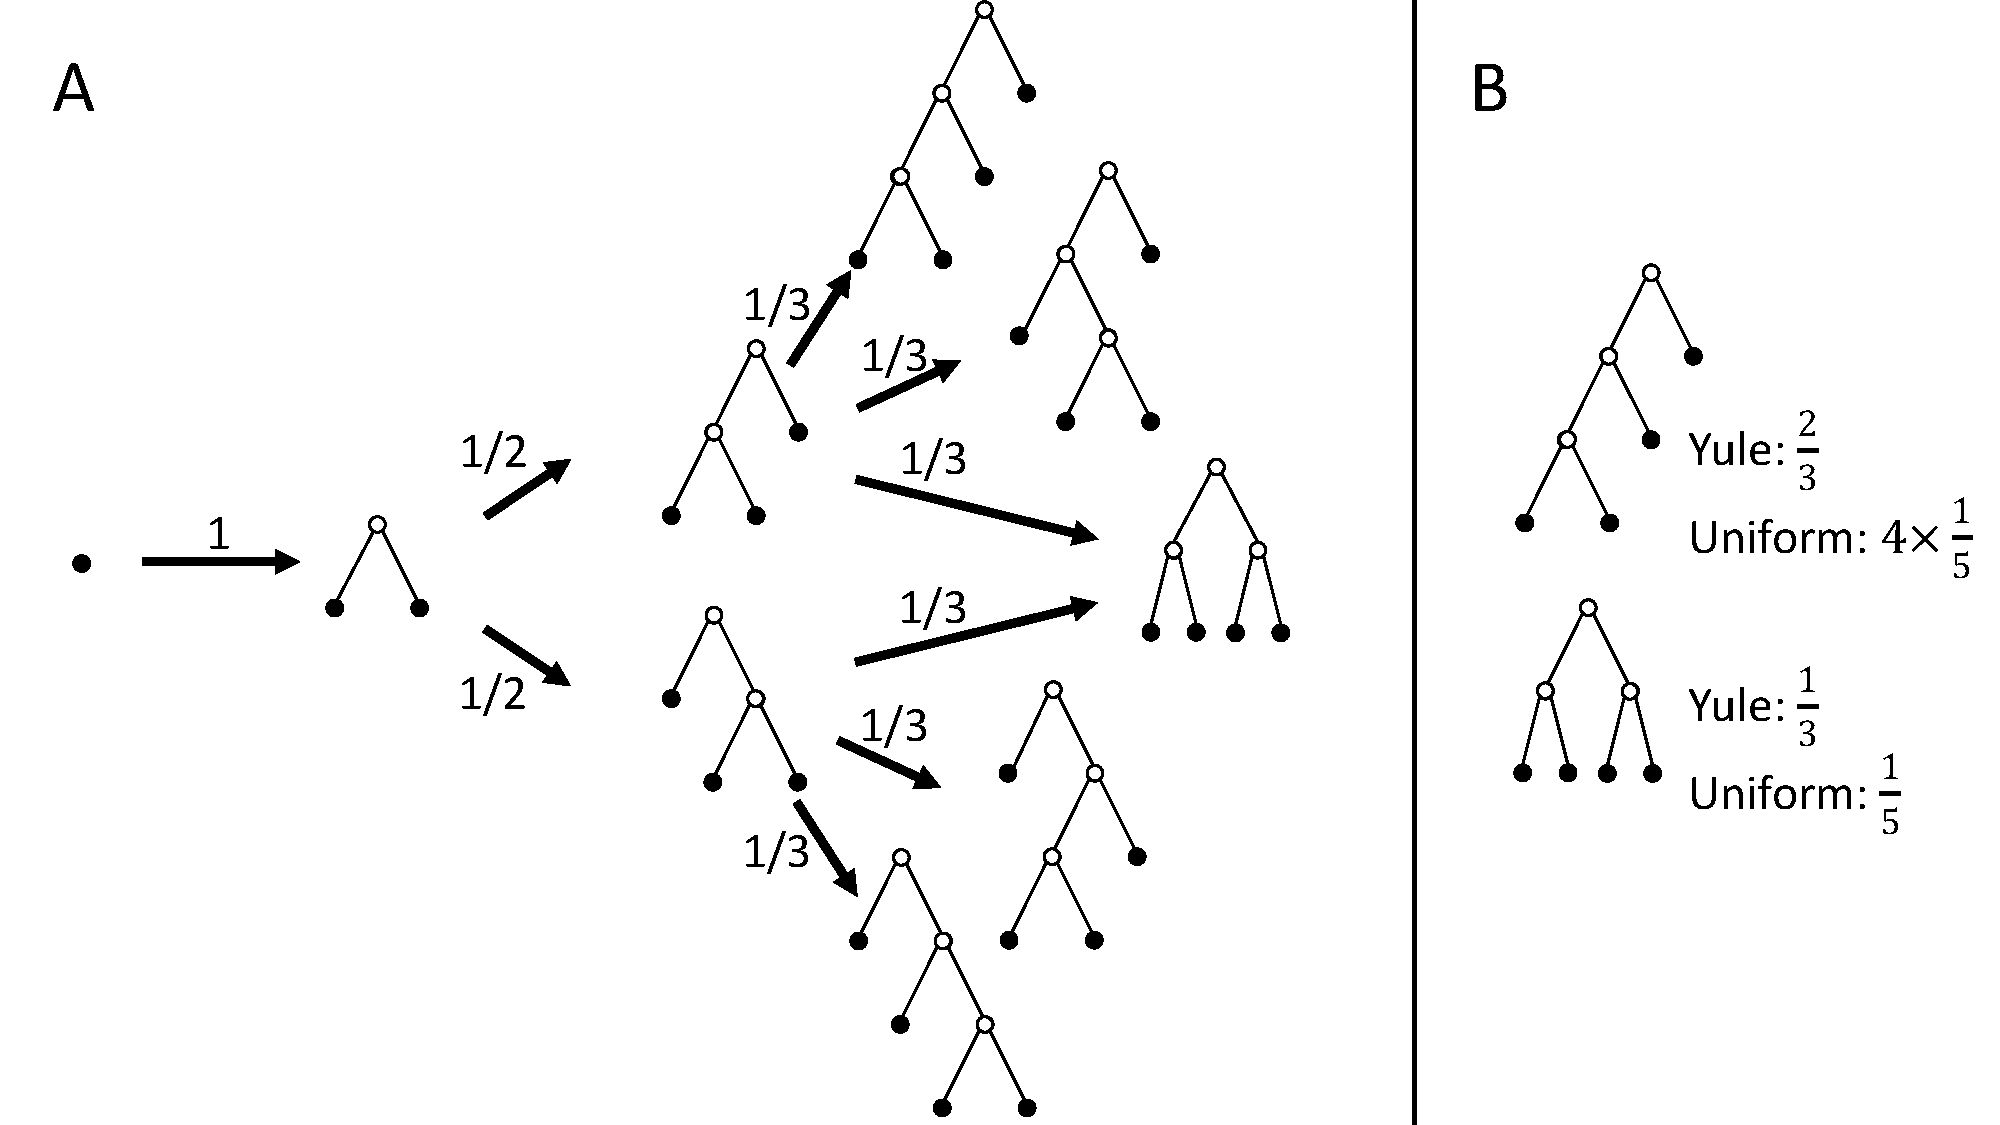
\includegraphics[width=\textwidth]{Chapter_2/figures/yule-unif-figure.pdf}
    \caption{Comparison of probabilities for generation of trees on $4$ leaves
    under the Yule and uniform models. \textbf{A:} Arrows show generation under
    the Yule model. Each of the trees shown on $4$ leaves has the same
    probability under the uniform model. \textbf{B:} Comparison of probabilities
    of tree topologies on $4$ leaves under the Yule and uniform models.}
    \label{yule-unif-figure}
\end{figure}

Under the Yule model, the expected value of the Sackin index for trees on $n$
leaves is
\begin{equation}
    \mathbb{E}_Y^n(I_S) = 2n\sum_{i=2}^n \frac{1}{i},
\end{equation}
as shown in \citet{kirkpatrick_searching_1993}. Equation \eqref{prop6} implies
then that the expected value of $J^1$ for a tree on $n$ leaves is
\begin{equation}
    \mathbb{E}_Y^n(J^1) = \mathbb{E}_Y^n(\frac{n\log_2 n}{I_S}) = n\log_2 n
    \mathbb{E}_Y^n(1/I_S),
\end{equation}
where $\mathbb{E}_Y^n(1/I_S)$ is the harmonic mean of the Sackin index.
The harmonic mean under the Yule process is not a standard result in literature,
nor have I been able to obtain a closed-form solution for this problem so far.
It is possible, however, to compare the harmonic and arithmetic means of $I_S$ by
considering the Jensen gap
\begin{equation}\label{JensenGap}
    \mathcal{J}(f, X) = \mathbb{E}[f(X)] - f(\mathbb{E}[X]),
\end{equation}
with $f(x) = 1/x$.

\begin{theorem}[\citet{liao_sharpening_2017}]\label{jensen_thm}
    Let $X$ be a one-dimensional random variable with mean $\mu$, and
    $P(X\in(a,b))=1$, where $\infty\leq a<b\leq \infty$. If $f(x)$ is a twice
    differentiable function on $(a,b)$, and
    \begin{equation}
        h(x;\nu) = \frac{f(x)-f(\nu)}{(x-\nu)^2} - \frac{f'(\nu)}{x-\nu},
    \end{equation}
    then
    \begin{equation}
        \inf_{x\in(a,b)}\{h(x;\mu)\}\mathrm{Var}(X) \leq \mathbb{E}[f(X)] -
        f(\mathbb{E}[X]) \leq \sup_{x\in(a,b)}\{ h(x;\mu) \}\mathrm{Var}(X).
    \end{equation}
\end{theorem}

\begin{proposition}\label{jensen_prop}
    Let $\mathbb{E}_Y(J^1)$ and $\mathbb{E}_U(J^1)$ be expectation values of
    $J^1$ under the Yule and uniform models respectively. Then:
    \begin{enumerate}[(i)]
        \item $\mathbb{E}_Y(J^1)\to\frac{n\log_2n}{\mathbb{E}_Y(I_S)}$,
        \item $\mathbb{E}_U(J^1)-\frac{n\log_2n}{\mathbb{E}_U(I_S)}$ is bounded
            from both sides,
    \end{enumerate}
    as $n\to\infty$.
\end{proposition}
\begin{proof}
    \textit{(i)} Let $\mu_Y$ be the expected value of the Sackin index under the
    Yule process for trees on $n$ leaves, and $f(x)=\frac{1}{x}$. By theorem
    \ref{jensen_thm}
    \begin{equation}\label{hxmuY}
        h(x;\mu_Y) = \frac{f(x)-f(\mu_Y)}{(x-\mu_Y)^2} - \frac{f'(\mu_Y)}
        {x-\mu_Y} = \frac{1}{x\mu_Y^2}.
    \end{equation}
    We can then substitute this into the inequality given in the theorem
    \begin{equation}\label{JensenApp}
        \frac{n\log_2n}{\frac{(n-1)(n+2)}{2}\mu_Y^2} \text{Var}_Y(I_S) \leq
        \mathbb{E}[J^1] - \frac{n\log_2n}{\mathbb{E}[I_S]} \leq \frac{n\log_2n}
        {\mu_Y^2n\log_2n}\text{Var}_Y(I_S),
    \end{equation}
    where the supremum and infimum of $h(x,\mu)$ are substituted with extremal
    values of the Sackin index on bifurcating trees
    \citep{fischer_extremal_2021}. The expectation of the Sackin index under the
    Yule process is given in equation \eqref{yule_exp_sackin}, and its variance
    is calculated as \citep{cardona_exact_2012}
    \begin{equation}\label{yulevarIS}
        \text{Var}_Y(I_S) = 7n^2 - 4n^2\sum_{i=1}^n\frac{1}{i^2} - 2n
        \sum_{i=1}^{n}\frac{1}{i} - n.
    \end{equation}
    Substituting these expressions into equation \eqref{JensenApp}, we find
    limits
    \begin{align*}
        \frac{n\log_2n}{\frac{(n-1)(n+2)}{2}\mu_Y^2} \text{Var}_Y(I_S) &
        \stackrel{n\to\infty}{\sim} \frac{\log n\left(7n^2 - 4n^2\sum_{i=2}^n
        \frac{1}{i^2}-2n\sum_{i=2}^n\frac{1}{i}-n\right)}{4n^3\left(\sum_{i=2}^n
        \frac{1}{i}\right)^2} \\
        &\sim \frac{\log n}{n} \to 0
    \end{align*}
    for the lower bound on the gap, and
    \begin{align*}
        \frac{n\log_2n}{\mu_Y^2n\log_2n}\text{Var}_Y(I_S) & = \frac{7n^2 - 4n^2
        \sum_{i=2}^n\frac{1}{i^2}-2n\sum_{i=2}^n\frac{1}{i}-n}{4n^2\left(
        \sum_{i=2}^n\frac{1}{i}\right)^2} \\
        & \stackrel{n\to\infty}{\sim} \frac{1}{\left(\sum_{i=2}^n\frac{1}{i}
        \right)^2} \to 0
    \end{align*}
    for the upper bound on the gap. The upper bound reaches a maximum at $n=13$
    and is approximately $0.008$, while the lower bound reaches a maximum at
    $n=8$ and is approximately $0.005$.\\
    \textit{(ii)} Let $\mu_U$ be the expected value of the Sackin's index under
    the uniform model for trees on $n$ leaves, and $f(x)=\frac{1}{x}$. By
    theorem \ref{jensen_thm}
    \begin{equation}\label{hxmuU}
        h(x;\mu_U) = \frac{f(x)-f(\mu_U)}{(x-\mu_U)^2} - \frac{f'(\mu_U)}
        {x-\mu_U} = \frac{1}{x\mu_U^2}.
    \end{equation}
    We can then substitute this into the inequality given in the theorem as in
    \begin{equation}\label{JensenAppU}
        \frac{n\log_2n}{\frac{(n-1)(n+2)}{2}\mu_U^2} \text{Var}_U(I_S) \leq
        \mathbb{E}[J^1] - \frac{n\log_2n}{\mathbb{E}[I_S]} \leq \frac{n\log_2n}
        {\mu_U^2n\log_2n}\text{Var}_U(I_S),
    \end{equation}
    analogously to \eqref{JensenApp}. The expectation of Sackin's index under
    the uniform model is given by \citep{cardona_exact_2012}
    \begin{equation}\label{yule_exp_sackin}
        \mathbb{E}_U(I_S) = \frac{4^{n-1}n!(n-1)!}{(2n-2)!}-n,
    \end{equation}
    and its variance is
    \begin{equation}\label{unifvarIS}
        \text{Var}_U(I_S) = n\frac{10n^2 - 3n - 1}{3} - \frac{(n+1)(n+2)}{2}
        \frac{(2n-2)!!}{(2n-3)!!}-n^2\left(\frac{(2n-2)!!}{(2n-3)!!}\right)^2.
    \end{equation}
    For the limit $n\to\infty$ we can use Stirling's approximation
    \begin{align}
        n! \stackrel{n\to\infty}{\sim} & \sqrt{2\pi n}\left(\frac{n}{e}\right)^n
        \label{stirling}\\
        n!! \stackrel{n\to\infty}{\sim} &
        \begin{cases}
            \sqrt{\pi n}\left(\frac{n}{e}\right)^{n/2},&\text{\quad $n$ even,}\\
            \sqrt{2n}\left(\frac{n}{e}\right)^{n/2}, &\text{\quad $n$ odd,}
        \end{cases}
    \end{align}
    to obtain asymptotic behaviour of the expected value and variance of $I_S$
    under the uniform model. The expectation reduces to
    \begin{align*}
        \mathbb{E}_U(I_S)\stackrel{n\to\infty}{\sim}& \frac{4^{n-1}\sqrt{2\pi n}
        \left(\frac{n}{e}\right)^n \sqrt{2\pi (n-1)}\left(\frac{n-1}{e}
        \right)^{n-1}}{\sqrt{2\pi (2n-2)}\left( \frac{2n-2}{e} \right)^{2n-2}}
        - n \\
        \sim & \frac{\sqrt{\pi n}n^n}{e(n-1)^{n-1}}-n\\
        \sim & \sqrt{\pi} \exp\left[ (n+\frac{1}{2})\log n - (n-1)\log(n-1)
        \right] - n\\
        \sim & \sqrt{\pi} n^{\frac{3}{2}} - n
    \end{align*}
    and the variance
    \begin{align*}
        & \text{Var}_U(I_S)  \stackrel{n\to\infty}{\sim}  \frac{10}{3}n^3 - n^2
        - \frac{1}{3}n - \frac{n^2 + 3n +2}{2}\frac{\sqrt{\pi (2n-2)}\left(
        \frac{2n-2}{e}^{n-1} \right)}{\sqrt{2 (2n-3)}\left( \frac{2n-3}{e}^{n-1/2}
        \right)}\\
        &-  n^2\left( \frac{\sqrt{\pi (2n-2)}\left( \frac{2n-2}{e}^{n-1} \right)}
        {\sqrt{2 (2n-3)}\left( \frac{2n-3}{e}^{n-1/2} \right)} \right)^2\\
        \sim & \frac{10}{3}n^3 - n^2 - \frac{1}{3}n - \frac{n^2+3n+2}{2}
        \sqrt{\frac{e\pi}{2}}\exp\left[(n-1)\log\frac{2n-2}{2n-3}+
        \frac{1}{2}\log(2n-3)\right] \\
        &- n^2\exp\left[ \log(2n-3) \right]\\
        \sim & \frac{4}{3}n^3 + 2n^2 - \frac{1}{3}n - \frac{n^\frac{5}{2}+
        3n^\frac{3}{2}+2n^\frac{1}{2}}{2}\sqrt{e\pi}.
    \end{align*}
\end{proof}

\begin{figure}[h]
    \centering
    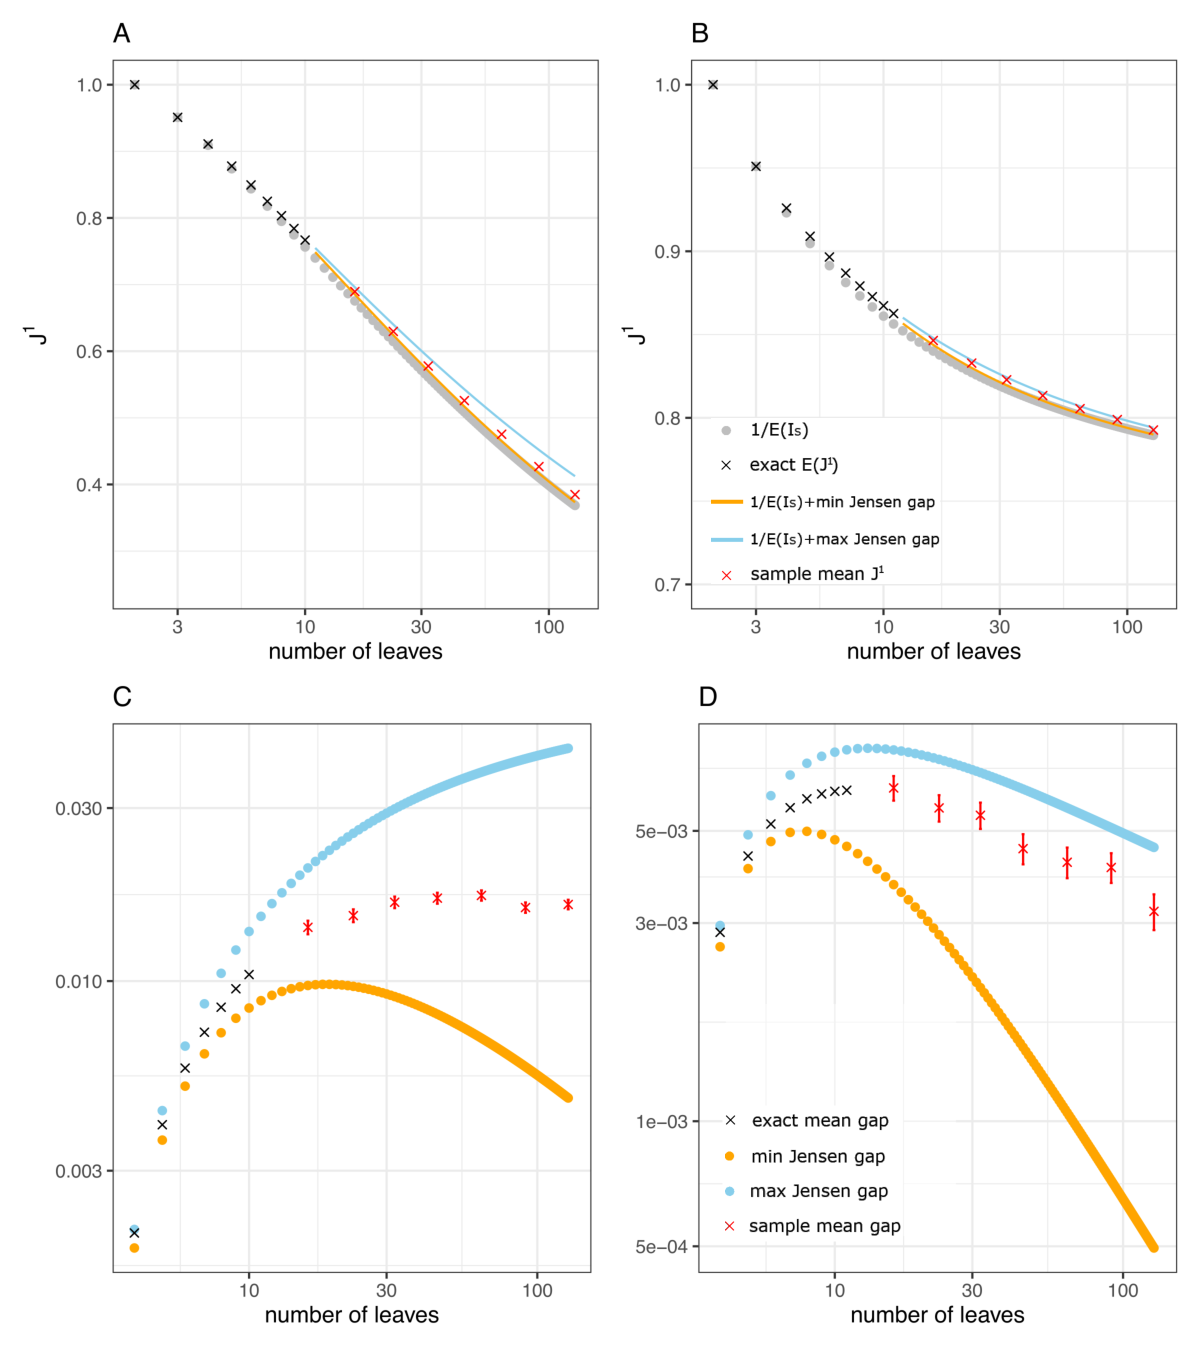
\includegraphics[width=\textwidth]{Chapter_2/figures/jensen_plots_final_edited.pdf}
    \caption{\textbf{Top row}: True values of $\mathbb E(J^1)$ for up to $10$
    leaves were calculated manually, and the approximations up to $128$ leaves
    were calculated as $n\log_2n/\mathbb E(I_S)$. \textbf{A} --- uniform model,
    \textbf{B} --- Yule model.\\
    \textbf{Bottom row}: The Jensen gap of $\mathbb{E}(J^1)$ calculated for
    trees up to $128$ leaves under the uniform model (\textbf{C}), and the Yule
    model (\textbf{D}). The size of the gap is calculated as the difference
    between the true and approximate expected value, with the gaps for $2$ and
    $3$ leaves equal to zero as there is only one possible bifurcating tree
    shape for each of those values. Refer to table \ref{table_values} for
    numerical values of the gap size for the first several values of $n$.
    The red crosses in \textbf{A} and \textbf{B} represent sample mean $J^1$
    values for $100000$ trees generated under the uniform model and Yule
    process, and the difference between the approximate gap size and the sample
    mean, with standard error represented by error bars, in \textbf{C} and
    \textbf{D}.}
    \label{jensenfig}
\end{figure}
\begin{figure}[h]
    \centering
    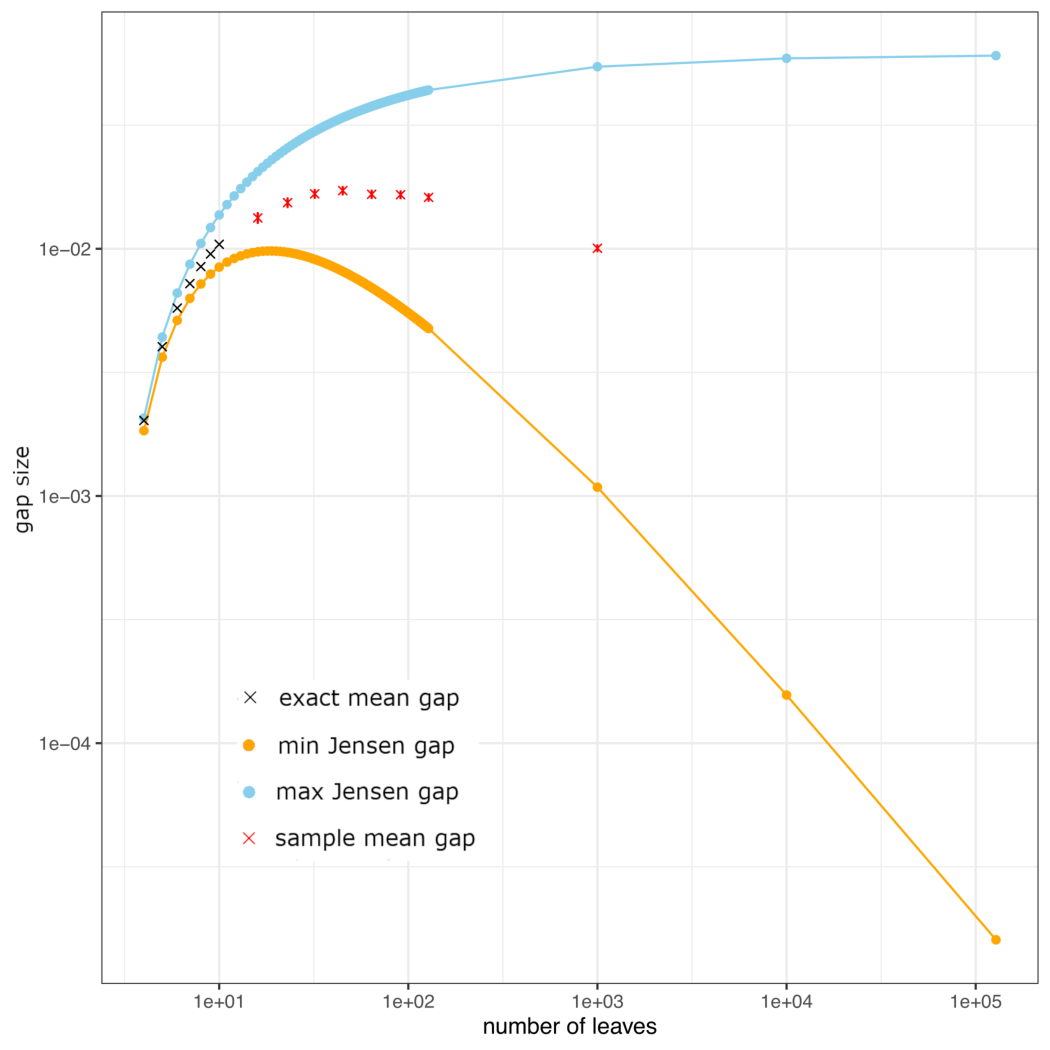
\includegraphics[width=\textwidth]{Chapter_2/figures/jensen_gap_1k.pdf}
    \caption{The convergence of the upper bound to $4/3\pi$ is much slower than
    the convergence of the lower bound to $0$, and the maximum it reaches over
    the plotted range is $0.0604$ for $n=128000$. The red crosses, as in figure
    \ref{jensenfig}, suggest convergence of the gap size.}
    \label{conv_upper_fig}
\end{figure}
\begin{figure}[h]
    \centering
    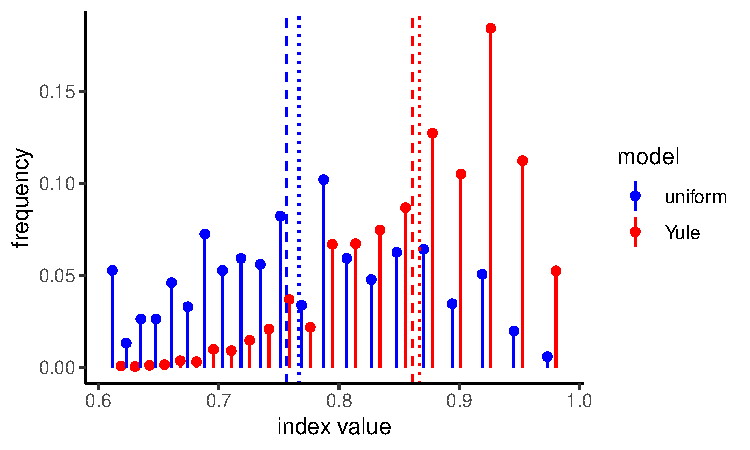
\includegraphics{Chapter_2/figures/var_fig.pdf}
    \caption{Higher variance in the uniform model leads to a non-zero upper
    bound on the Jensen gap. Shown are frequencies of $J^1$ values on $10$-leaf
    trees generated under the Yule and uniform models. The dashed lines
    represent the true expected value of $J^1$, and the dotted lines the
    approximate value calculated as $\frac{n\log_2n}{\mathbb{E}(I_S)}$}.
    \label{var_fig}
\end{figure}
\clearpage

The lower bound of $\mathbb{E}_U(J^1)-\frac{n\log_2n}{\mathbb{E}_U(I_S)}$ goes
to $0$ as $\frac{\log n}{n}$, while the upper bound tends to $\frac{4}{3\pi}$
for $n\to\infty$. This is a consequence of high variance in the uniform model
(figure \ref{var_fig}), as each tree on $n$ leaves is selected with equal
probability while the number of trees on $n$ grows exponentially with $n$,
the number of leaves. While I cannot prove analytically that the size of the
Jensen gap in this case tends to $0$, I can generate random trees using the
uniform model and compare the sample mean to the approximation using the
expected value of the Sackin index. In figure \ref{jensenfig}, I show behaviour
of the Jensen gap and its bounds for $J^1$ under the Yule and uniform models.
The red crosses in figures \ref{jensenfig}C and \ref{conv_upper_fig} indicate
that the gap size does converge for $n\to\infty$. Therefore, I propose the
following conjecture:

\begin{conjecture}
    For trees generated under the uniform model on $n\to\infty$ leaves, the
    following holds
    \begin{equation}
        \mathbb{E}_U(J^1) \to \frac{n\log_2n}{\mathbb{E}_U(I_S)}.
        \label{conjecture1}
    \end{equation}
\end{conjecture}

\begin{table}[h]
    \centering
    \begin{tabular}{|c|c|c|c|c|}
        \hline
        $n$ & $n\log_2n/\mathbb{E}_Y(J^1)$ & $\mathbb{E}_Y(I_S)$ & $n\log_2n/
        \mathbb{E}_U(J^1)$ & $\mathbb{E}_U(I_S)$\\
        \hline
        $2$ & $2$ & $2$  & $2$ & $2$ \\
        \hline
        $3$ & $5$ & $5$  & $5$ & $5$ \\
        \hline
        $4$ & $216/25$ & $26/3$ & $360/41$ & $44/5$ \\
        \hline
        $5$ & $728/57$ & $77/6$ & $3822/289$ & $99/7$ \\
        \hline
        $6$ & $1162800/67217$ & $87/5$ & $18.25643$ & $386/21$ \\
        \hline
        $7$ & $199806750/9017743$ & $223/10$ & $23.81979$ & $793/33$ \\
        \hline
        $8$ & $27.29901$ & $962/35$& $29.87282$ & $12952/492$\\
        \hline
        $9$ & $32.68993$ & $4609/140$ & $36.38201$ & $26333/715$ \\
        \hline
        $10$ & $38.30246$ & $4861/126$ & $43.31989$ & $106762/2431$ \\
        \hline
        $11$ & $44.11464$ & $55991/1260$ & n/a & n/a \\
        \hline
    \end{tabular}
    \caption{Comparison of exact and approximate expected values of $J^1$ and
    $I_S$ under the Yule and uniform models.}
    \label{table_values}
\end{table}

\subsection{Analytic properties of the $J^1$ index}
The index $J^1$ is normalised in a way which makes comparison of its values on
trees of different sizes valid \citep{lemant_robust_2022}. As $J^1$ was defined
to take into account node sizes, it can take any value between $0$ and $1$ for
any given tree topology (figure \ref{balcat}). Furthermore, since $J^1$ is
defined to be $0$ on linear trees, finding its minimal value on a given number
of nodes is trivial. In this section I investigate extremal values on trees
where I impose restrictions to both topology and node size distributions, i.e.
consider only leafy trees with out-degree of each internal node greater than $1$.

\begin{figure}[h]
    \centering
    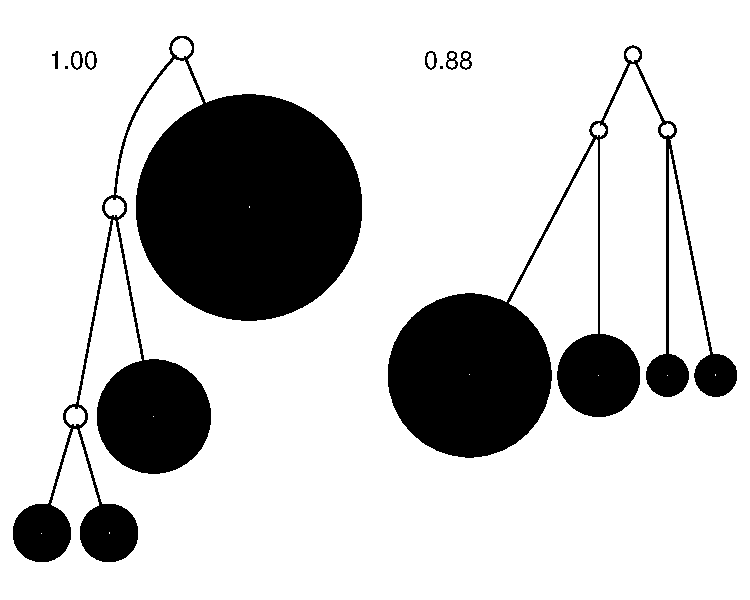
\includegraphics[width=0.8\textwidth]{Chapter_2/figures/balcat.pdf}
    \caption{By including the node-balance function $W^1$ in $J^1$, we allow for
    the possibility of perfectly balanced caterpillars (left) and less balanced
    fully symmetric trees (right) based on the node size distribution in the
    tree. The leaf sizes in these two trees are identical, with a ratio
    $4:2:1:1$ from largest to smallest.}
    \label{balcat}
\end{figure}

\subsection{Properties of $J^1$ on different tree families}

For most balance indices in use in evolutionary biology, the least balanced tree
for a given number of leaves $n$ is the binary caterpillar tree. I have
previously derived a general expression for leafy trees of this topology
\citep{lemant_robust_2022}
\begin{equation}
    J^1(T_C) = \frac{2n\log_2n}{(n-1)(n+2)}.\label{caterpillar}
\end{equation}
Most balance indices in literature define the caterpillar topology as the least
balanced one \citep{fischer_tree_2021}. Intuitively, this makes sense as balance
is often associated with symmetry, and the caterpillar is the most asymmetric
bifurcating tree. However, in the context of the $J^1$ index, tree topology is
just one of a few factors which contribute to the balance score of a tree,
especially since the index does not limit the space of trees to bifurcating ones.
Also important to consider are node sizes and, more specifically, how the population
is split across different subtrees in the tree of interest. Let us consider a
slightly altered caterpillar topology. \par

\begin{figure}[h]
    \centering
    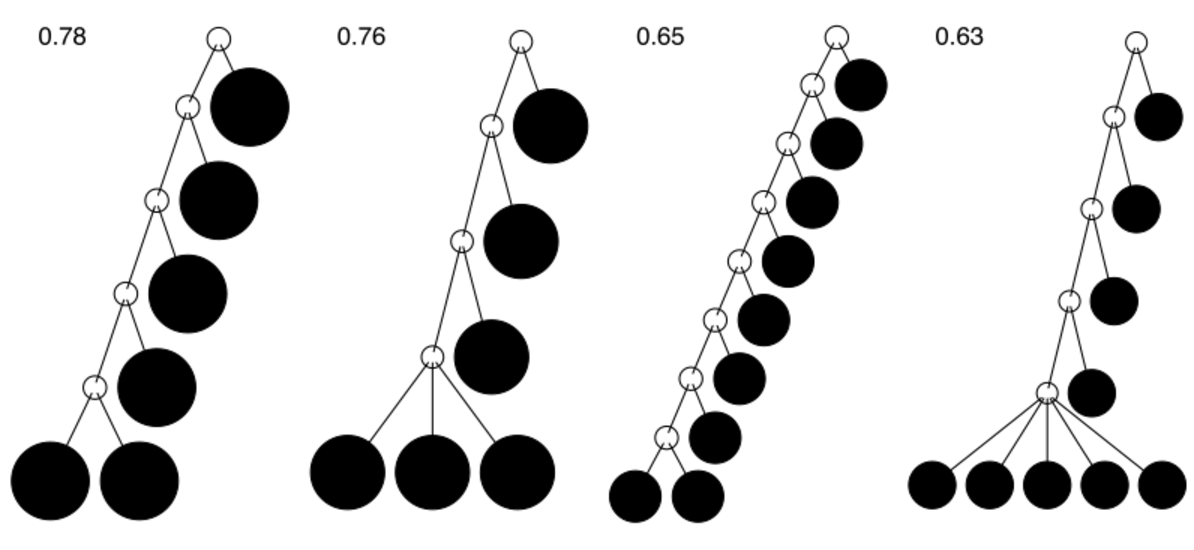
\includegraphics[width=\textwidth]{Chapter_2/figures/example_figure_1.pdf}
    \caption{If we limit our search to leafy trees with equal leaf sizes, the
    least balanced tree on a given number of leaves is not necessarily the
    caterpillar. Pictured are the caterpillar trees on $6$ and $9$ leaves, as
    well as minimally balanced brooms for $6$ and $9$ leaves,
    with corresponding $J^1$ values.}
    \label{example_figure_1}
\end{figure}

\begin{definition}
    Let $T_B$ be a leafy tree on $n$ leaves. Let every internal node of $T_B$
    except for the most distant one from the root have out-degree $2$ such that
    one of its descendants is a leaf, and the other an internal node. Further,
    let the internal node most distant from the root have out-degree $k$.
    Then we call tree $T_B$ a \textbf{broom tree}.\\
    We call the leaves attached to the internal node with the highest out-degree
    the \textbf{broom head}, and the remaining leaves are attached to the \textbf{handle}.
\end{definition}
A general expression of $J^1$ for this family of trees is then derived.
\begin{proposition}\label{broom_prop}
    The value of $J^1$ for a broom tree $T_B$ on $n$ leaves, of which $k$ in the broom head is
    \begin{equation}
        J^1(T_B) = \frac{2\left( n \log_2 n - k \log_2 k + k \right)}{(n+k)(n-k+1)}.\label{J1Tb}
    \end{equation}
\end{proposition}
\begin{proof}
    \begin{align*}
        J^1(T_B) &= \frac{1}{\sum_{l=k}^{n}l} \sum_{i\in\tilde{V}} S_i^{*}
        \sum_{j\in C(i)}W_{ij}^{1}\\
        &= \frac{-2}{(n+k)(n-k+1)}\sum_{i \in \tilde{V}} S_i^*\sum_{j\in C(i)}
        \frac{S_j}{S_i^*}\log_{d^+(i)} \frac{S_j}{S_i^*}\\
        &=\frac{-2}{(n+k)(n-k+1)}\left(\sum_{\substack{i \in \tilde{V}\\d^+(i)=2}}
        S_i^*\sum_{j\in C(i)} \frac{S_j}{S_i^*}\log_2\frac{S_j}{S_i^*}+k\cdot
        k\cdot\frac{1}{k}\log_k \frac{1}{k}\right)\\
        &= \frac{-2}{(n+k)(n-k+1)}\left(\sum_{\substack{i \in \tilde{V}\\d^+
        (i)=2}} S_i\left(\frac{S_i-1}{S_i}\log_2\frac{S_i-1}{S_i}+\frac{1}{S_i}
        \log_2\frac{1}{S_i}\right)-k\right)\\
        &= \frac{2}{(n+k)(n-k+1)}\left( \sum_{i=k+1}^{n} i\left( \frac{i-1}{i}
        \log_2\frac{i}{i-1}+\frac{1}{i}\log_2 i \right)+k \right)\\
        &= \frac{2}{(n+k)(n-k+1)}\left(  \sum_{i=k+1}^{n}\left( (i-1)\log_2
        \frac{i}{i-1}+\log_2 i \right) +k \right)\\
        &= \frac{2}{(n+k)(n-k+1)}\left( log_2\frac{n^n k!}{k^k n!}+\log_2
        \frac{n!}{k!}+k \right)\\
        &= \frac{2}{(n+k)(n-k+1)}\left( \log_2\frac{n^n}{k^k}+k \right)\\
        &= \frac{2}{(n+k)(n-k+1)}\left( n \log_2 n - k \log_2 k + k \right)
    \end{align*}
\end{proof}

The result of proposition \ref{broom_prop} is directly generalisable in the
following way.

\begin{proposition}\label{q-broom-prop}
    For a broom tree $T_{Bq}$ on $n$ leaves, of which $k$ in the broom head,
    such that the sizes of leaves in the head sum to $q\in \mathbb R$, and the
    leaves in the handle all of equal size $1$, the value of $J^1$ is
    \begin{align*}
        J^1(T_{Bq}) &= \frac{1}{(n-k+1)(q+(n-k)/2)}\\
        &\times\left( q\log_k q-\left(\sum_{i=1}^{k}l_i\log_k l_i\right)+(q+n-k)
        \log_2(q+n-k) - q\log_2q \right),\numberthis\label{J1Tbq}
    \end{align*}
    where $l_1,\dots,l_k$ are the leaf sizes which add up to $q$.
\end{proposition}

In figure \ref{example_figure_1} I show that the caterpillar is not the
minimally balanced leafy tree for a few tree sizes. To take it a step further,
consider the following proposition.

\begin{proposition}\label{cat_prop}
    For leafy trees on $n$ leaves and no linear parts, the caterpillar minimises $J^1$ iff $n<5$.
\end{proposition}

\begin{proof}
    Let $J^1_B(n,k)$ denote the value of $J^1$ on a broom tree with $n$ leaves,
    of which $k$ in the broom head. Then
    \begin{align}
        J^1_B(n,2) = & \frac{2n\log_2n}{(n+2)(n-1)}, \label{j1bn2}\\
        J^1_B(n,3) = & \frac{2}{(n+3)(n-2)}(n\log_2n - 3\log_2 3 + 3).\label{j1bn3}
    \end{align}
    Consider the case when $J^1_B(n,2) < J^1_B(n,3)$. Plugging in equations
    \eqref{j1bn2} and \eqref{j1bn3}, we can rearrange the inequality to find
    \begin{equation}
        8n\log_2n - 6(n^2+n-2)\log_2 3 + 6(n^2+n-2) > 0,
    \end{equation}
    which changes sign at $0, 0.667, 1$ and $4.168$. Setting the first
    derivative of this expression to zero
    \begin{equation*}
        8\log_2n+\frac{8}{\log 2}-(12n+6)\log_2 3 + 12n + 6 = 0
    \end{equation*}
    we find solutions around $n=0.822$ and $n=2.888$, the latter of which
    signifies a local maximum. Therefore, as $n$ can only take positive integer
    values, valid solutions for which the caterpillar is less balanced than the
    broom with $3$ leaves in the broom head according to the index $J^1$ are $3$
    and $4$, with the $k=3$ broom being less balanced otherwise.
\end{proof}

This proposition gives us a threshold for the number of leaves at which the
caterpillar is no longer the minimally balanced tree for the given number of
leaves, which sets $J^1$ apart from conventional balance indices (figure
\ref{Rfigures}A). However, I am yet to prove the following statement.

\begin{conjecture}\label{conj}
    For leafy trees on $n$ leaves and no linear parts, the tree that minimises
    $J^1$ belongs to the broom family.
\end{conjecture}

\subsection{Behaviour as $n\to\infty$}

\begin{figure}[h!]
    \begin{center}
    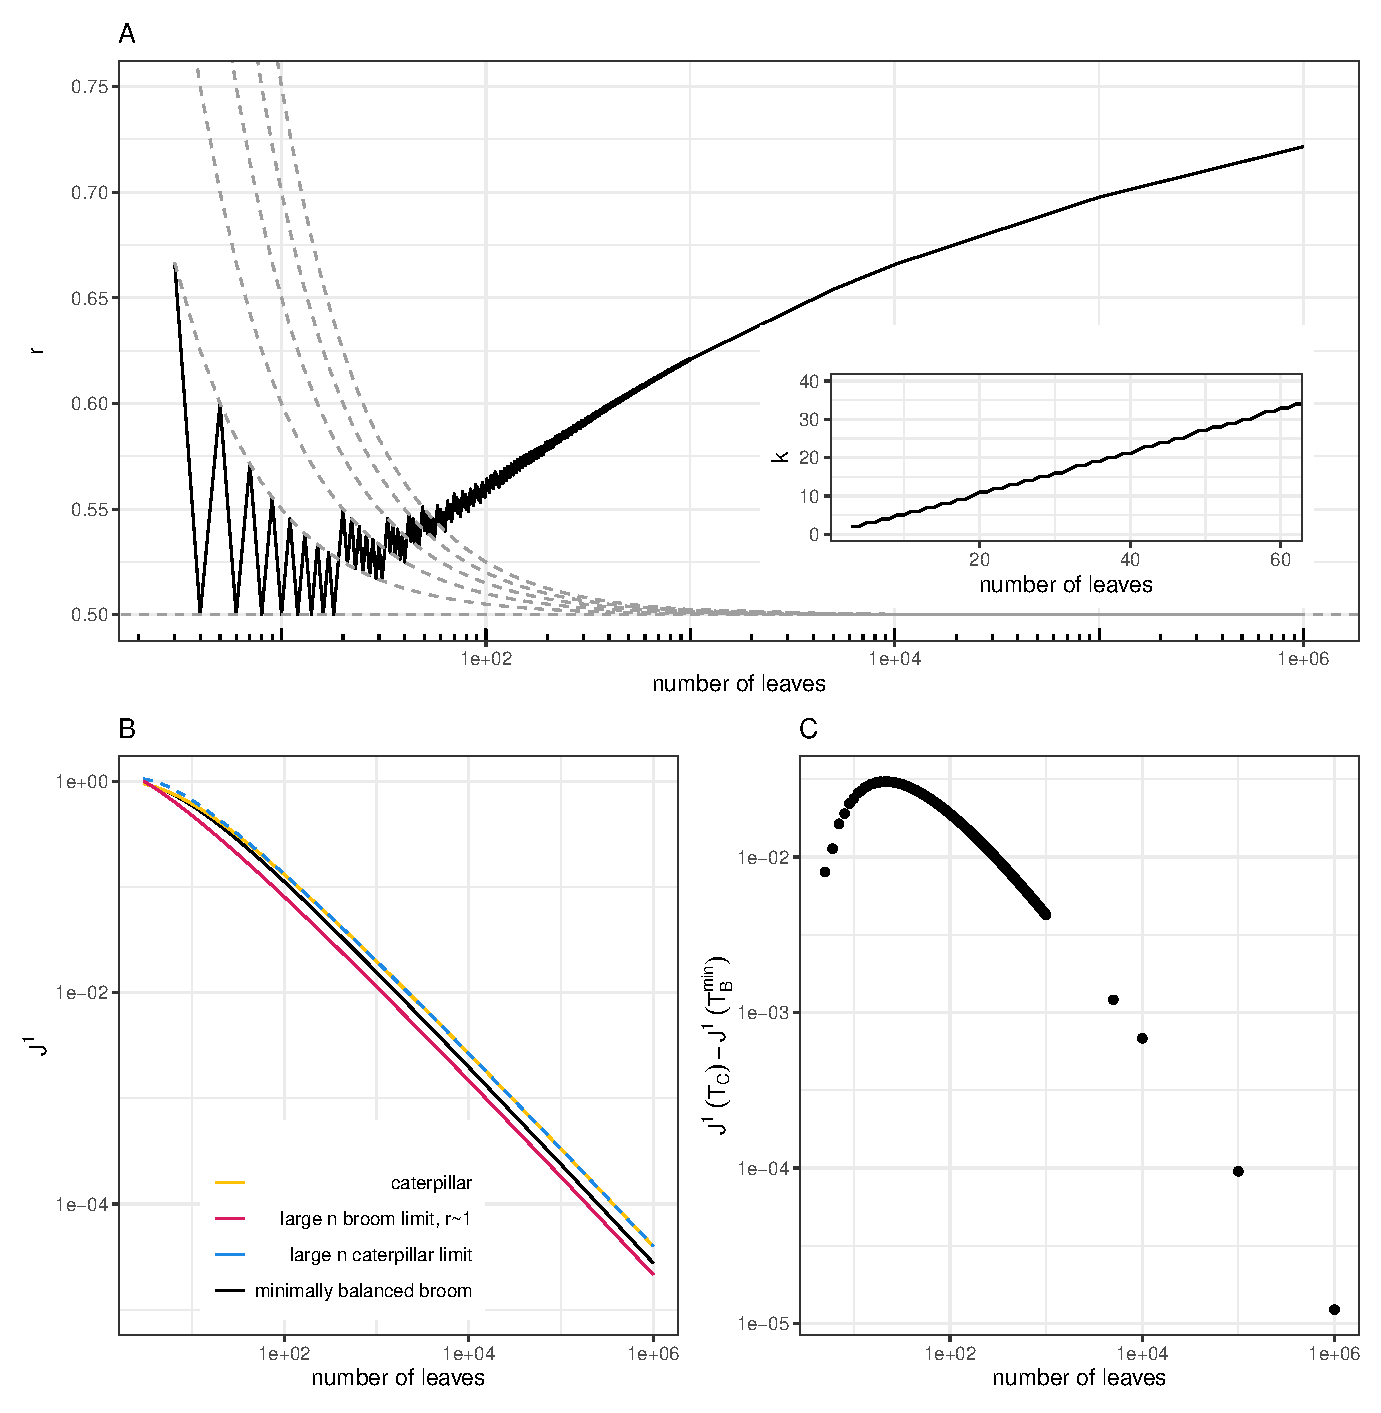
\includegraphics[width = \textwidth]{Chapter_2/figures/j1_figure_3_plots.pdf}
    \caption{The labels used in the figures are as above - $n$ for number of
        leaves, $k$ for number of leaves in the broom head, $r=n/k$.
        \textbf{A:} Value of $r$ for which the minimum value of $J^1$ is
        obtained on leafy trees. Trees on $n$ leaves which satisfy
        $r = \frac{n+a}{2n}$, for $a=0,1,2,\dots$ lie on the dashed grey lines.
        The inset plot shows $k = rn$, the number of leaves attached at the
        broom head. \textbf{B:} Comparison of true and approximate values of
        $J^1$ for the caterpillar and minimally balanced broom trees as a
        function of $n$. \textbf{C:} The difference between values of $J^1$ of
        the minimally balanced broom and the caterpillar trees.}
    \label{Rfigures}
    \end{center}
\end{figure}
\clearpage

I have derived general behaviour of $J^1$ on broom and caterpillar trees for a
given number of leaves $n$, showing that caterpillar trees are not necessarily
minimally balanced for a given number of leaves. If we let $n\to\infty$, the
value of $J^1$ for the caterpillar from equation \eqref{caterpillar} will
behave like
\begin{equation}
    \lim_{n\to\infty} J^1(T_C) = \frac{2\log_2n}{n}. \label{caterpillarlim}
\end{equation}
As $J^1$ is not limited to trees with equal leaf sizes, there is a threshold we
can impose on the broom tree beyond which the caterpillar is less balanced.

\begin{proposition}\label{p-broom-prop}
    Let $T_B(n)$ be a broom tree on $n$ leaves such that the leaves on the
    handle and head have sizes $f$ and $fp$ respectively, and $T_C(n)$ be a
    caterpillar tree on $n$ leaves of equal sizes $f$. Then
    \begin{equation}\label{p-broom-cond}
        J^1(T_B) > J^1(T_C) \text{\quad iff \quad} p<\frac{1}{2},
    \end{equation}
    as $n\to\infty$.
\end{proposition}
\begin{proof}[Proof of proposition \ref{p-broom-prop}]
    Let $n\to\infty$. The the value of $J^1$ for the caterpillar tree tends to
    \begin{equation*}
        J^1(T_C) = \frac{2\log_2n}{n},
    \end{equation*}
    and for the broom tree with equally sized leaves of size $p$ in the broom head
    \begin{equation*}
        J^1(T_{B,p}) = \frac{2}{n(1-r)(1+r(2p-1))}\left[ (r(p-1)+1)\log_2
        n(r(p-1)+1) - rp\log_2 nrp \right].
    \end{equation*}
    We can evaluate the difference between these expressions:
    \begin{align*}
        J^1(T_C) - J^1(T_{B,p})  \sim &  (1-r)(1+r(2p-1))\log_2n+rp\log_2nrp \\
        & - (r(p-1)+1)\log_2n(r(p-1)+1) \\
        \sim & ((1-r)(1+r(2p-1))-(r(p-1)+1)+rp)\log_2n + o(\log_2n).
    \end{align*}
    The difference is dominated by the term containing $\log_2n$ which is always
    positive. The term in the brackets preceding it can be negative, however:
    \begin{equation*}
        (1-r)(1+r(2p-1)) - r(p-1) + 1 + rp = r(1-r)(2p-1).
    \end{equation*}
    As $r = k/n$, with $k$ the number of leaves in the broom head, it is always
    positive. Thus, the expression is negative only when $2p-1<0$ or $p<\frac{1}{2}$
\end{proof}

\begin{figure}[h!]
    \centering
    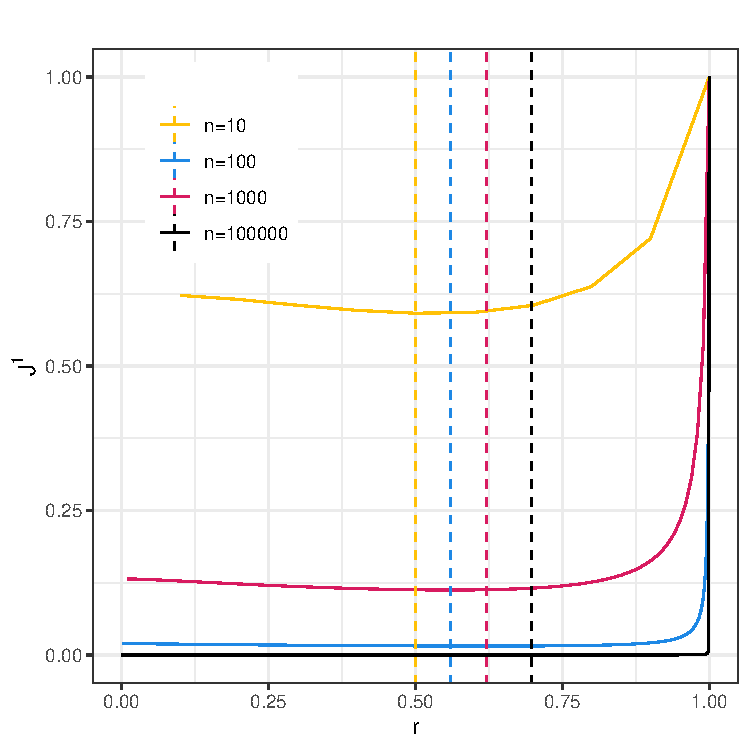
\includegraphics[width=.7\textwidth]{Chapter_2/figures/j1_lines_plot.pdf}
    \caption{Values of $J^1$ on trees of different sizes calculated using
    equation \eqref{J1Tb} for different values of $r=k/n$. The dashed lines are
    at values of $r$ which minimise $J^1$.}
    \label{j1_lines_plot}
\end{figure}

For broom trees, the behaviour is a little more complicated and, perhaps,
counter-intuitive (figure \ref{j1_lines_plot}). Consider the following.

\begin{proposition}\label{ropt_prop}
    Let $\mathcal{T}_B(n)$ be the set of all leafy broom trees with equal leaf
    sizes on $n$ leaves, $r = \frac{k}{n}$ where $k$ is the number of leaves in
    the broom head for a given tree, and $r_\text{opt}$ the value of $r$ which
    minimises $J^1$ for a given $n$. Then $r_\text{opt}\to 1$ as $n\to\infty$.
\end{proposition}
\begin{proof}
    Let $r = k/n$ and $J^1_B(n,r)$ the value of $J^1$ for a broom tree on $n$
    leaves, of which $k$ in the head. Then
    \begin{equation}
        J^1 \stackrel{n\to\infty}{=} \frac{2}{n(1-r)(r+1)}((r+1)\log_2n(r+1)-
        r\log_2nr)
        \label{broomlim}
    \end{equation}
    which is minimised for $r\to1$.
\end{proof}

The proposition says that most leaves on a minimally balanced broom tree will be
concentrated in the head, with comparatively few on the handle, resembling a
star tree more closely than a caterpillar tree. However, one must take into
account how imbalanced the nodes above the broom head are, since one of their
subtrees contains most of the tree's leaves, whereas the other is a single leaf.
For practical purposes, the difference between the $J^1$ values of the minimally
balanced broom and the caterpillar for the number of leaves $n\to\infty$ is
small and decreases rapidly as $n$ grows (figure \ref{Rfigures}B,
\ref{Rfigures}C). \par
Finding the true value of $k$ which minimises $J^1(T_B)$ analytically is
difficult. The derivative with respect to $k$ of equation \eqref{J1Tb} yields a
transcendental equation which is not analytically solvable. I also cannot
analytically determine whether broom trees minimise $J^1$ for a given number of
leaves. However, I have exhaustively checked whether the broom minimises $J^1$ up
to $12$ leaves --- which it does. Beyond that, the number of possible trees
grows too rapidly for a similar verification to be computationally feasible
without an efficient tree generating algorithm for trees with arbitrary node
degree distributions.

\section{Discussion}
The aim of this chapter was to explore deeper analytic properties of the universal
balance index $J^1$ and carve its place in the broader context of tree balance
by extending past results and uncovering new connections. \par
In the chapter I focussed on trees with uniform branch lengths, as $J^1$ was not
defined with them under consideration. A further generalisation of metric
describing tree properties is therefore the logical next step
\citep{noble_new_2023}. \par
I calculated an approximate expectation of $J^1$ under the most common null
models used in evolutionary biology. Having a good approximation for the
expected value of $J^1$ is a crucial result in the development of this index,
as it allows us to employ it in the analysis of evolutionary processes on
phylogenetic trees. The next step in this direction would be to obtain a
closed-form solution for the expectation of $J^1$, as well as its variance.\par
Finally, I only touched upon directly obtainable relationships without
considering different real-world use cases of the index and the implications of
equation \eqref{prop6}. This is another avenue of future research as there may
exist a relationship between the way indices vary with time and the underlying
evolutionary process growing the associated tree.


\chapter{Tracking cancer evolution \textit{in silico} via evolutionary indices}
\textit{A part of the results from this chapter were presented in poster form at MMEE 2022 in Reading and at ECMTB 2022 in Heidelberg.}

\section{Introduction}
A trajectory is a path described by any object (or indeed point) in some space according to some parameter, usually time.  Intuitively then, an evolutionary trajectory refers to the changes that a lineage or population undergoes over time --- the series of genetic, morphological, and behavioral transformations that occur as organisms evolve and diversify. We are interested in the evolutionary trajectory of cancers but reliably obtaining time-series data is, at the time of writing, not feasible at a larger scale. This stems from multiple issues. Firstly, at time of diagnosis, solid tumours have likely already been growing for long enough to reach a size visible in standard medical imaging \cite{patrone_how_2011}. This means that even initial data obtained in the clinic represents a relatively late stage in the cancer's evolutionary history most of the time. Secondly, solid tumours are just that --- clumps of cells organised in some way in space --- meaning that taking a sample from one point in the tumour is not necessarily representative of the rest of the cell population. Finally, a biopsy is an invasive procedure which can cause considerable discomfort to patients, depending on where the tumour is situated. Therefore, having a reasonable estimate of a tumours evolutionary trajectory based on the data that is available at time of sequencing would allow for a more informed treatment strategy.\par
In this chapter, we will exmine the utility of two different sets of evolutionary indices for tracking the evolution of tumours \textit{in silico}.

\subsection{Why even bother with indices?}
Before introducing the sets of indices used to analyse properties of trees, let us consider a simpler question --- can we map the set of all possible trees to the set of real numbers? For this purpose we should decide how to define the set of trees. The number of nodes in a tree is a natural number, $n\in\mathbb{N}$, as is the number of possible tree topologies for a given $n$. We denote with $T(n)$ the set of enumerated tree topologies \cite{nakano_tree_2016}. Each node then has a corresponding size, giving us an $n$-tuple of real numbers $(\alpha_1, \dots, \alpha_n)\in\mathbb{R}^n$, and each edge (branch) has a corresponding length or $(l_i, \dots, l_{(n-1)})\in\mathbb{R}^{(n-1)}$. This means we would need a family of maps
\begin{equation}
    f_n: A(n) \times \mathbb{R}^n \times \mathbb{R}^{n-1} \rightarrow R.
\end{equation}
It would be easy to construct a mapping which would allow us to ``enumerate" each possible tree with a real number. The only problem with this approach is that it is not at all useful, first and most importantly due to its lack of any interpretability. This chapter outlines an approach which uses real-valued summaries of trees' properties in a way that is both intuitive and mathematically sound.

\subsection{A 3-dimensional index space --- trees with uniform branch lengths}
\subsubsection{Shannon diversity}
Shannon entropy is a fundamental concept in information theory, that quantifies the uncertainty or randomness of a system \cite{shannon_mathematical_1948}. By considering a system where diversity represents the variety of elements, such as intra-tumour heterogeneity, we can define the Shannon diversity as the exponential of the Shannon entropy,
\begin{equation}
    \leftindex[I]^1{D} = \exp\left[\leftindex[I]^1{H}\right] = \exp\left[-\sum_{i=1}^N p_i \log p_i\right],
\end{equation}
where $N$ is the total number of categories (or elements, species, etc.), and $p_i$ the frequency of category $i$. The Shannon diversity was chosen because of the nice property that it is maximised and equal to the number of categories when all categories are equally represented, and minimised when only one category is present.
\subsubsection{Mean number of drivers per cell --- distance from the root}
Each speciation event in phylogenetics or driver mutation in cancer evolution is associated with a change in the corresponding tree's topology. To capture the average number of these events, we use the mean number of drivers per cell. This is defined as the average of distances from all nodes to the root (with the root distance from itself defined as $1$) weighted by the frequencies of the subclones,
\begin{equation}
    n = \sum_{i=1}^N p_i \nu(i),
\end{equation}
where $\nu(i)$ is the root distance of node $i$.
\subsubsection{Balance index}
As discussed in chapter \ref{chapter:indices}, the balance index $J^1$ is a weighted average of the evenness of the population distribution within a tree. We use it as the third index in this space.

\subsection{A general set of indices --- any rooted tree}
Expanding upon the $3$-dimensional space defined above, a new comprehensive set of interpretable robust indices based on Hill numbers was introduced recently \cite{noble_new_2023}. The authors expanded and improved upon the existing quantifiers of tree shape properties by deriving methods for trees with arbitrary node size, node degree, and branch length distributions. The methods for calculating all of the indices are included as part of an R package \cite{kimverity_kimverityruiindices_2023}.\par
Each generalised index has three components, depending on which part of the tree it is applied --- the longitudinal mean, node-wise mean, star mean.
\subsubsection{Richness --- $\leftindex[I]^0{D}$}
Richness in the context of phylogenetics is simply the number of extant species, i.e. the number of tips in a phylogenetic tree. The generalised richness's three components are:
\begin{enumerate}
    \item $\leftindex[I]^0{D}_L$ --- the average number of branches across the tree;
    \item $\leftindex[I]^0{D}_N$ --- the average effective outdegree, ignoring branch sizes;
    \item $\leftindex[I]^0{D}_S$ --- the effective number of non-root nodes.
\end{enumerate}
\subsubsection{Diversity --- $\leftindex[I]^q{D}$, $q>0$}
The generalised diversity index represents an extension of the Shannon diversity index. Its three components are:
\begin{enumerate}
    \item $\leftindex[I]^q{D}_L$ --- the effective number of maximally distant nodes (leaves);
    \item $\leftindex[I]^q{D}_N$ --- the average effective outdegree, accounting for branch sizes, i.e. bushiness;
    \item $\leftindex[I]^q{D}_S$ --- the effective numbering of branches, accounting for branch sizes.
\end{enumerate}
\subsubsection{Evenness --- $\leftindex[I]^q{J}$, $q>0$}
Finally, the extension of the robust universal balance index $J^1$, this set of indices generalises tree balance in the following way:
\begin{enumerate}
    \item $\leftindex[I]^q{J}_L$ --- evenness of branch sizes across the tree, or tree symmetry for leafy and ultrametric trees;
    \item $\leftindex[I]^q{J}_N$ --- tree balance, or evenness of the node size distribution;
    \item $\leftindex[I]^q{J}_S$ --- evenness of all branch sizes.
\end{enumerate}

\section{Tree resolution}
% \begin{itemize}
%     \item using numerical summaries may sound reasonable, but does it produce distinct enough results?
%     \item what is the minimal number of indices we need to consider to tell apart two trees in general
%     \item how about in the context of realistic data (e.g. driver trees)?
% \end{itemize}
The first question we need to address is whether the indices we have chosen are sufficient to distinguish between different trees.
\subsection{3-dimensional index space}
% \begin{itemize}
%     \item we begin by examining the simplest case - leafy trees with equal leaf sizes
%     \item consider first the smaller set of indices ($J^1$, $D_{Shannon}$, $N_{drivers}$)
%     \item in this case we can construct a family of trees based on the canonical factorisation of $n$, the number of leaves
%     \item then show what this looks like on the expanded set of indices (Rob \& Kim)
%     \item all of these trees are perfectly balanced and symmetric, making them an unlikely appearance in real data (cite data papers to show what real data looks like, e.g. TracerX)
%     \item loosening up our criteria for what a tree looks like we consider leafy trees with arbitrary node sizes
%     \item can again construct artificial examples for the smaller set of indices
%     \item more difficult for the expanded set
% \end{itemize}
Starting simple, we examine leafy trees with all leaves of equal size in the $3$-dimensional index space. The first thing to note is that the Shannon diversity will simply equal the number of leaves in the tree. This already takes away a degree of freedom. The next thing to consider is the value of $J^1$. If we limit our search, for now, to perfectly balanced trees, we are left with symmetric trees on a fixed number of leaves $N$. To make the final index equal between two trees, they need to have equal average depths of their leaves. As we are only looking at perfectly symmetric trees, that means that the average depth will be exactly equal to the individual leaf depths. We can then show the following
\begin{proposition}
    Let $T$ be a symmetric leafy tree on $N$ leaves with equal leaf sizes. If the canonical factorisation of $N$ is
    \begin{equation}
        N = \prod_{i=1}^k \alpha_i^{l_i},
    \end{equation}
then there are $k$ distinct trees with the same values of $J^1$, $\leftindex[I]^1{D}$, and $n$, including $T$.
\end{proposition}
\begin{proof}
    $\dots$
\end{proof}

\section{Computational methods}
\subsection{Agent-based modelling framework - \textit{warlock/demon}}
There is no shortage of agent-based models of tumour evolution \cite{colyer_seven-step_2023}, and the can range from purpose-built complex frameworks to more stripped-down and abstract ones. Since each model should be ``as simple as possible but no simpler", the appropriate framework for our purposes must satisfy certain requirements --- flexibility, efficiency, and reproducibility. The first requirement is deceptively specific. As the main inspiration behind this work stems from cancer evolution, we want our simulations to have parameters for controlling aspects of the cell population's physical properties which would in turn imply a different way in which it evolves. This would, for example, include spatial arrangement of cells, mutation rates, migration rates, and selective advantage. Furthermore, while the goal is to simulate large populations of cells, we also need a large number of simulations over which we can infer more general deterministic properties. Stochastic effects could make vastly different evolutionary modes look more similar than expected in theory. Finally, reproducibility allows us to share parameters of our models for verification by peers, and possible further investigation.\\
The agent-based modelling framework we decided to use is \texttt{warlock} \cite{bak_warlock_2023}, a \texttt{snakemake} wrapper written for \texttt{demon} \cite{noble_demon_2020}. It satisfies the requirements above, with a few associated comments. Firstly, it is a flexible agent-based model of tumour evolution as it does have parameters which control for spatial arrangement, mutation rates and selective advantage, as well as migration. While it is able to simulate spatial structure, \texttt{demon} covers at most two spatial dimensions. This is not an issue since we approximate the cell population to undergo stochastic isotropic growth, that is the tumour has equal probability of expanding in all directions in space. This implies approximate spherical symmetry of simulated solid tumours, which allows us to effectively consider the two-dimensional simulation as a cross-section of a tumour spheroid. In terms of efficiency, \texttt{demon} was written mainly in C++, and conceptualised so that instead of tracking individual cells, it simulates unique cell genotypes on a two-dimensional grid comprised of demes, or well-mixed patches of cells. The procedure for simulation cell events is based on the Gillespie algorithm \cite{gillespie_exact_1977}, and follows the steps of selecting a deme, then cell type, event type, and finally cell genotype. This approach sacrifices micro-scale interactions between cells to benefit efficiency and the feasibility of mathematical analysis of the model using, for example, diffusion approximations. Finally, all associated code is free and open source (cite github repos once finished), which allows reproducibility using identical parameters and random seeds. Parameter values for different batches can be found in the appendix (ref).


\section{Results}
\subsection{Sensitivity of evolutionary mode to parameter values}
\begin{itemize}
    \item there is clear variance in trajectories within a spatial config but less than one might expect for parameters within an order of magnitude of each other
    \item all things but spatial config being equal, the trajectories seem to be distinct in later stages of evolution
    \item should formalise somehow??
\end{itemize}
\begin{figure}
    \centering
    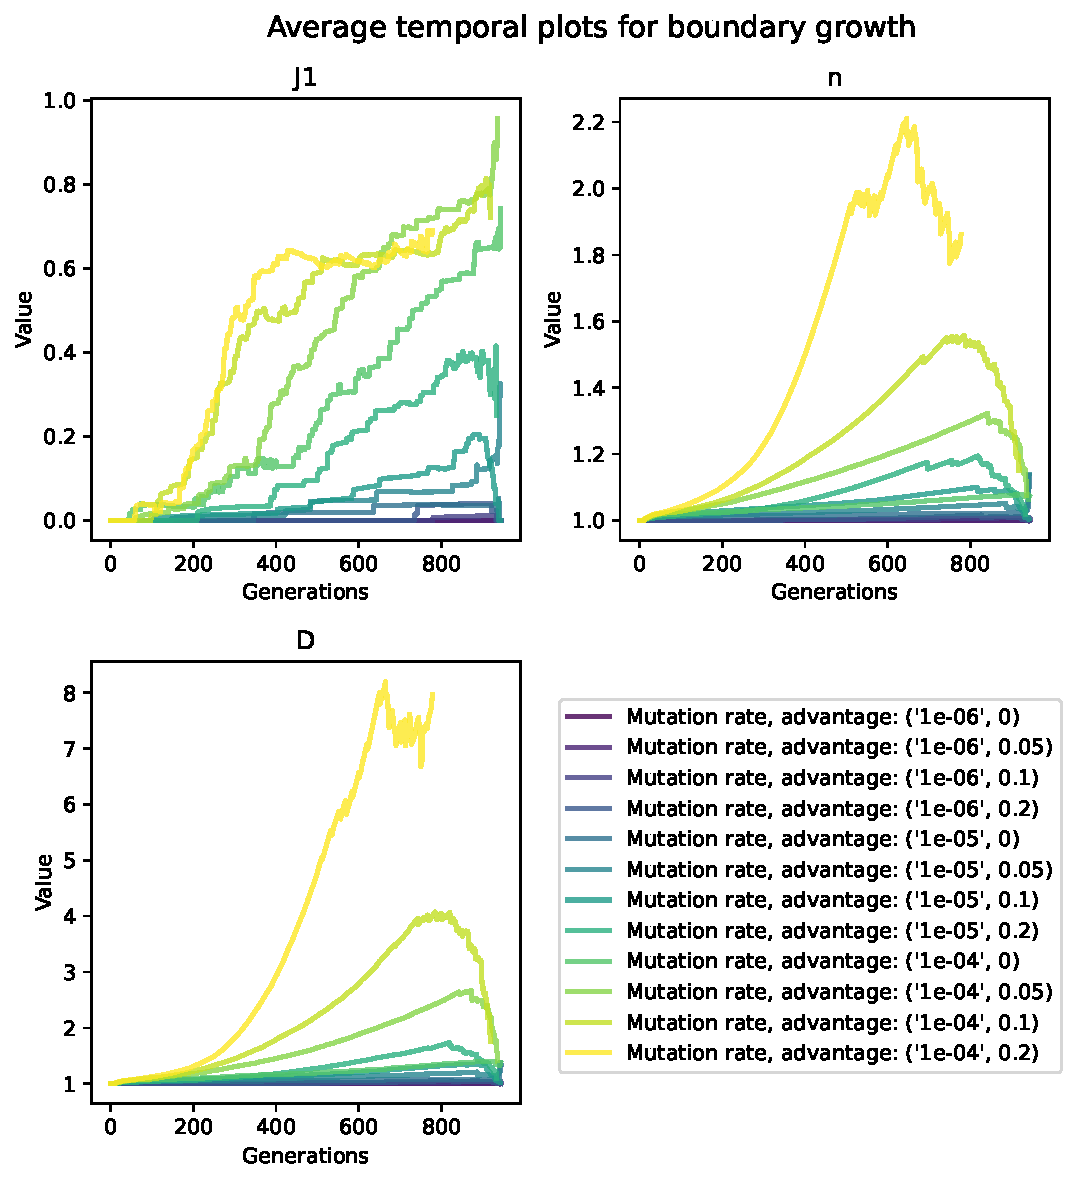
\includegraphics[width=\textwidth]{Chapter_3/figures/boundary-temporal.pdf}
    \caption{Average trajectories of the three indices for different values of driver mutation rate and selective advantage for tumours progressing via boundary growth.}
    \label{fig:boundary-temporal}
\end{figure}
\begin{figure}
    \centering
    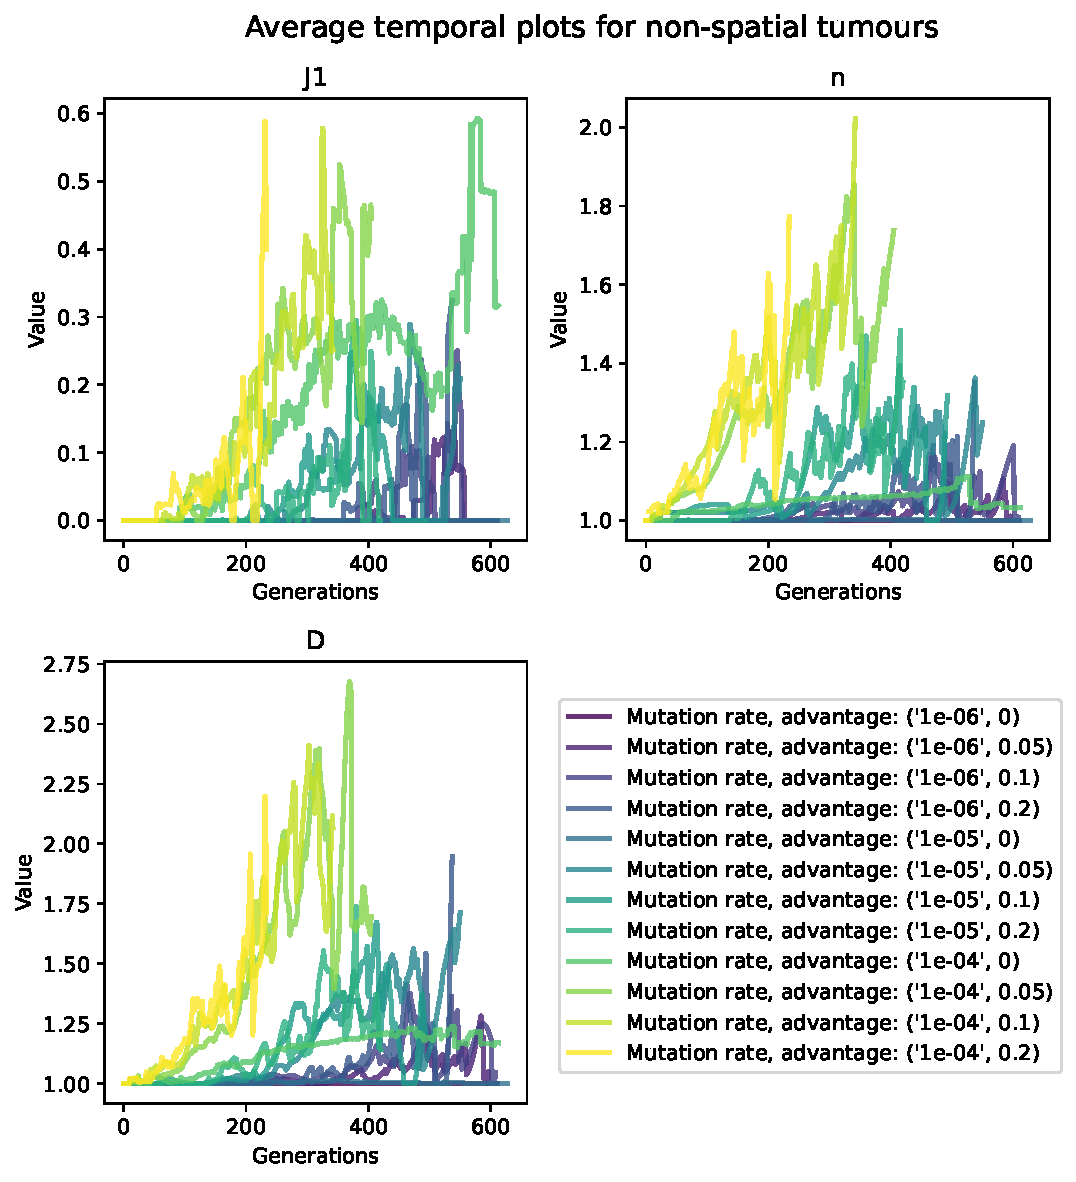
\includegraphics[width=\textwidth]{Chapter_3/figures/non-spatial-temporal.pdf}
    \caption{Average trajectories of the three indices for different values of driver mutation rate and selective advantage for well-mixed cancer cell populations.}
    \label{fig:non-spatial-temporal}
\end{figure}
\begin{figure}
    \centering
    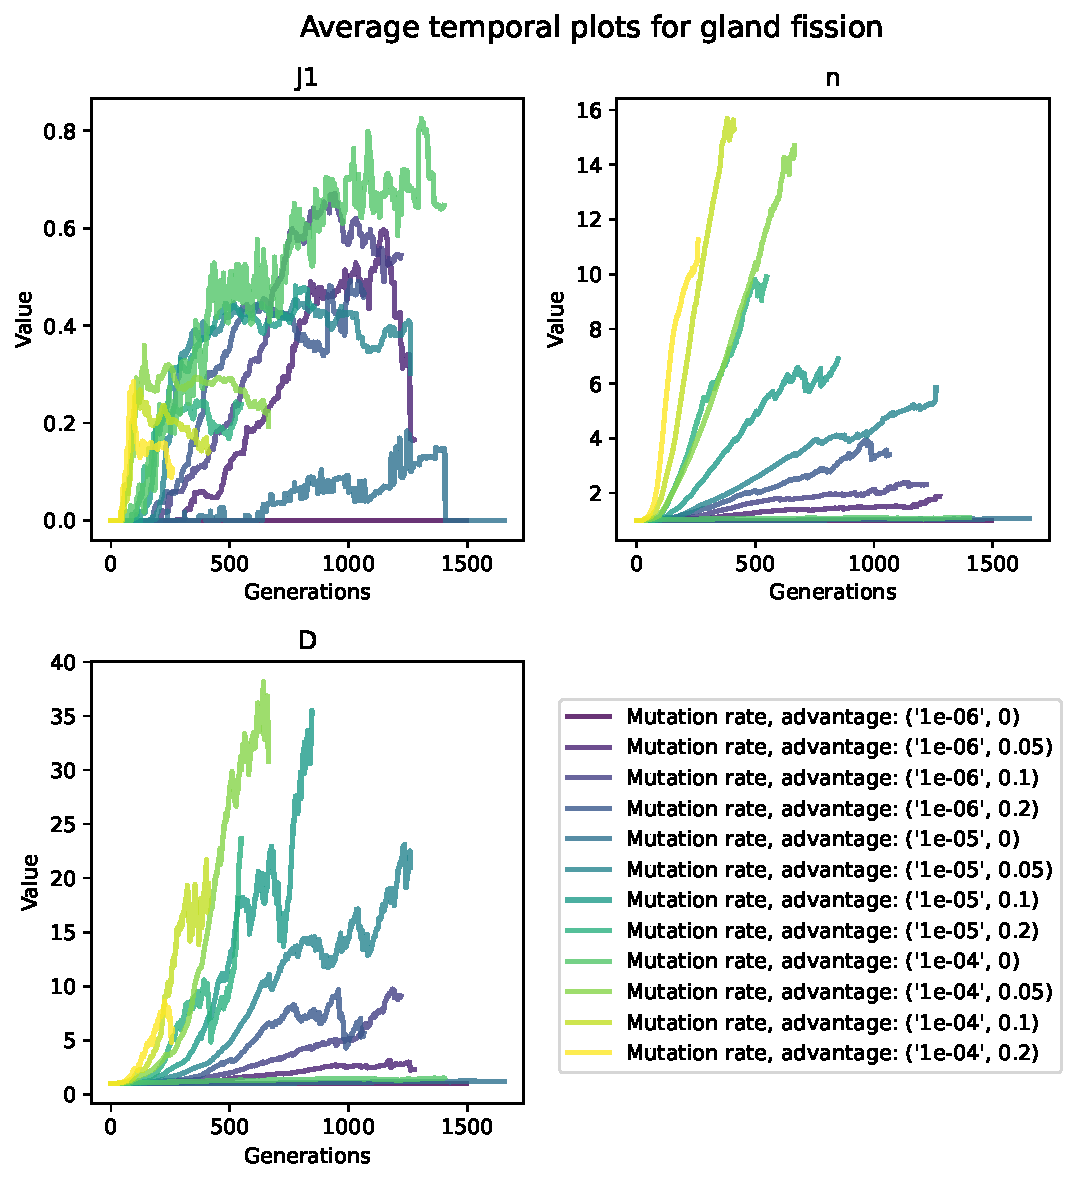
\includegraphics[width=\textwidth]{Chapter_3/figures/gland-temporal.pdf}
    \caption{Average trajectories of the three indices for different values of driver mutation rate and selective advantage for gland fission.}
    \label{fig:gland-temporal}
\end{figure}
\begin{figure}
    \centering
    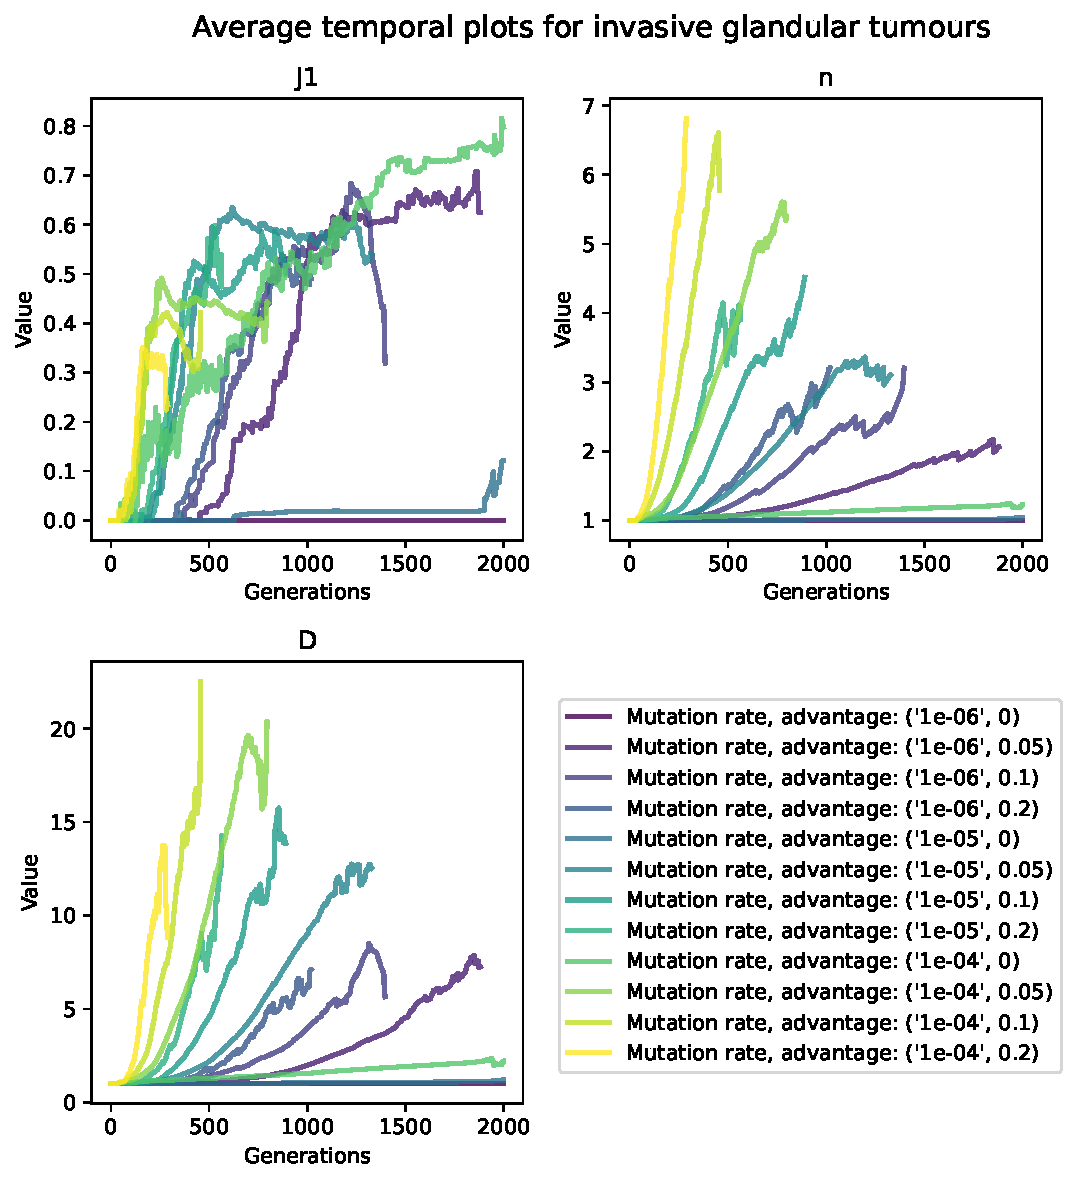
\includegraphics[width=\textwidth]{Chapter_3/figures/inv-gland-temporal.pdf}
    \caption{Average trajectories of the three indices for different values of driver mutation rate and selective advantage for invasive glandular tumours.}
    \label{fig:inv-gland-temporal}
\end{figure}
TO DO: add figures for index space, add figures to appendix, add expanded index set figures (both temporal and index space)
\begin{figure}
    \centering
    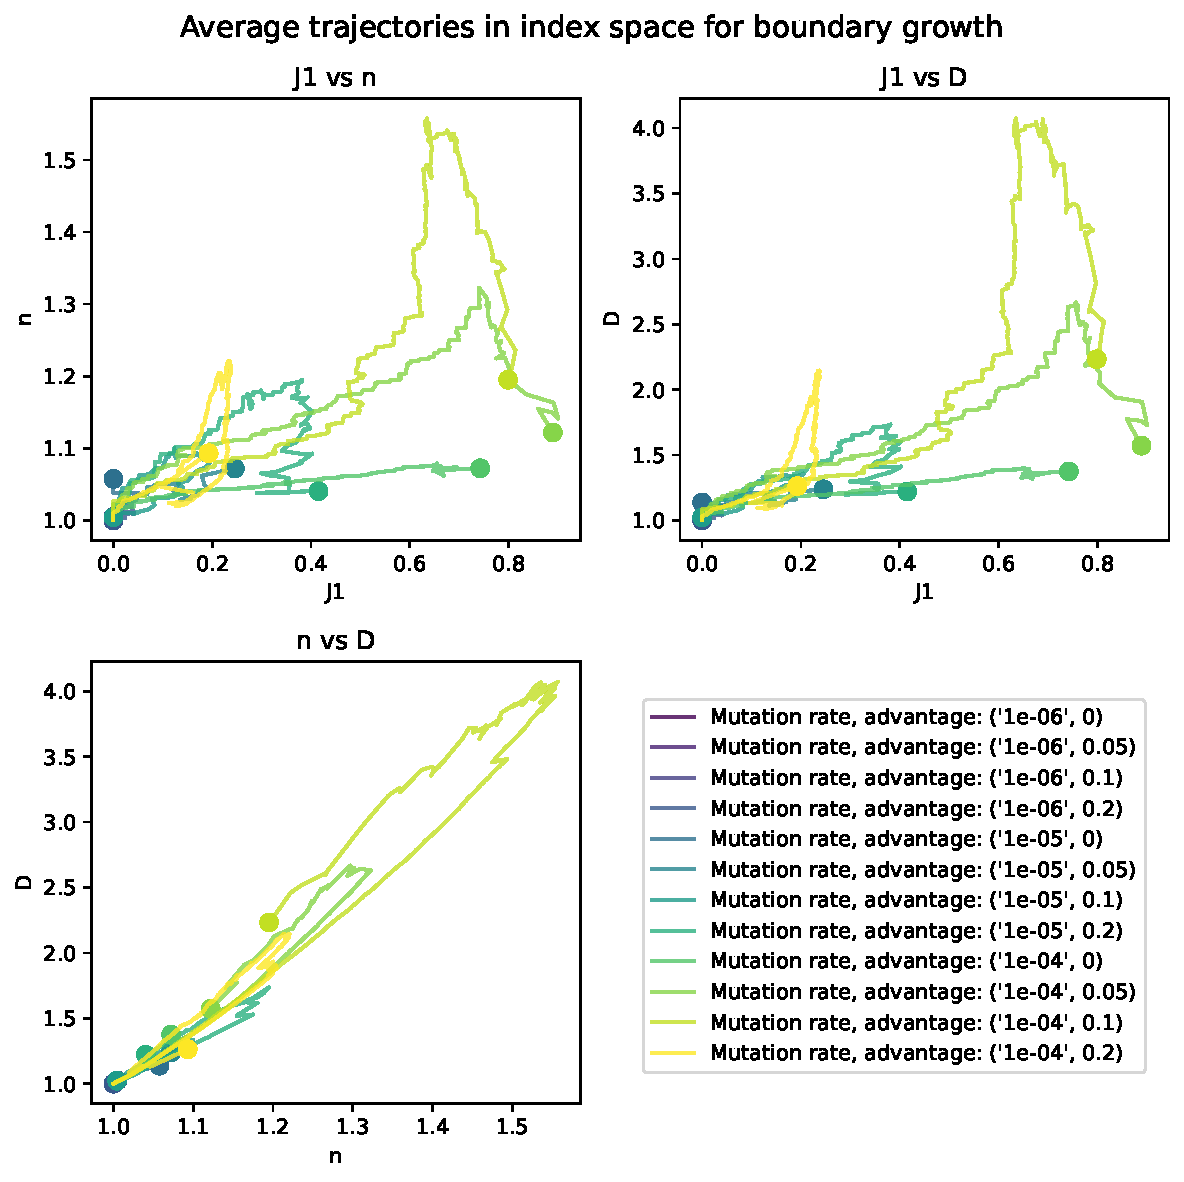
\includegraphics[width=\textwidth]{Chapter_3/figures/indspace-boundary.pdf}
    \caption{Average trajectories in index space for tumours progressing via boundary growth.}
    \label{fig:boundary-indspace}
\end{figure}
\begin{figure}
    \centering
    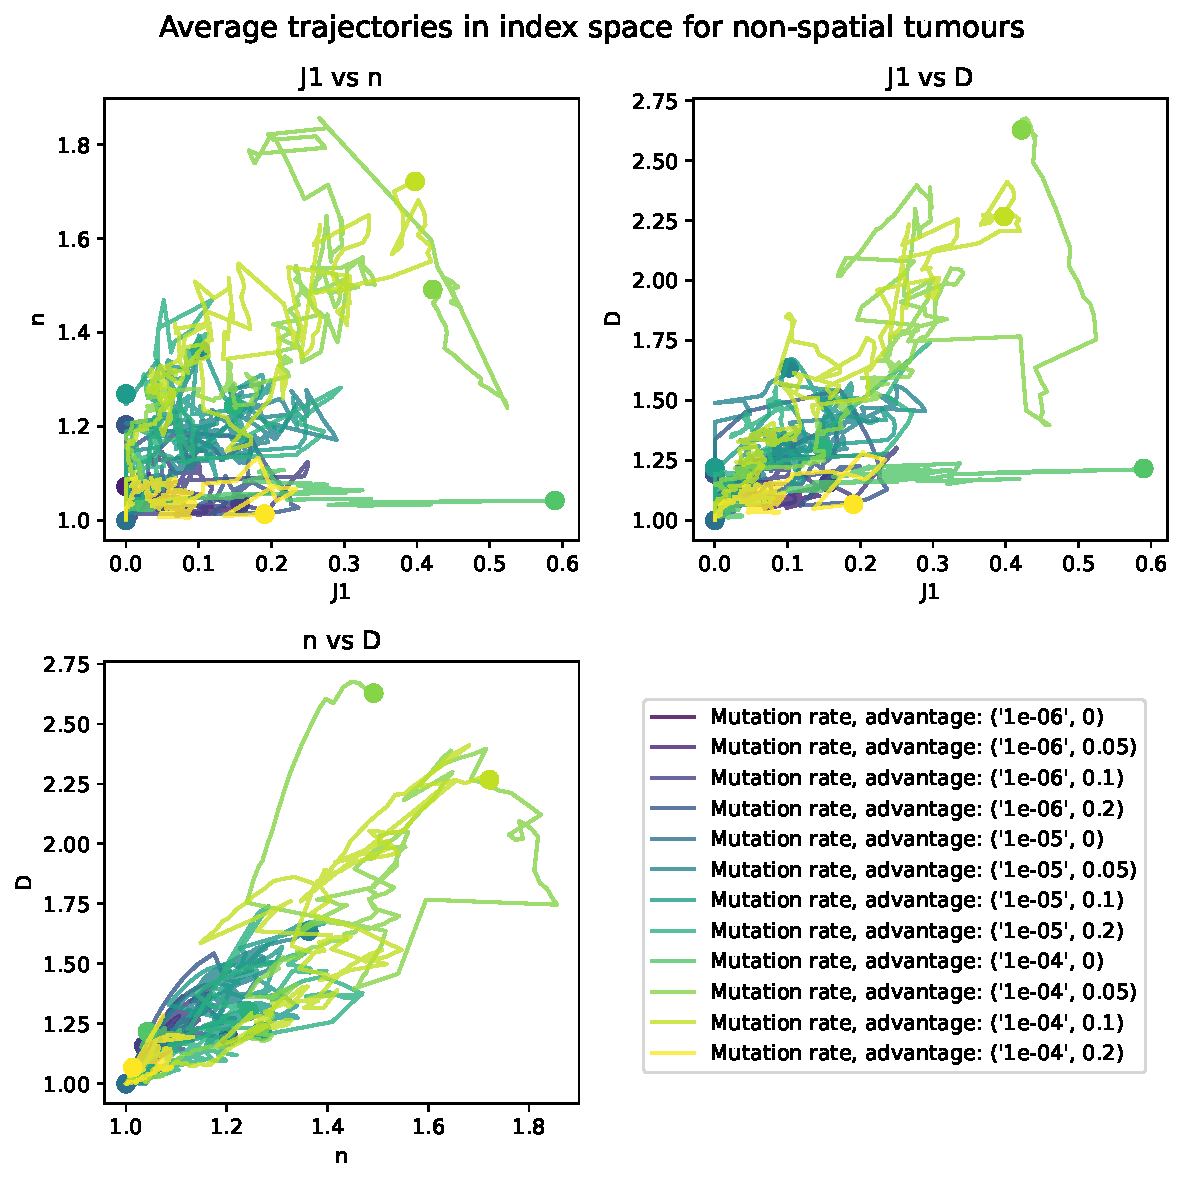
\includegraphics[width=\textwidth]{Chapter_3/figures/indspace-non-spatial.pdf}
    \caption{Average trajectories in index space for well-mixed cancer cell populations.}
    \label{fig:non-spatial-indspace}
\end{figure}
\begin{figure}
    \centering
    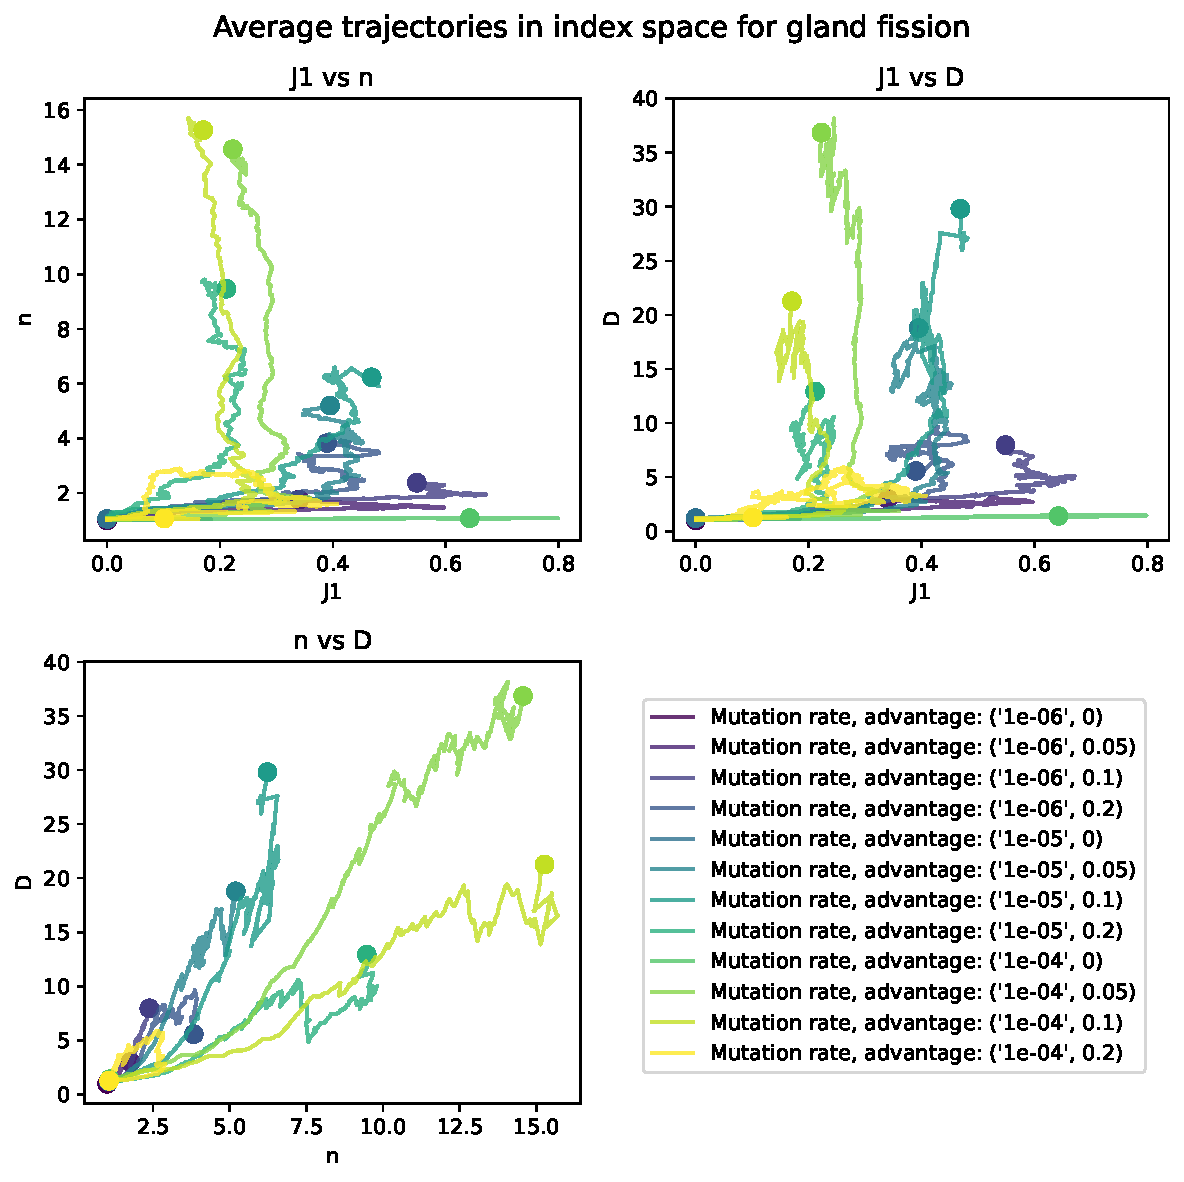
\includegraphics[width=\textwidth]{Chapter_3/figures/indspace-gland.pdf}
    \caption{Average trajectories in index space for tumours progressing via gland fission.}
    \label{fig:gland-indspace}
\end{figure}
\begin{figure}
    \centering
    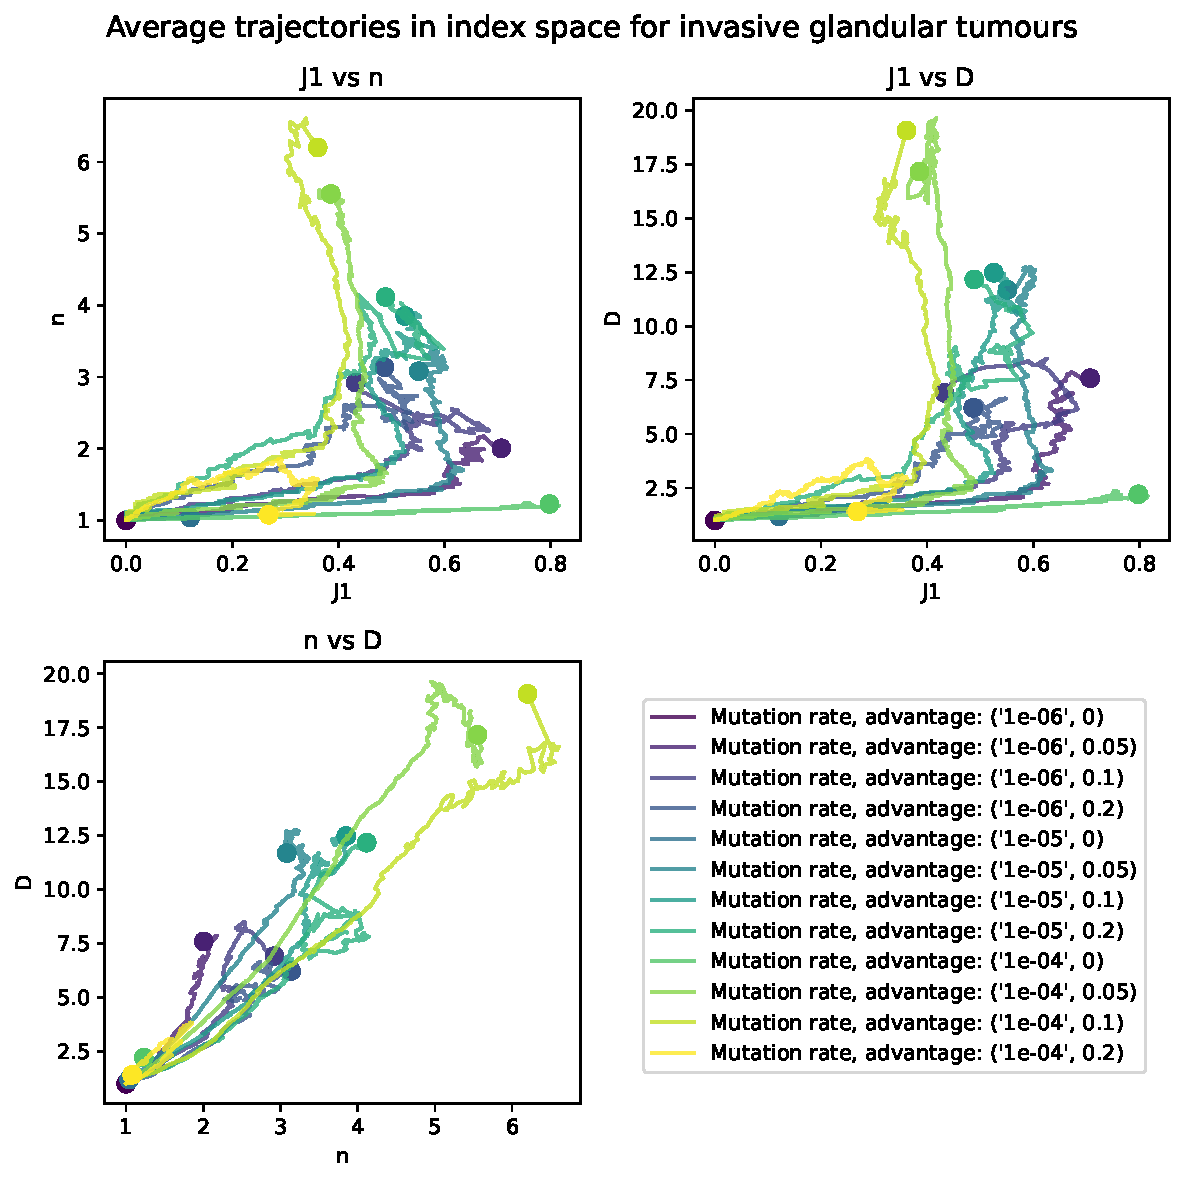
\includegraphics[width=\textwidth]{Chapter_3/figures/indspace-inv-gland.pdf}
    \caption{Average trajectories in index space for invasive glandular tumours.}
    \label{fig:inv-gland-indspace}
\end{figure}

% \subsection{Late-stage index-space location implies mode of evolution (?)}
% \begin{itemize}
%     \item focus on the overlaps between (average and overall) trajectories of different processes at later stages of tumour growth
%     \item consider differences between the base and expanded set of tree indices
%     \item based on outputs, come up with a summary statistic which could sort a tumour into different based on the end-of-growth state of the tree
% \end{itemize}

\section{Discussion}
\begin{itemize}
    \item clear differences between different tumour trajectories, but also decent amount of variance depending on parameters --- which ones are realistic? (need to be inferred from real data)
    \item what are the limitations of the approach? --- clear starting point is data availability, but also general inter-patient variation of tumour progression
    \item next steps --- further refining of the methods, sourcing and applying to more data (Kim's work in progress)
\end{itemize}

\chapter{Agent-based workflow for inferring evolutionary parameters from molecular data using approximate Bayesian computation}\label{demonchap}
In this chapter, I will go over the methods I have used and developed for work on data in chapter \ref{methchap}.

\section{Introduction}
\subsection{Spatial agent-based modelling}
\begin{itemize}
    \item go over a few relevant models in the field and how they compare to demon
    \item discuss the general assumptions and limitations of ABM
\end{itemize}


\subsection{Approximate Bayesian computation (ABC)}
\begin{itemize}
    \item high-level introduction of ABC
    \item papers in the field which have used some form of ABC
\end{itemize}

\section{Initial simulation workflows}
\begin{itemize}
    \item go over the old \texttt{demon} simulations with \texttt{demonmeth} R package analysis
    \item discuss why the approach worked
    \item point out the ways in which it didn't exactly work (i.e. impossible to get independent methylation and demethylation rates; output files sometimes too large to import into R and analyse efficiently; sometimes large files may not contain all the required data)
\end{itemize}

\section{Simulating fluctuating methylation arrays with \texttt{methdemon}}
\subsection{Overview}
\begin{itemize}
    \item go over the simulation's inner workings
    \item provide estimates of running efficiency and memory requirements
    \item discuss possible upgrades and their potential computational costs
\end{itemize}
\subsection{Examples}
Provide example outputs (and their visualisations), parameter tables and a citation/link to the github repo.

\section{Fluctuating methylation arrays through the lens of ABC}
\subsection{Overview}
\begin{itemize}
    \item go over the \texttt{pyabc} package briefly (cite)
    \item explain the ABC workflow
    \item discuss computational costs and efficiency
    \item discuss whether this is the best approach (can we write down a likelihood for the problem?)
\end{itemize}
\subsection{Examples}
Provide example applications of the workflow to \texttt{methdemon} outputs - fit smaller simulations to a big one for example.

\chapter{Modelling colorectal cancer methylation data with \texttt{methdemon}}
\label{chapter:methylation}
% \large\textbf{OUTLINE}
% \begin{itemize}
%     \item Introduction - methylation modelling literature, data collection
%     \item Results; sections: methdemon recapitulates FMC patterns in crc,
%         evolutionary regimes which explain the data within methdemon,
%         phylogenetic tree analysis
%     \item Discussion
% \end{itemize}

\section{Introduction}
A mathematical model is only as good as its ability to describe its system of
interest. Therefore, in this chapter, I will test how well the
\texttt{methdemon} model describes methylation data sampled from colorectal
cancer (CRC). CRC is the third most common cancer worldwide, with over $40000$
new cases diagnosed in the UK each year on average
\cite{cancer_research_uk_bowel_2021}. The disease is characterised by the
accumulation of genetic and epigenetic mutations in colonic cells
\cite{fleming_colorectal_2012}. The most common type of CRC is adenocarcinoma,
which arises from the epithelial cells lining the colon, covering the majority
of cases. The tumour forms hierarchical cell structures similar to those of
normal tissue, organising into crypt-like glands
\cite{ponz_de_leon_pathology_2001}. The tumour spreads by the process of gland
fission \cite{preston_bottom-up_nodate}, which is similar to the branching
processes seen in normal crypts \cite{almet_multicellular_2018}.

\section{Data collection}
The data used in this study were provided by Dr Darryl Shibata from the Keck
School of Medicine at the University of Southern California. The data consist
of DNA methylation arrays sequenced from multiple glands within colorectal
tumours post-surgery. All samples are anonymised. The arrays were obtained from
bulk samples of tumour glands, which means that the data are nominally not
single-cell resolved. Each tumour sample consists of $8$ glands, with each
gland's array containing some $850000$ CpG sites. The arrays were obtained
using the Illumina Infinium MethylationEPIC BeadChip array. The data were
pre-processed by Dr Shibata to remove low-quality samples and normalise the
arrays. The sample purity was high, with the vast majority of cells in the
samples being tumour cells.

\section{Results}
\subsection{Identification of fCpG loci in colorectal cancer}
The first step in the analysis was to identify the fCpG loci in the data. As
multiple samples come from the same tumour, a larger cohort of samples is
needed to reliably identify fCpG loci using the methods described by
\cite{gabbutt_evolutionary_2023}, i.e. isolating a set of CpG loci which are
the least informative about the methylation state across the cohort. Dr Gabbutt
ran the analysis on colorectal cancer data from the Cancer Genome Atlas (TCGA)
and identified $1258$ fCpG loci. For comparison, I ran a similar analysis only
on the data provided by Dr Shibata and identified a set of some $950$ loci. Of
these, only $120$ were common to both sets. The discrepancy is likely due to
the small sample size of the data provided by Dr Shibata. The fCpG loci
identified in one of the samples are shown in figure \ref{fig:fCpG_loci_M},
with additional figures in appendix \ref{appendix:fCpG_loci}.

\begin{figure}[h]
    \centering
    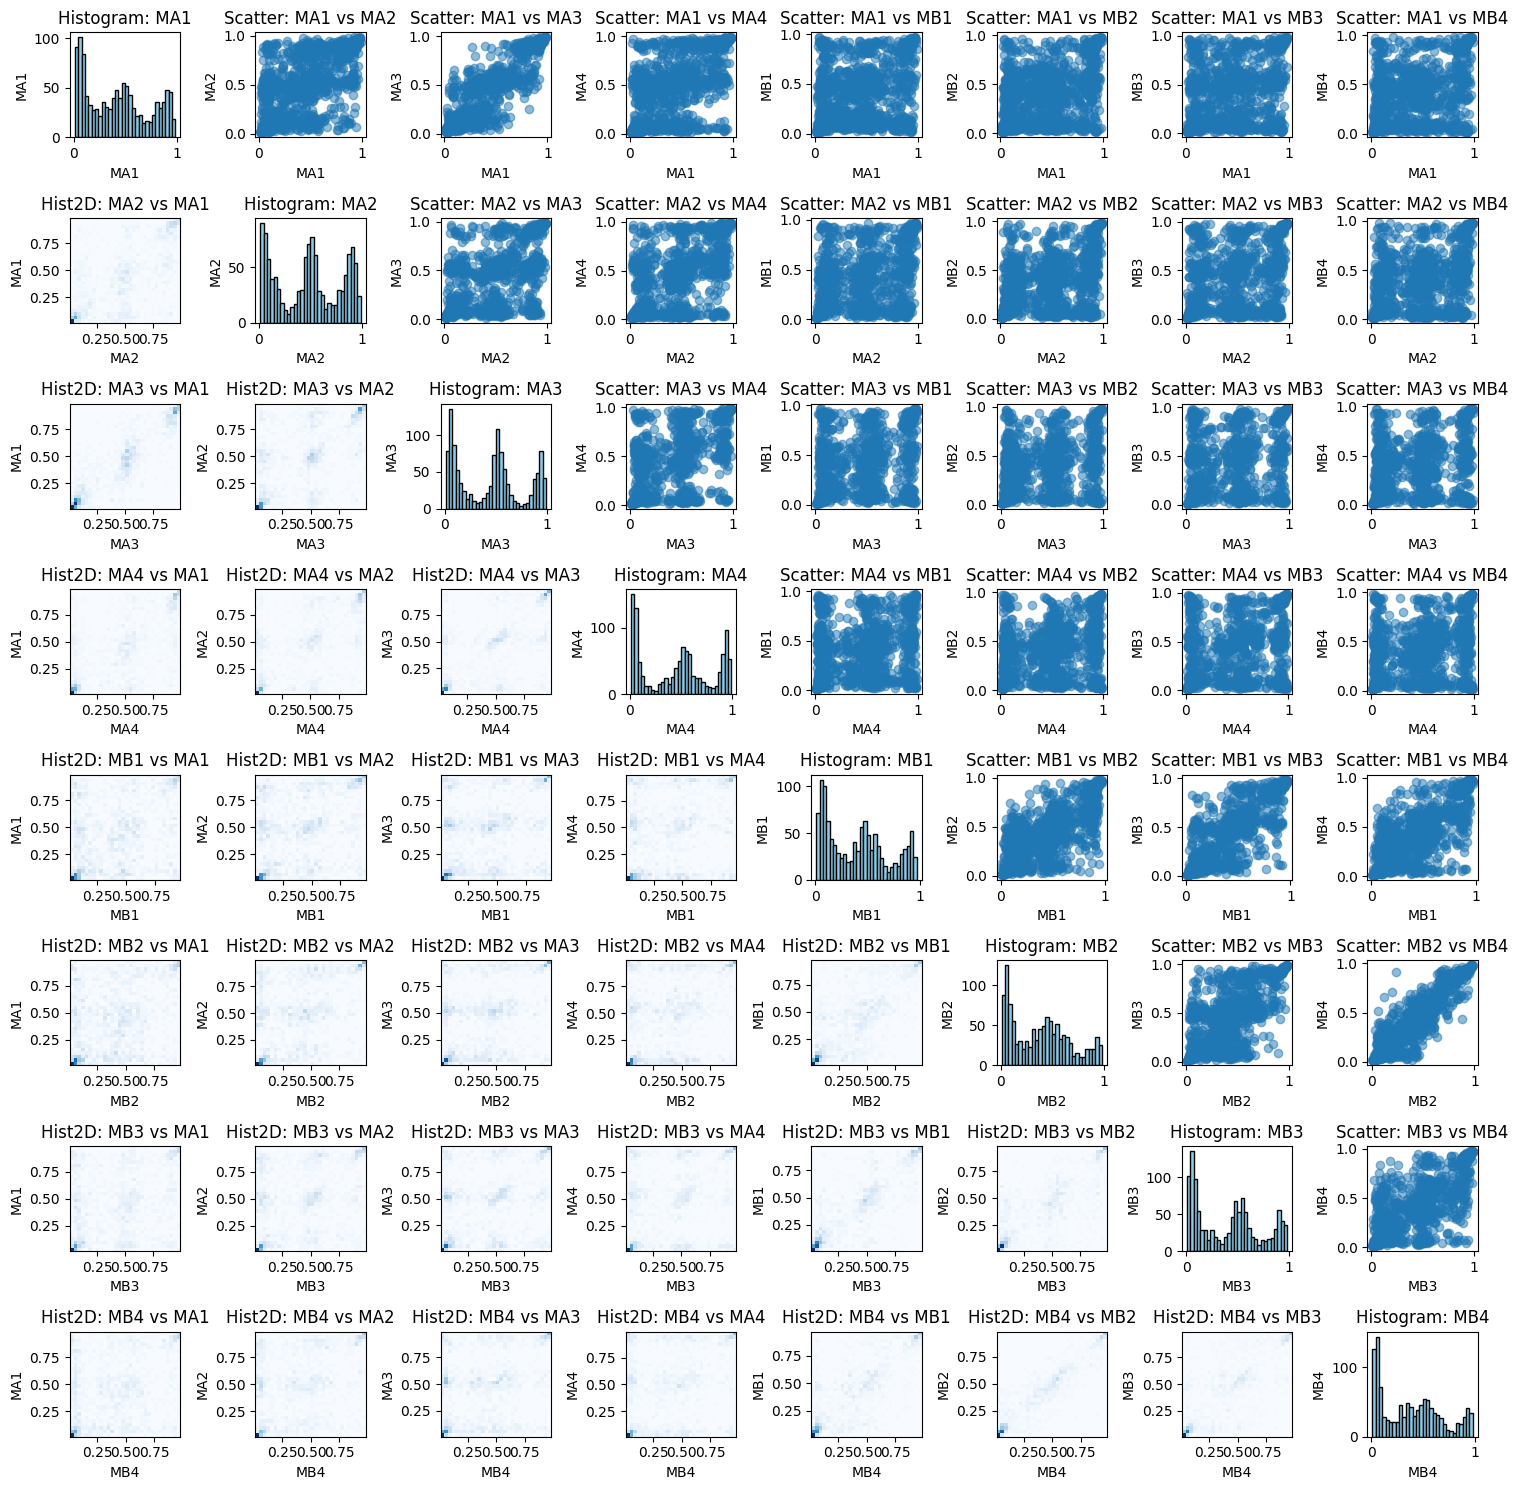
\includegraphics[width=\textwidth]{Chapter_5/figures/fCpG_loci_M.png}
    \caption{Glands from the same side (A, B) of the tumour have more similar
    fCpG arrays than glands from different sides. \textbf{diagonal} ---
    histograms of fCpG arrays for each gland; \textbf{above diagonal} ---
    scatter plots of correlations between glands; \textbf{below diagonal} ---
    $2$D histograms of the above-diagonal plots, showing the density of points.}
    \label{fig:fCpG_loci_M}
\end{figure}

A notable feature of the data is that some samples show a clear bias towards
either hyper- or hypomethylation. This was also the case for fCpG arrays
filtered using only the samples provided by Dr Shibata. This suggests that the
progenitor cell's methylation state is not necessarily random, but could be
affected by internal or external factors. Furthermore, I developed the model
under the assumption that methylation and demethylation rates are constant and
equal across all cells and fCpG loci. While this may be reasonable on average,
there might be mutations which affect these rates, leading to the observed
distributions of fCpG loci states.

\subsection{Spatial proximity predicts similarity between fCpG arrays}
With the assumed hierarchical structure of the tumour in mind, it should make
sense intuitively that glands which are spatially close to each other likely
diverged more recently than glands which are further apart. As a result, they
have spent less time evolving independently and should have more similar fCpG
arrays. To test this hypothesis, I calculated the inter-gland distance matrix
for each tumour sample. The resulting matrices show a clear correlation between
side and distance values. The distance matrix for one of the samples is shown
in figure \ref{fig:gland_dist_M} for tumour M, and in appendix
\ref{appendix:gland_distances} for the other samples.

\begin{figure}[h]
    \centering
    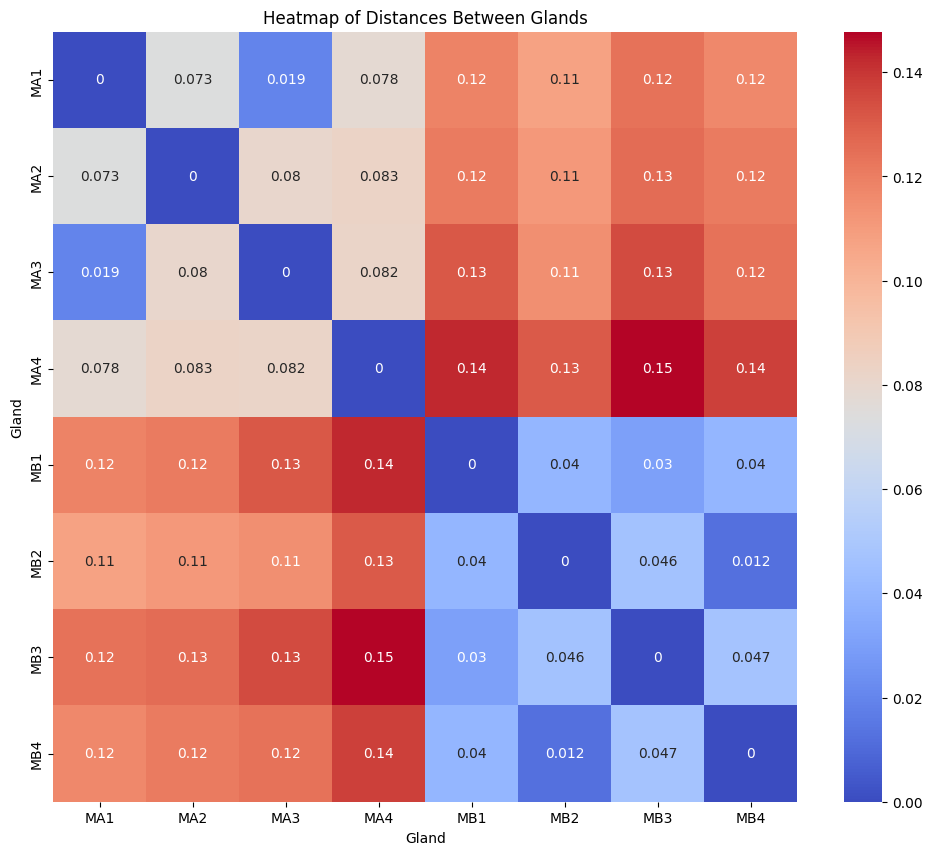
\includegraphics[width=\textwidth]{Chapter_5/figures/gland_dist_M.png}
    \caption{The inter-gland distance matrix for tumour M shows that spatial
    proximity is corelated to similarity between fCpG arrays.}
    \label{fig:gland_dist_M}
\end{figure}

\subsection{Development of the \texttt{methdemon} model}
The \texttt{methdemon} model was developed for the purpose of simulating the
data provided by Dr Shibata. The model's assumptions are based on the general
understanding of colorectal cancer evolution and, translated into the language
of an agent-based model, are as follows:

\begin{enumerate}[(i)]
    \item \textbf{A single cell forms the first gland and initiates tumour
        growth.} This assumption skips over the process of tumorigenesis,
        during which a cell accumulates mutations and becomes malignant
        \cite{tariq_colorectal_2016}. This is a simplification to be sure, but
        a reasonable one, given that the focus of this work is on the
        evolutionary dynamics of the tumour rather than its initiation.
    \item \textbf{The rate of driver mutations is Poisson distributed and
        identical for all cells.} This assumption is consistent with most
        models of tumour evolution \cite{metzcar_review_2019,
        niida_modeling_2021}.
    \item \textbf{The cell population within a gland grows exponentially and is
        well-mixed.} While not necessarily consistent with the biology of a
        solid tumour, this assumption allows for more efficiency in the
        simulation as opposed to a multi-level spatial model. Further, as the
        data discussed in chapter \ref{chapter:methylation} is obtained from
        bulk samples of tumour glands, this assumption is not unreasonable.
        \label{item:well_mixed}
    \item \textbf{Once a gland reaches a certain size, which we call the
        carrying capacity, the population undergoes steady-state turnover
        according to the Moran process.}
    \item \textbf{At carrying capacity, a gland has a certain probability of
        undergoing fission, which splits the gland's population randomly into
        two.} As a consequence of assumption (\ref{item:well_mixed}), fissions
        do not take into account a gland's spatial organisation.
    \item \textbf{Gland fission occurs as a neutral spatial branching process.}
        The previous two assumptions and this one together form the basis of
        the model's spatial dynamics. While there are other mechanisms of
        colorectal adenocarcinoma progression, gland fission is the principal
        way in which the tumour grows \cite{preston_bottom-up_nodate}. The
        assumption of neutrality in the spatial branching process is consistent
        with the findings of \cite{sottoriva_big_2015}. Additionally, this
        assumption is based on the fact that the data used in this study only
        contains information about whether a gland was sample from side A or B,
        without any further spatial information other than the approximate size
        of the full tumour.
\end{enumerate}

\subsection{Higher deme carrying capacity requires stronger selection to
recapitulate the data}
To begin the analysis of cancer data using the \texttt{methdemon} model, I tested the
ranges of parameters based on the assumption that each cancer cell has infinite
proliferative potential. This would mean setting the carrying capacity of a gland
to about $10000$ cells, which is consistent with the size of the glands in the
literature \cite{sottoriva_big_2015} and our data. Due to the glandular
structure of the tumour, this is an effectively neutral model, as selection
acts within glands but not between them, leading to progressive diversification
of the population, as discussed in chapter \ref{chapter:trajectories} and
\cite{noble_spatial_2022}.\par

\begin{figure}[h]
    \centering
    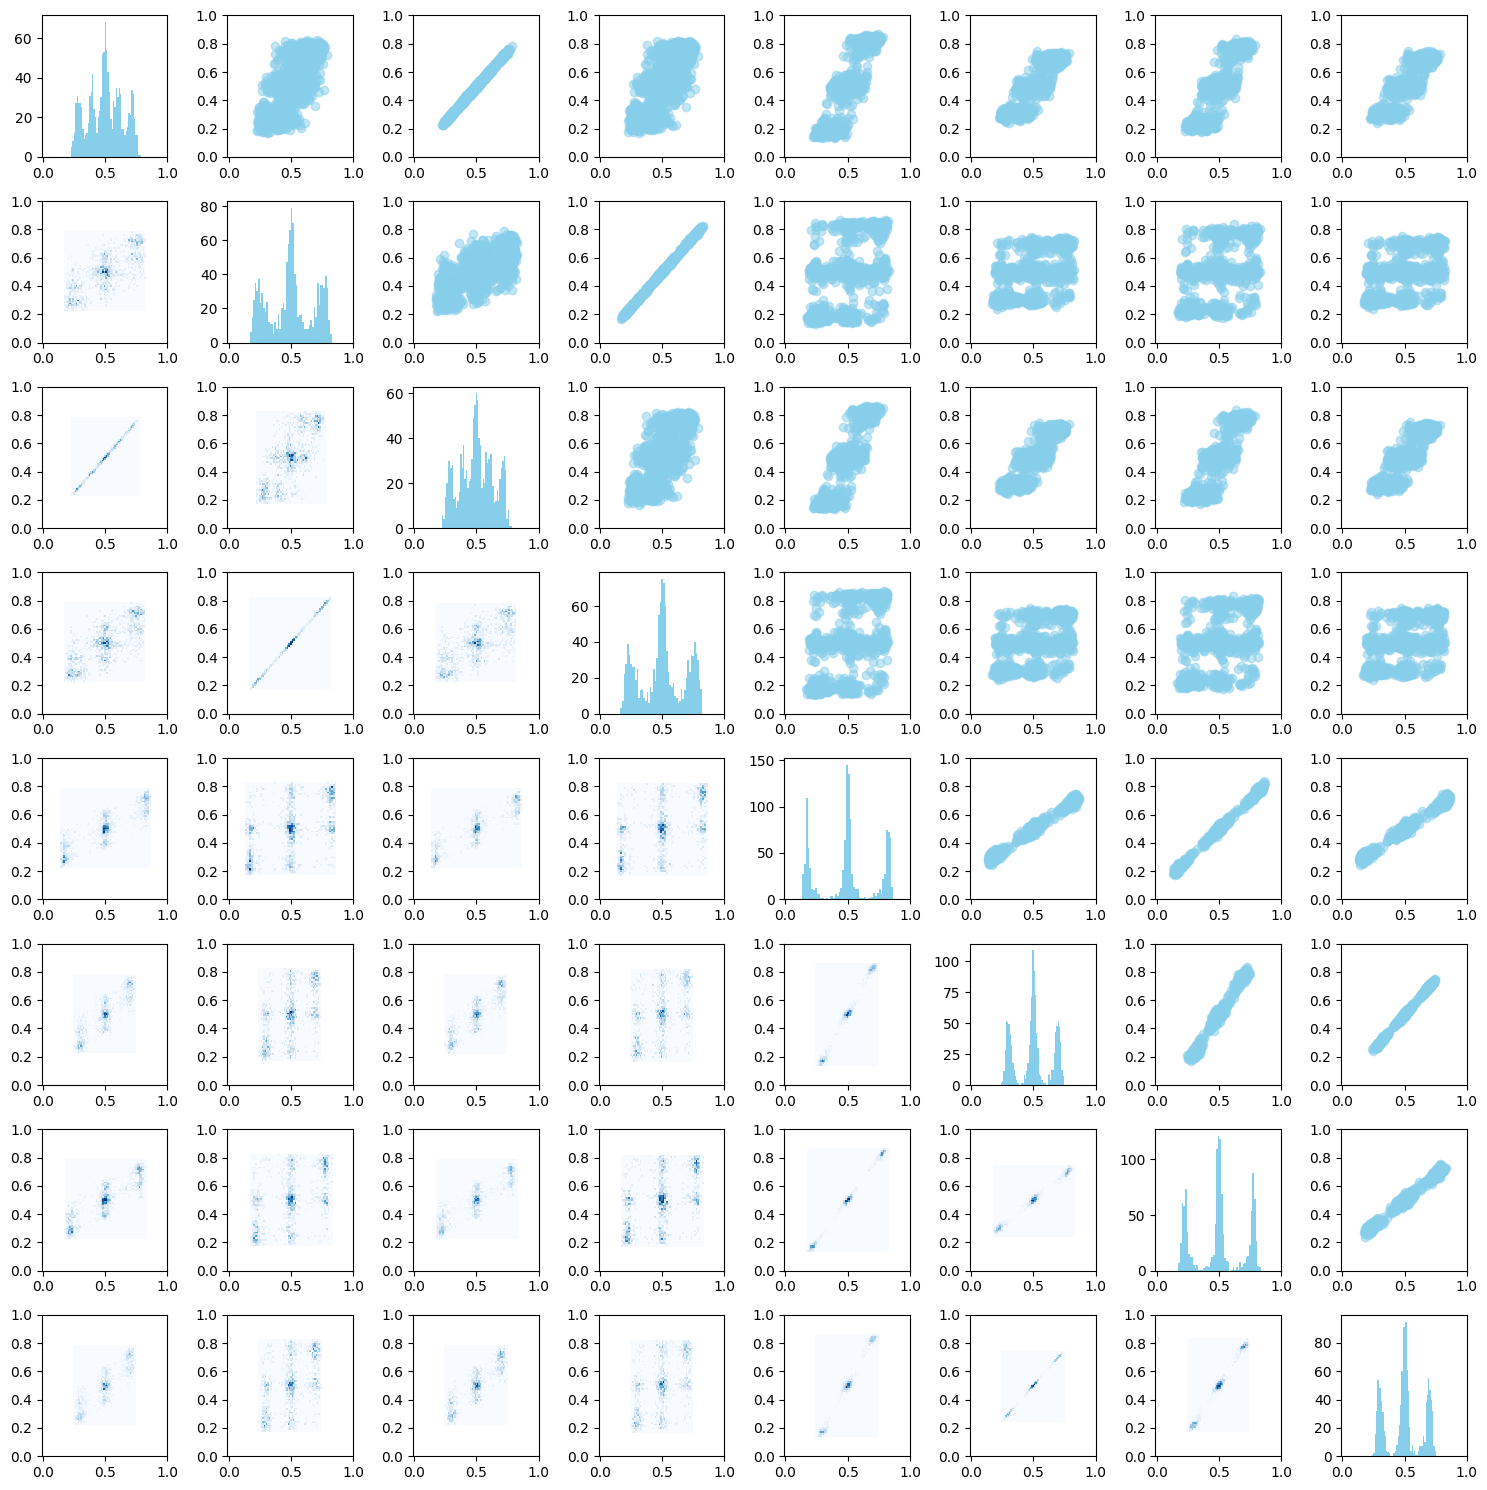
\includegraphics[width=\textwidth]{Chapter_5/figures/10000plot.png}
    \caption{}
    \label{fig:methdemon_weak_selection}
\end{figure}

\begin{figure}[h]
    \centering
    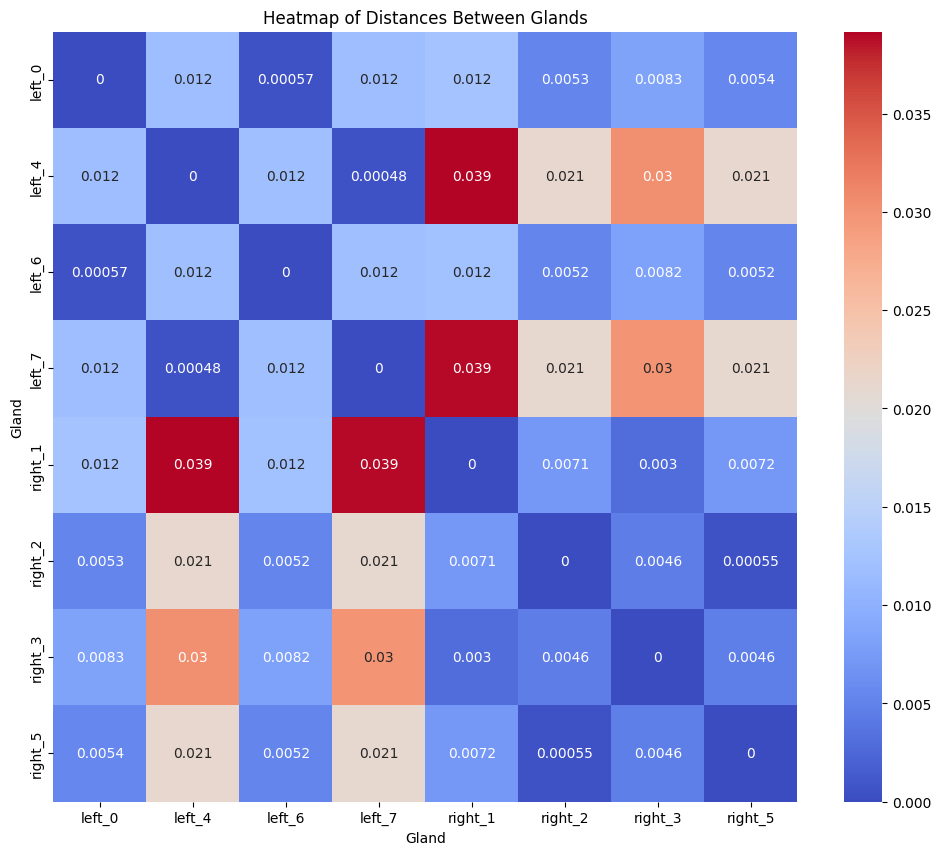
\includegraphics[width=\textwidth]{Chapter_5/figures/10000dist.png}
    \caption{Inter-gland distances for the output fCpG arrays from the
    \texttt{methdemon} model with weak selection.}
    \label{fig:methdemon_weak_dist}
\end{figure}

As a first test, I ran the model with weak selection, $s=0.1$. The resulting
outputs are shown in figures \ref{fig:methdemon_weak_selection} and
\ref{fig:methdemon_weak_dist}. There are a few notable features about the
output fCpG arrays and the distance matrix. The most obvious is that the peaks
associated with homozygous methylation and demethylation states have moved
towards the middle. This is to be expected, as we are treating all $10000$ cells
in a deme as being able to divide ad infinitum, leading to a lot of stochastic
noise. This is a consequence of the time spent in turnover, and is adjusted by
increasing the fission rate. However, the distance matrix shows that the glands
are still very similar to each other, especially when compared to the data. This
is likely due to the fact that there is only a small probability of a partial or
full sweep of a lineage within a gland. The similarity is a consequence of the
large deme carrying capacity, which allows for a lot of stochastic noise to
accumulate over time but lowers the probability of fixation in the weak
selection regime. Increasing the selection coefficient to $s=0.3$ leads to more
divergence between the glands, since emerging lineages are more likely to fully
or partially sweep the gland's population and establish more distinct fCpG
arrays between glands. However, as discussed in chapter \ref{chapter:methdemon},
strong selection can quickly become problematic in an ABM like this due to the
accumulation of advantageous drivers. An example of strong selection at deme
size $10000$ is in appendix \ref{appendix:inference}. \par
Considering that the number of stem cells in a normal crypt is on the order of
$10$ \cite{gehart_tales_2019, gabbutt_fluctuating_2022}, with the total number
of cells in a crypt being on the order of $1000$, I next tested the model with
a deme carrying capacity of $100$ i.e. about $1\%$ of the total cell population
in the gland. The currently available data supports this percentage as a
reasonable estimate of the proportion of cancer stem cells (CSCs) in colorectal
cancer \cite{obrien_human_2007, munro_cancer_2018}. In this case, the model's
outputs are as expected, with the fCpG arrays diverging over time even with no
or weak selection. Examples are shown in figures
\ref{fig:methdemon_weak_selection_small} and
\ref{fig:methdemon_weak_dist_small}.

\begin{figure}[h]
    \centering
    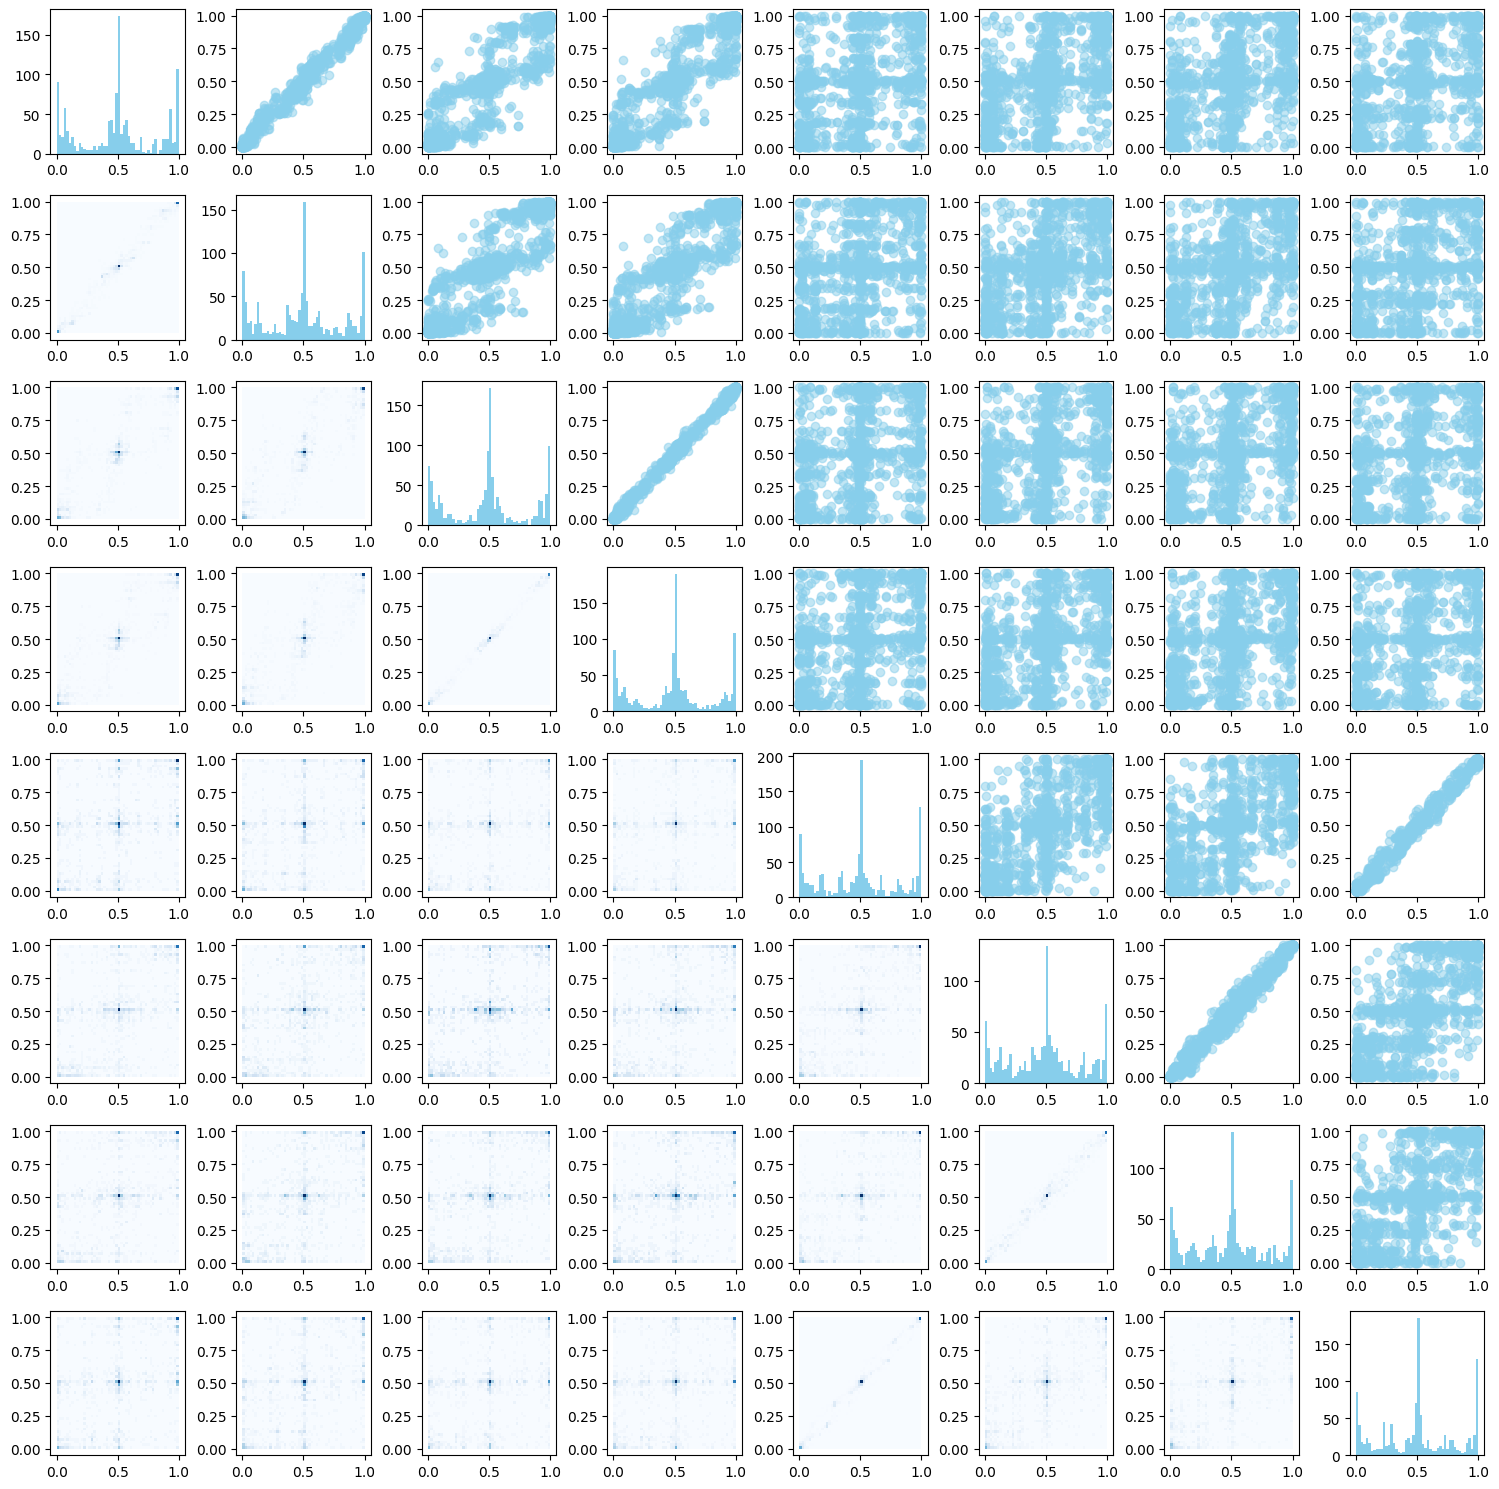
\includegraphics[width=\textwidth]{Chapter_5/figures/100plot.png}
    \caption{Output fCpG arrays from the \texttt{methdemon} model with weak
    selection and deme carrying capacity $100$ reflect the data better than
    larger deme carrying capacity.}
    \label{fig:methdemon_weak_selection_small}
\end{figure}

\begin{figure}[h]
    \centering
    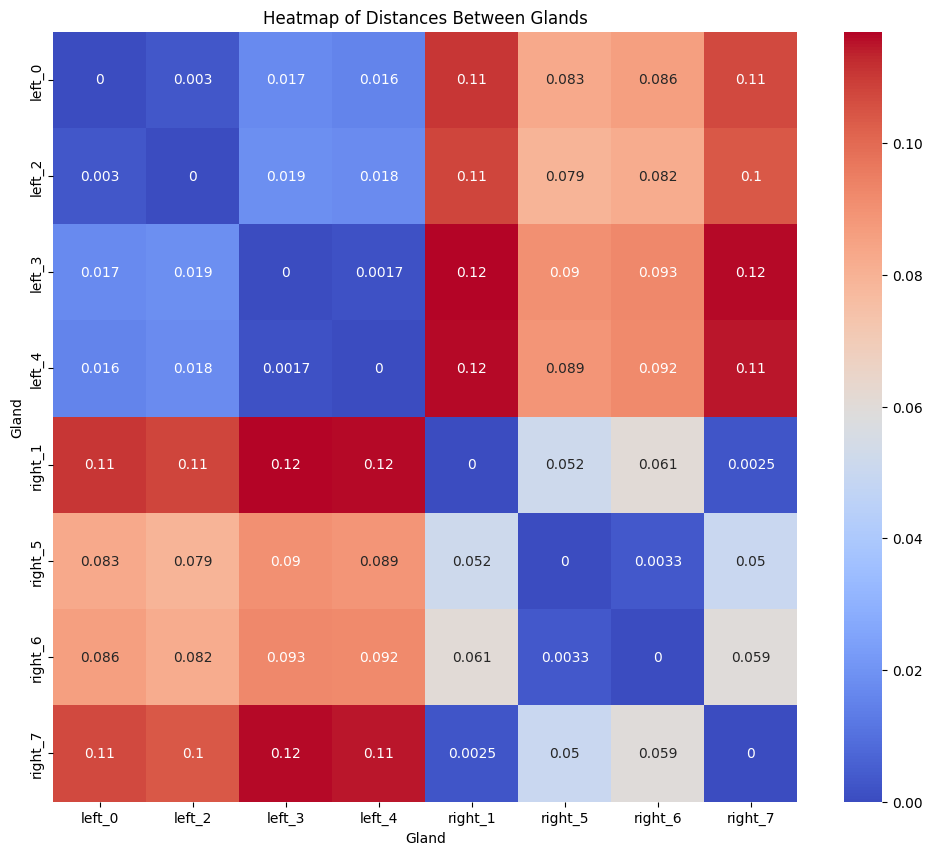
\includegraphics[width=\textwidth]{Chapter_5/figures/100dist.png}
    \caption{Inter-gland distance matrix corresponding to the run from figure
    \ref{fig:methdemon_weak_selection_small}.}
    \label{fig:methdemon_weak_dist_small}
\end{figure}
\clearpage

\subsection{Parameter inference from colorectal cancer data}
\subsubsection{Regular model}
Having established \texttt{methdemon}'s ability to output data which resembles
observations, I next attempted to fit the model to the colorectal cancer data.
For this, I used the ABC workflow described in chapter \ref{chapter:methdemon}.
Considering the results of the previous section, I set the deme carrying
capacity to $100$ for all inference runs. I made this choice as there is no
evidence to suggest different numbers of stem cells across tumours or even
glands within a tumour. Furthermore, having the deme carrying capacity as a free
parameter would slow down the inference process significantly.
In the first instance, I ran the inference with parameter ranges given in table
\ref{tab:inf_ranges}. The results of the inference are shown in figure
\ref{fig:inference_1}, with more details in appendix \ref{appendix:inference}.

\begin{table}[ht]
\centering
\begin{tabular}{|l|l|l|}
\hline
Parameter & Prior \\
\hline
methylation rate & $U(0, 0.1)$ \\
demethylation rate & $U(0, 0.1)$ \\
fission rate & $U(10^{-4}, 10^{-2})$ \\
driver mutation rate & $U(0, 10^{-2})$ \\
selective advantage & $U(0, 0.2)$ \\
\hline
\end{tabular}
\caption{Parameter priors for the first inference run.}
\label{tab:inf_ranges}
\end{table}

The first inference run did produce some results, but the posterior
distributions of some parameters remained broad. There are a few possible
reasons for this. Firstly, I intentianally used overly broad priors to see how
well the ABC workflow would delineate the parameter space. This choice makes the
inference process more dificult, as the prior distributions are not informative
and the parameter space is large. However, it allows for future runs with more
informative priors. The second reason may just be that the model is not able to
recover all of the parameters in its current form. Selective advantage and
driver mutation rate in particular seem to be difficult to infer for the model.
This could be due to the signature of selection being too weak in the model or
data (or both). It could also be down to the distance functions in the ABC
rejection step not being able to capture the differences between the arrays
well enough. Either way, the results prompted further testing with the important
change of log-transforming the parameters. This change allows for more efficient
exploration of the parameter space, as parameters are sampled on the same scale
and steps between generations will cover more of the space.

\begin{figure}[h]
    \centering
    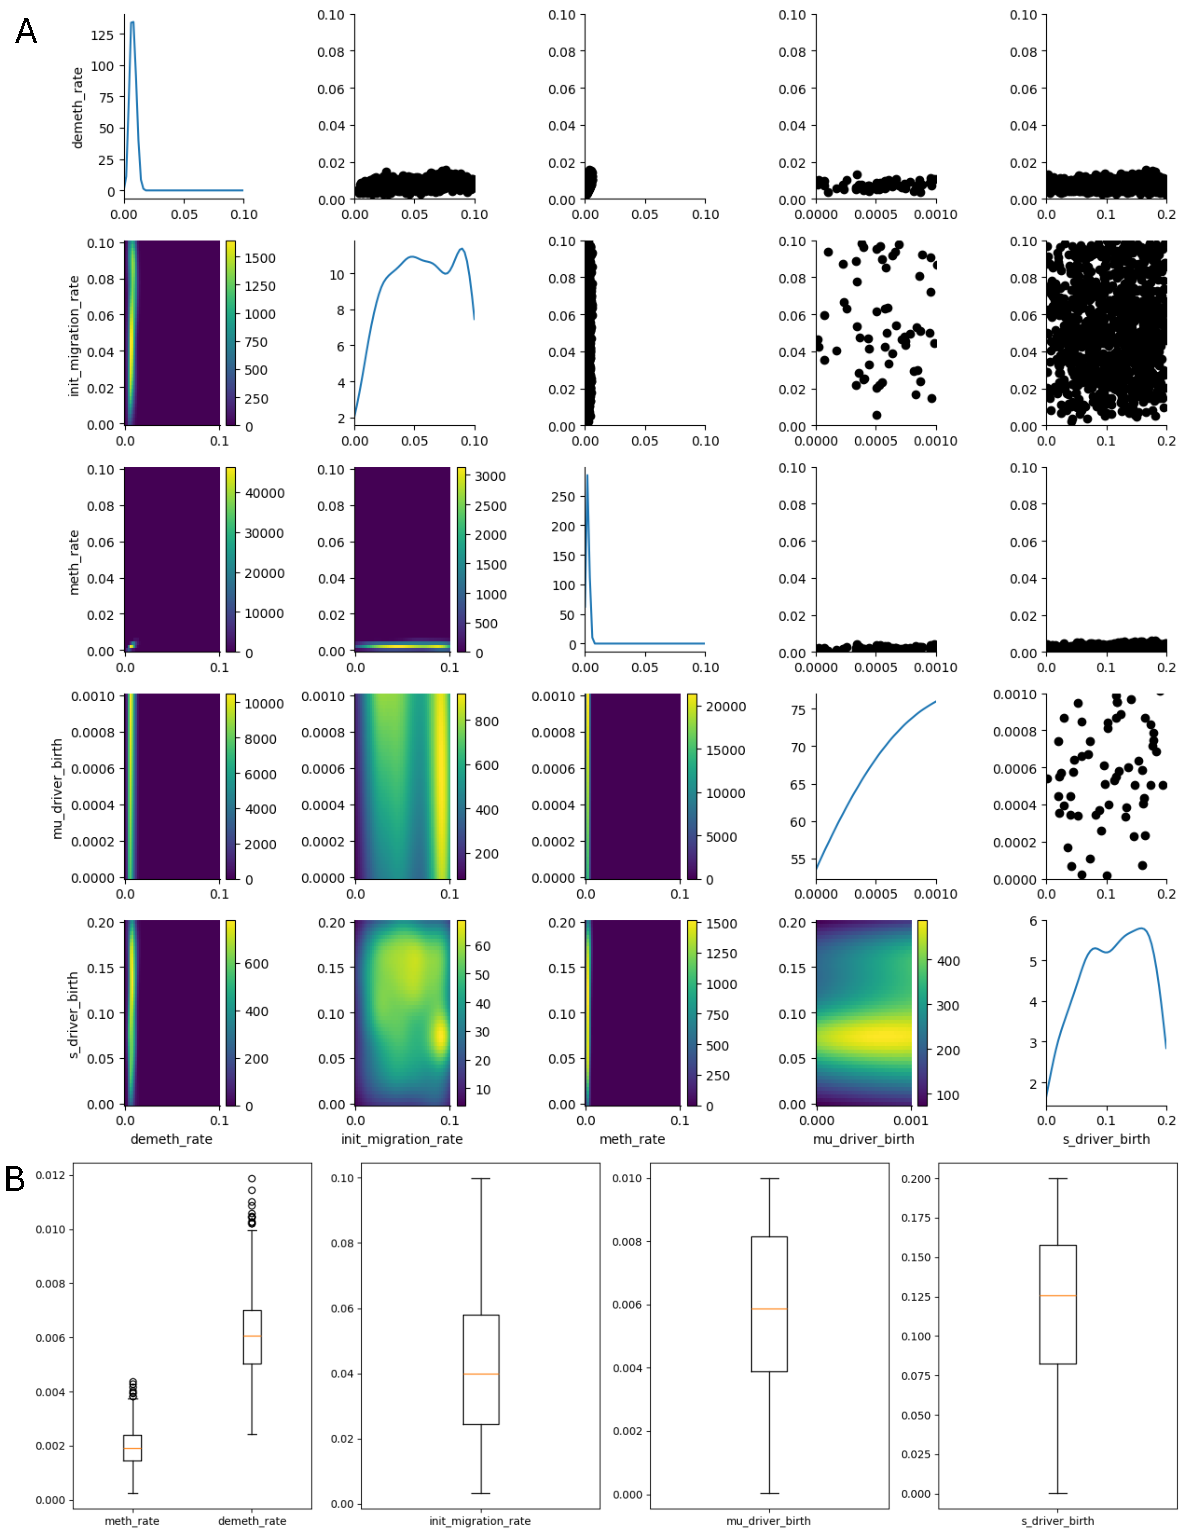
\includegraphics[width=\textwidth]{Chapter_5/figures/inference_raw/inference_1.pdf}
    \caption{Using absolute parameter values in the inference process leads to
    less efficient inference. \textbf{A} --- posterior distributions of fCpG
    fluctuation rates have narrowed down rapidly, but other parameters'
    posteriors remain broad. \textbf{B} --- box plots of the posteriors show
    that the model is not able to resolve the effects of selection from the
    data, and leaves a lot of uncertainty in the fission rates.}
    \label{fig:inference_1}
\end{figure}
\clearpage

\subsubsection{Log-transformed model}
The second inference run was done with similar parameter ranges as the first.
The log-transformed parameter ranges are give in table \ref{tab:inf_ranges_log}
and the results of the inference are shown in figure \ref{fig:inference_2}, with
more details in appendix \ref{appendix:inference}. All log transformations were
done with base $10$.

\begin{table}[ht]
\centering
\begin{tabular}{|l|l|l|}
\hline
Parameter & Prior \\
\hline
log methylation rate & $U(-4, -2)$ \\
log demethylation rate & $U(-4, -2)$\\
log fission rate & $U(-3.3, -1)$\\
log driver mutation rate & $U(-5, -2)$\\
selective advantage & $U(0, 0.2)$\\
\hline
\end{tabular}
\caption{Log-transformed priors for the second inference run.}
\label{tab:inf_ranges_log}
\end{table}

The results of the second inference run are more promising than the first, with
the fission rate posterior distribution being considerably narrower. However,
selection and driver mutation rate are still difficult to narrow down. This
further supports the idea that the model is not able to detect weak selection
at the gland level.

\begin{figure}[h]
    \centering
    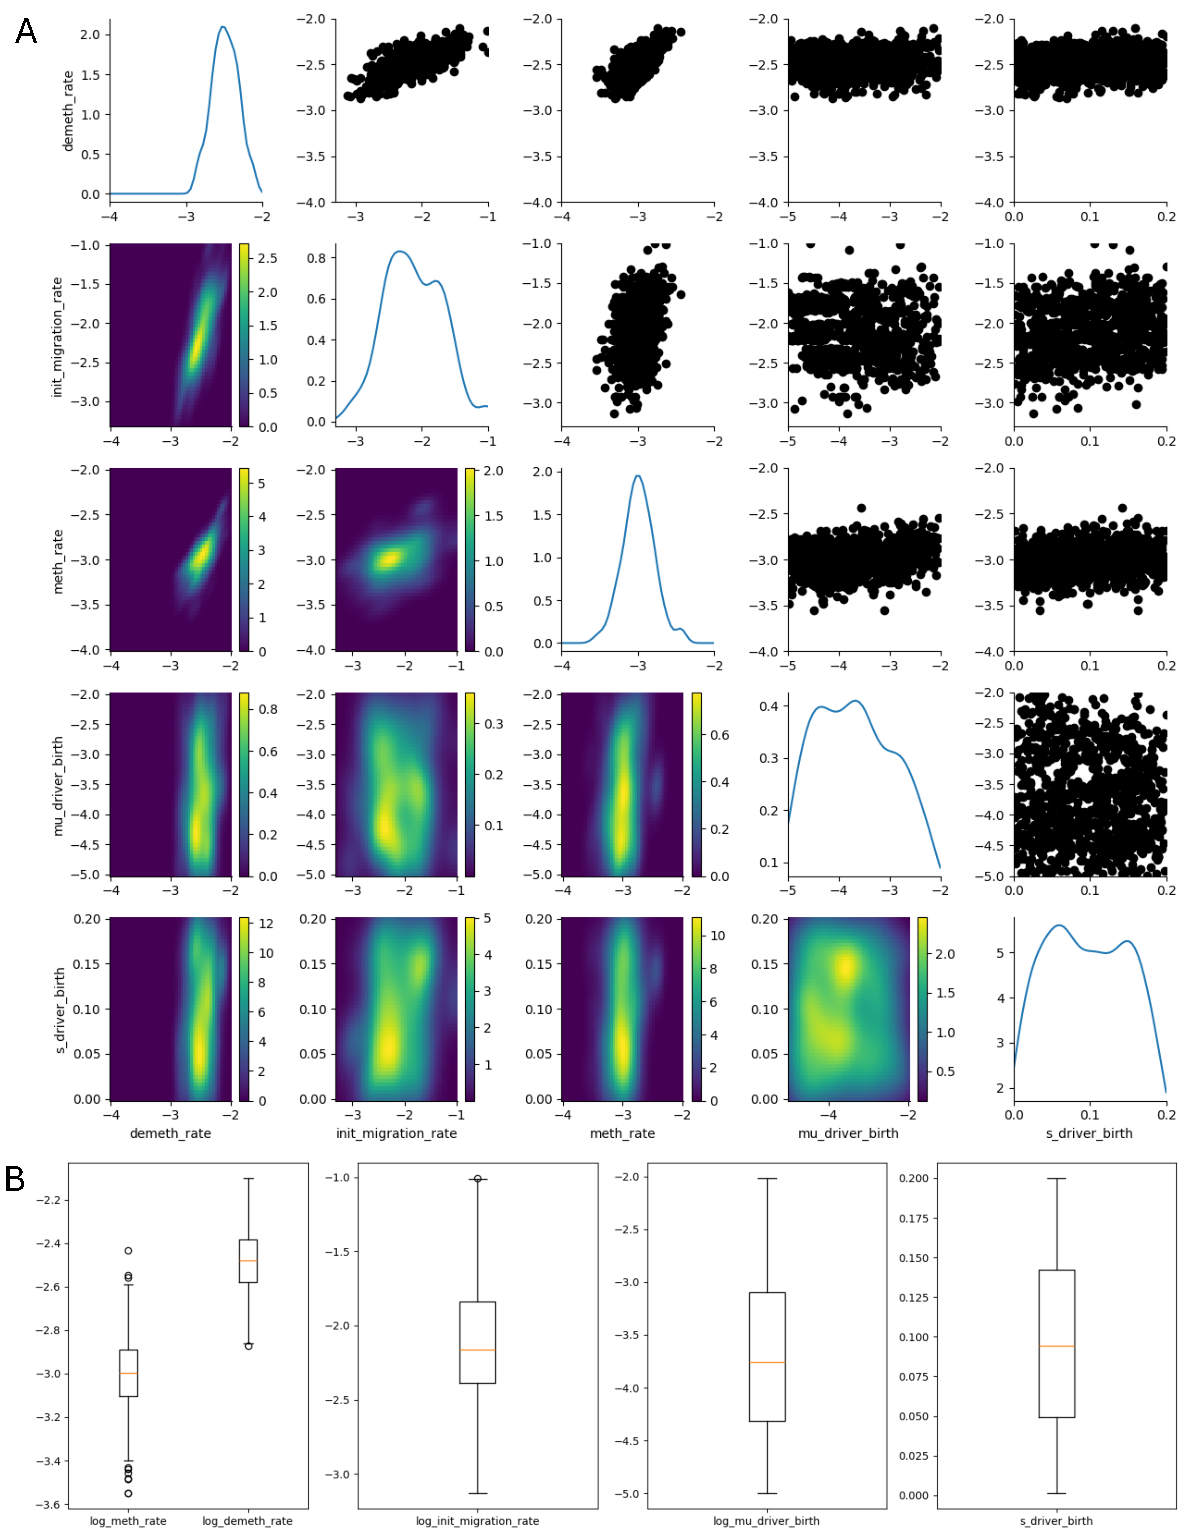
\includegraphics[width=\textwidth]{Chapter_5/figures/inference_raw/inference_2.pdf}
    \caption{Log-transformed parameters lead to more efficient traversal of
    parameter space. \textbf{A} --- posterior distributions of fCpG fluctuation
    rates have narrowed similar to before, but now the fission rate's posterior
    is also narrower than before. Mutation rate and selective advantage are
    still not inferred by the model. \textbf{B} --- box plots of the
    posteriors.}
    \label{fig:inference_2}
\end{figure}
\clearpage

\subsection{Fast- and slow-growing tumours}
The data provided by Dr Shibata contains samples from different patients, with
each tumour being potentially at a different stage of growth. From exploratory
analysis, it seems that some tumours are growing faster than others, if we work
under the assumption that gland fission is the only mechanism of growth. This
hypothesis is supported by the inference results, as samples with higher values
in the inter-gland distance matrix tend to grow slower, and ones where gland
fCpG arrays are more similar have grown faster. The inferred median fission
rates are shown in table \ref{tab:fission_rates}.

\begin{table}[ht]
    \centering
    \begin{tabularx}{\textwidth}{|c|X|X|c|c|}
    \hline
    Tumour & Inferred median fission rate $[\text{cell}^{-1}\text{cell div}^{-1}]$ & $L_2$ half-norm & Tumour size [cm] & Stage \\
    \hline
    I & $0.017$ & 0.176 & 3.6 & III \\
    \hline
    J & $0.003444$ & 0.421 & 5 & III \\
    \hline
    S & $0.007$ & 0.295 & 6 & n/a \\
    \hline
    \end{tabularx}
    \caption{Inferred median fission rates for different tumours and their
    sizes. \textbf{NOTE:} Still running a few more samples on the cluster, will
    update the table with more results when they are done.}
    \label{tab:fission_rates}
\end{table}

As the inferred fission rates from table \ref{tab:fission_rates} are set per
cell per cell division, the fission rate per gland would be $100$ times higher,
or roughly in the interval $(0.1, 1)$ --- one order of magnitude less, or about
the same as the stem cell division rate. In my model, the tumour grows as a pure
birth branching process, meaning that the growth is exponential. Let $\phi$ be
the fission rate and $N(t)$ the number of glands in the tumour at time $t$. Then
\begin{equation}
    N(t) = e^{\phi t}N(0).
\end{equation}
As the tumour grows from a single gland, the time $\tau$ to reach a certain
size $N_\tau$ is
\begin{equation}
    \tau = \frac{1}{\phi}\log N.
\end{equation}
The literature does not provide clear estimates for cancer stem cell division
rates, but I think a reasonable estimate would be from about $1$ per month to
$1$ per week, or about $0.034$ to $0.1$ per day. This would mean that the time
to reach a size of $10^7$ glands would lie in the interval $(230, 7000)$ days,
or about $8$ months to $20$ years. This range is broad, and is not meant as a
precise estimate, but rather a sanity check of the model's outputs. Considering
that the orders of magnitude are correct, the model seems to be able to describe
the observed data well.

\section{Discussion}
% \begin{itemize}
%     \item $1$D model recaps FMC patterns in CRC
%     \item colorectal cancer fcpg data can be explained by effectively neutral
%         evolutionary regimes
%     \item further work - likelihood-based inference, large scale modelling of
%         colorectal cancer
%     \item initial conditions - does a fully random initial array make sense in
%         the context of patterns in data? some tumours do indeed look like they
%         simply have unequal meth and demeth rates, but others look like they
%         started hypo- or hypermethylated.
% \end{itemize}

In this chapter, I tested the \texttt{methdemon} model on colorectal cancer
methylation data using approximate Bayesian computation. The model was able to
recapitulate the patterns observed in the data, and the inferred parameters lay
within reasonable ranges. However, the model struggled to infer the selection
coefficient and the driver mutation rate. This could be due to the signature of
selection being too weak in the model or data, or the distance functions in the
ABC rejection step not being fine-grained enough to detect the differences
between evolutionary modes. Having said that, the results do support an
effectively neutral evolutionary mode of colorectal cancer growth, with the
effects of selection constrained to within glands. Furthermore, it seems clear
that multi-site sequencing of methylation arrays from solid tumours can be used
to draw inferences about the evolutionary dynamics of the tumour, and warrants
further investigation with a more sophisticated model.


\chapter{Discussion}\label{chapter:discussion}

\section{Summary}
Modelling cancer evolution is difficult. Like with any data-driven approach,
straying too far into general laws may lead to underfitting of
patient-specific data. Focussing too much on the individual, however, makes
overfitting the main issue. As novel sequencing techniques, or at least data
collected using them, become more available, there is an increased emphasis on
multi-pronged approaches \cite{heide_assessment_2021, others}. In my view, a
similar conundrum extends one level of abstraction above this, as focussing
solely on data may lead to missing the proverbial forest. Much like branches of
mathematics grew out of necessity to quantify physical phenomena, so has
mathematical theory informed experiments decades later. I believe a similar
approach is essential in mathematical oncology as well, with robust mathematical
frameworks translating into the laboratory or even clinical trials. A good
example would be adaptive therapy, which has the potential to revolutionise
patient care.\par
In chapter \ref{chapter:trees}, I investigated properties of the universal tree
balance index $J^1$. Originally introduced to analyse cancer phylogenies, I show
that the roots of the idea for such a metric go surprisingly deep, with
pioneering works in computer science developing an effectively identical
formula. The expected value of the index under even the simplest tree generation
processes was too complex for me to calculate analytically, so I relied on the
relationship derived in the original $J^1$ paper \cite{lemant_robust_2022} which
connects it with the Sackin index to obtain an accurate approximation. Another
challenge came from deriving tree families which minimise the index. While I
proved that there exists a family of trees on which the value of $J^1$ is lower
than on the caterpillar tree, traditionally the tree that minimises balance
indices, I could only conjecture that this family indeed minimises the index
across all trees on a given number of leaves. \par
Balance is only one property of many trees posses. This meant that the next
logical step was to consider the values of a set of indices during a tree
generating process. Inspired by \cite{noble_spatial_2022}, I used a modified set
of evolutionary indices on the outputs of an agent-based model to test how well
one can distinguish different evolutionary trajectories in the space described
by the indices. These results I compared to a new set of tree shape indices
\cite{noble_new_2023}, which generalise $J^1$ further on trees with defined
branch lengths. NOTE: FINISH THIS. \par
In chapter \ref{chapter:methdemon}, I narrowed down my consideration of the
modes of tumour evolution to the specific case of effectively neutral evolution,
which manifests itself via progressive differentiation. The model I developed in
this chapter restricts the effects of selection to patches of cells, with the
patches themselves not interacting or interacting neutrally. I demonstrated that
ABC could be employed to recover parameters of the model with varying degrees of
accuracy. \par
Having established a workflow inspired by a concrete data set, in chapter
\ref{chapter:methylation} I recovered aspects of evolutionary dynamics of
colorectal cancer using its methylation array data. Building on prior work on
fluctuating methylation clocks, I modelled multi-site bulk sequences of tumour
glands. By considering the differences between spatially close and distant
glands, as well as individual gland fCpG arrays, I was able to approximate the
epimutation and gland fission rates relative to cancer stem cell division rates.
By inferring the rate of tumour growth, it may be possible to more accurately
estimate the age of individual tumours in future studies.

\section{Combining ABM with deterministic models}
\begin{itemize}
    \item ABM allows for study of cell-level dynamics, making it invaluable for
    examining the early stages of cancer evolution, but is not practical at
    whole-tumour scale
    \item cancer, broadly, follows certain deterministic growth laws, but the
    equations fall apart early on or even when just observing individual
    patients
    \item combining the two approaches could allow for a more accurate
    multi-scale model, such as \texttt{methdemon} which leverages coarse-grained
    approximations globally, and ABM locally
\end{itemize}

\section{Hybrid inference approach}
ABM is a powerful tool for studying the evolutionary dynamics of cancer, but the
stochastic nature of small-scale events can make it difficult to obtain results
which are closely aligned with the data, and \texttt{methdemon} is no exception.
Prior work in fCpG modelling was done using a likelihood-based approach
\cite{gabbutt_fluctuating_2022, gabbutt_evolutionary_2023}, and has shown
promising results. Due to the complexity of colorectal cancer, an exclusively
likelihood-based approach may not be feasible, but a hybrid model which
leverages likelihood-based inference locally for detecting potentially small
effects of selection, with ABC on the global scale could be a good compromise.
The main hurdle in this approach is reconciling fissions with the steady-state
turnover process.

\section{Gland phylogenies}
Another piece of the colon cancer fCpG puzzle is the reconstruction of gland
phylogenetic trees. In \cite{gabbutt_evolutionary_2023}, the authors used a custom BEAST pipeline,
a Bayesian phylogenetic inference tool \cite{bouckaert_beast_2019}, to infer
clone phylogenies from blood cancer data. The main differences between the two
data sets include the fact that the blood cancer data is non-spatial, and
therefore possible for meaningful sequencing at multiple points in time. In the
case of colorectal cancer, it is not possible to obtain multiple samples from
the same gland over time. Further, the spatial nature of the data means that
sequencing it in the first place may not be possible before the tumour has been
removed. This means that the clock rate of the gland phylogenies is unknown.
However, sequencing multiple glands does allow for accurate reconstruction of
tree topologies, with the clock rate being a nuisance parameter. Having
discussed the potential for tree shape indices being used in evolutionary mode
inference, the next logical step would be testing whether they point to signs of
global selective pressures in the data. Because of the way \texttt{methdemon} is
written, phylogenies are easily constructed as a byproduct of the simulation,
making it easy to test effectively neutral growth as a null model. Resources
permitting, it would be interesting to use a larger-scale spatial model to test
different ways of gland organisation in space, which could result in different
modes of evolution, and thus tree shapes.

\section{Conclusion}


%Appendices
\appendix
\chapter{Trajectories}\label{app:trajs}

\begin{table}[h]
\centering
\begin{tabularx}{0.75\textwidth}{|X|X|}
\hline
Parameter & Values \\
\hline
    Deme carrying capacity & $1, 512, 8192, \infty$ \\
    Driver mutation rate & $10^{-6}, 10^{-5}, 10^{-4}$ \\
    Selection coefficient & $0.05, 0.1, 0.2$ \\
    Baseline death rate (non-spatial) & $0.98$ \\
    Baseline death rate (spatial) & $0$ \\
\hline
\end{tabularx}
\caption{Parameters used for the simulations. The deme carrying capacity is
    varied across spatial configurations (boundary growth, invasive glandular,
    gland fission, non-spatial respectively), while other parameter variations
    are common to all simulations.}
\label{tab:traj_params}
\end{table}

\begin{figure}[h]
\centering
\includegraphics[width=\textwidth]{Chapter_3/figures/gland_time.png}
\caption{All trajectories in time for the new set of indices plotted for gland
    fission with the average trajectories for different sets of indices plotted
    in colour.}
\label{fig:gland_time}
\end{figure}

\begin{figure}[h]
\centering
\includegraphics[width=\textwidth]{Chapter_3/figures/inv-gland_time.png}
\caption{All trajectories in time for the new set of indices plotted for
    invasive glandular evolution with the average trajectories for different
    sets of indices plotted in colour.}
\label{fig:inv-gland_time}
\end{figure}

\begin{figure}[h]
\centering
\includegraphics[width=\textwidth]{Chapter_3/figures/boundary_time.png}
\caption{All trajectories in time for the new set of indices plotted for
    boundary growth with the average trajectories for different
    sets of indices plotted in colour.}
\label{fig:boundary_time}
\end{figure}

\begin{figure}[h]
\centering
\includegraphics[width=\textwidth]{Chapter_3/figures/non-spatial_time.png}
\caption{All trajectories in time for the new set of indices plotted for
    non-spatial tumours with the average trajectories for different
    sets of indices plotted in colour.}
\label{fig:non-spatial_time}
\end{figure}

\begin{figure}[h]
\centering
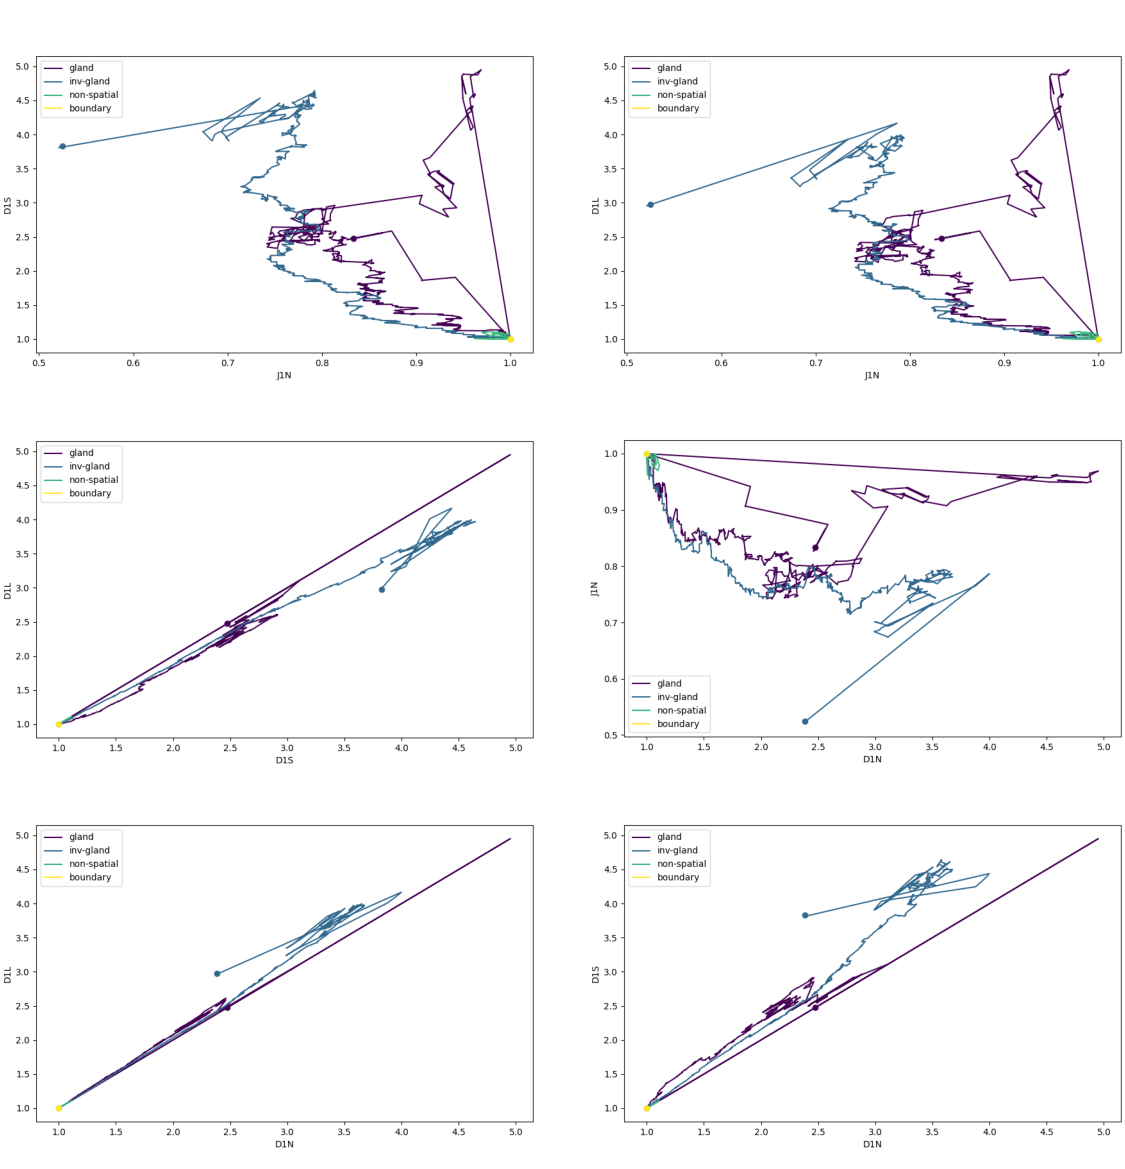
\includegraphics[width=\textwidth]{Chapter_3/figures/1e06005new.pdf}
\caption{Trajectories plotted for the four different spatial configurations for
    the driver mutation rate $\mu=10^{-6}$, and selective coefficient
    $s=0.05$.}
\label{fig:1e06005new}
\end{figure}

\begin{figure}[h]
\centering
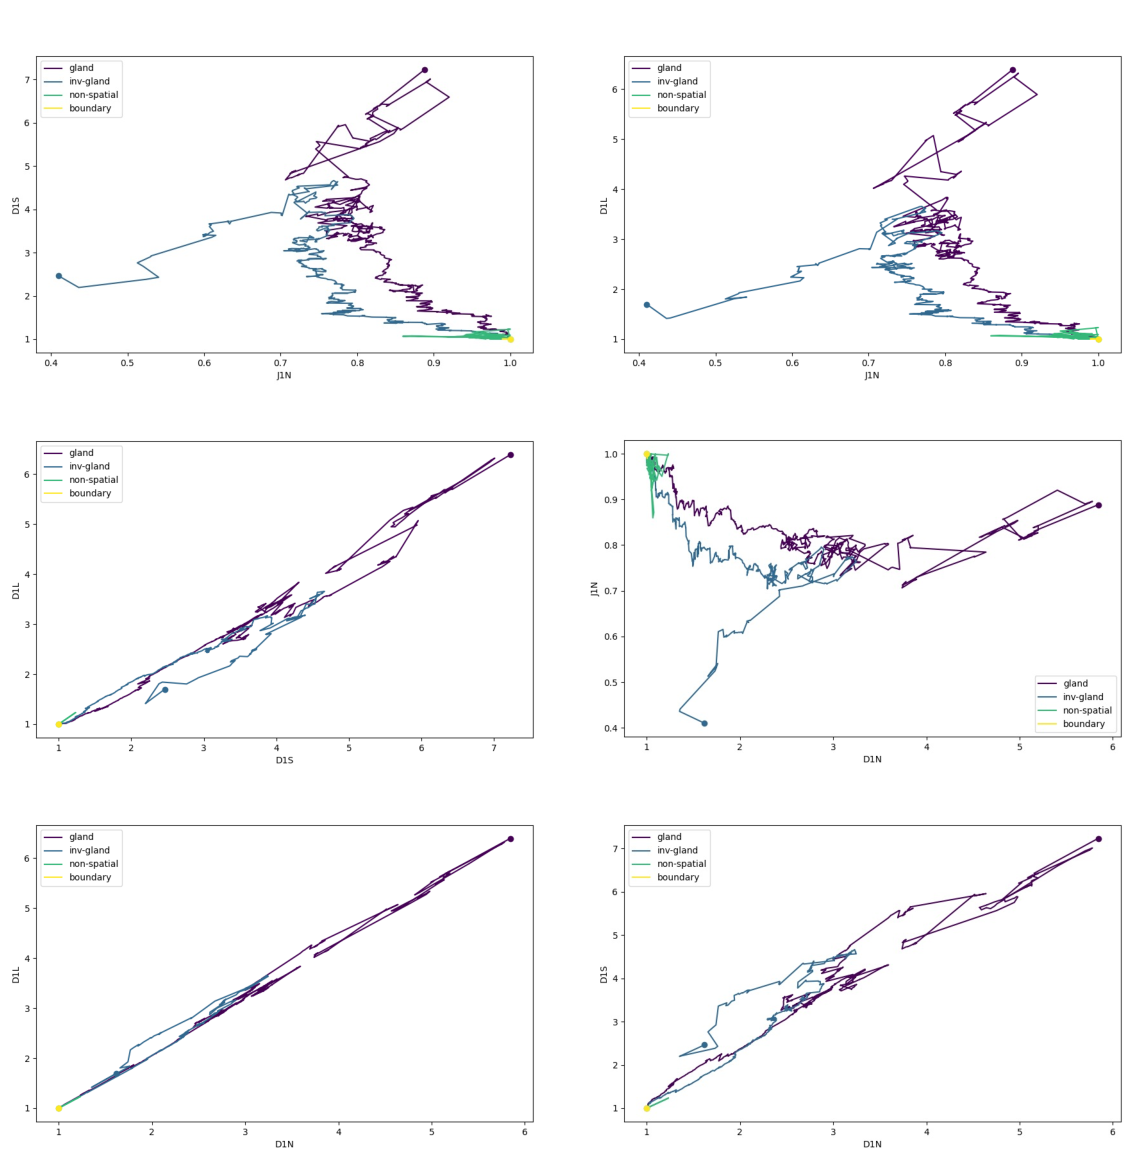
\includegraphics[width=\textwidth]{Chapter_3/figures/1e0601new.pdf}
\caption{Trajectories plotted for the four different spatial configurations for
    the driver mutation rate $\mu=10^{-6}$, and selective coefficient
    $s=0.1$.}
\label{fig:1e0601new}
\end{figure}

\begin{figure}[h]
\centering
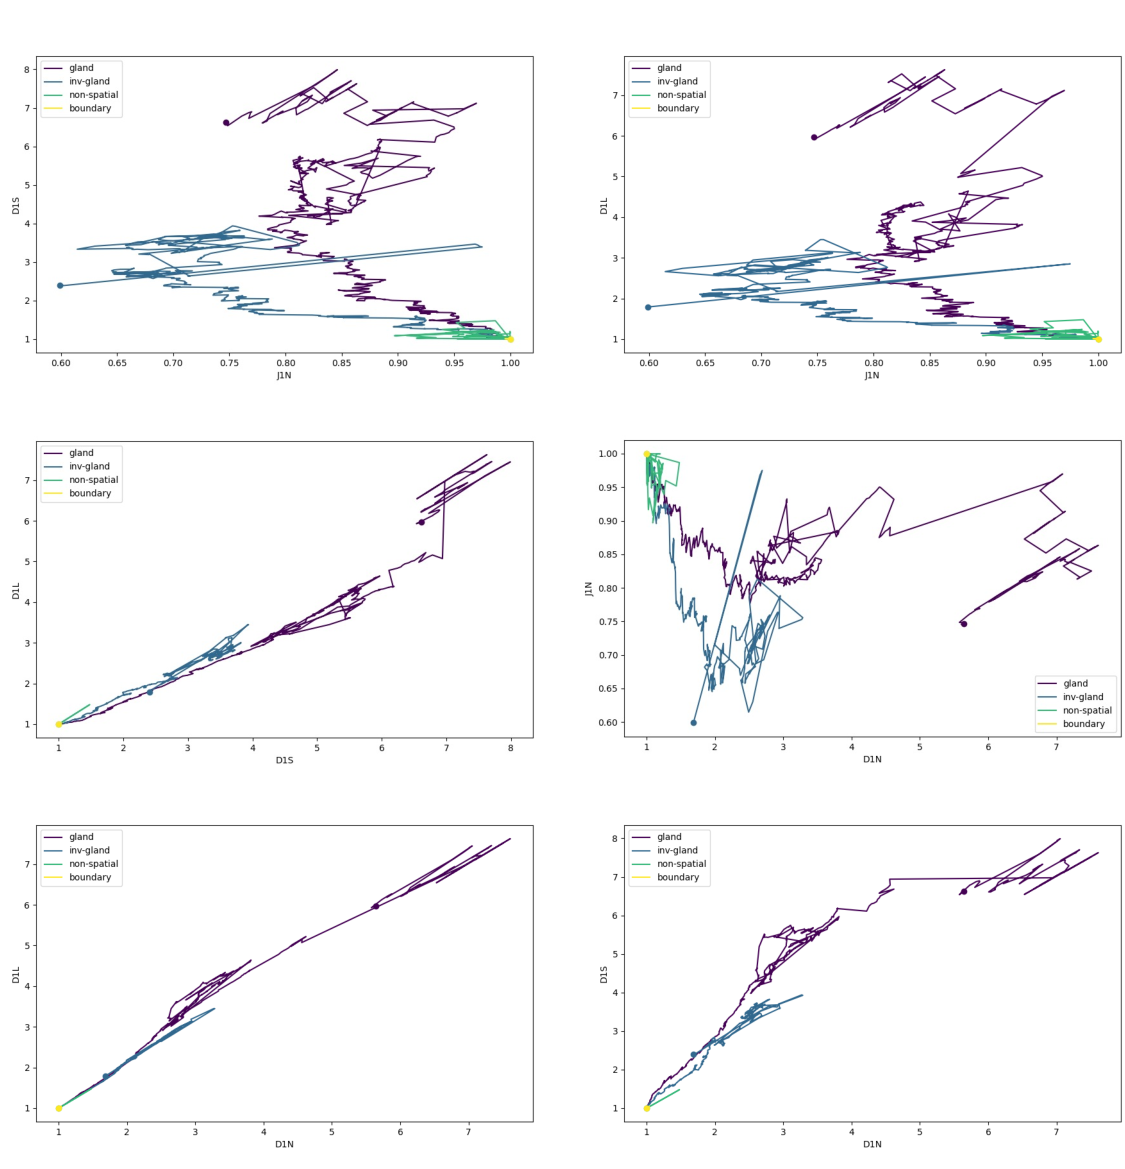
\includegraphics[width=\textwidth]{Chapter_3/figures/1e0602new.pdf}
\caption{Trajectories plotted for the four different spatial configurations for
    the driver mutation rate $\mu=10^{-6}$, and selective coefficient
    $s=0.2$.}
\label{fig:1e0602new}
\end{figure}

\begin{figure}[h]
\centering
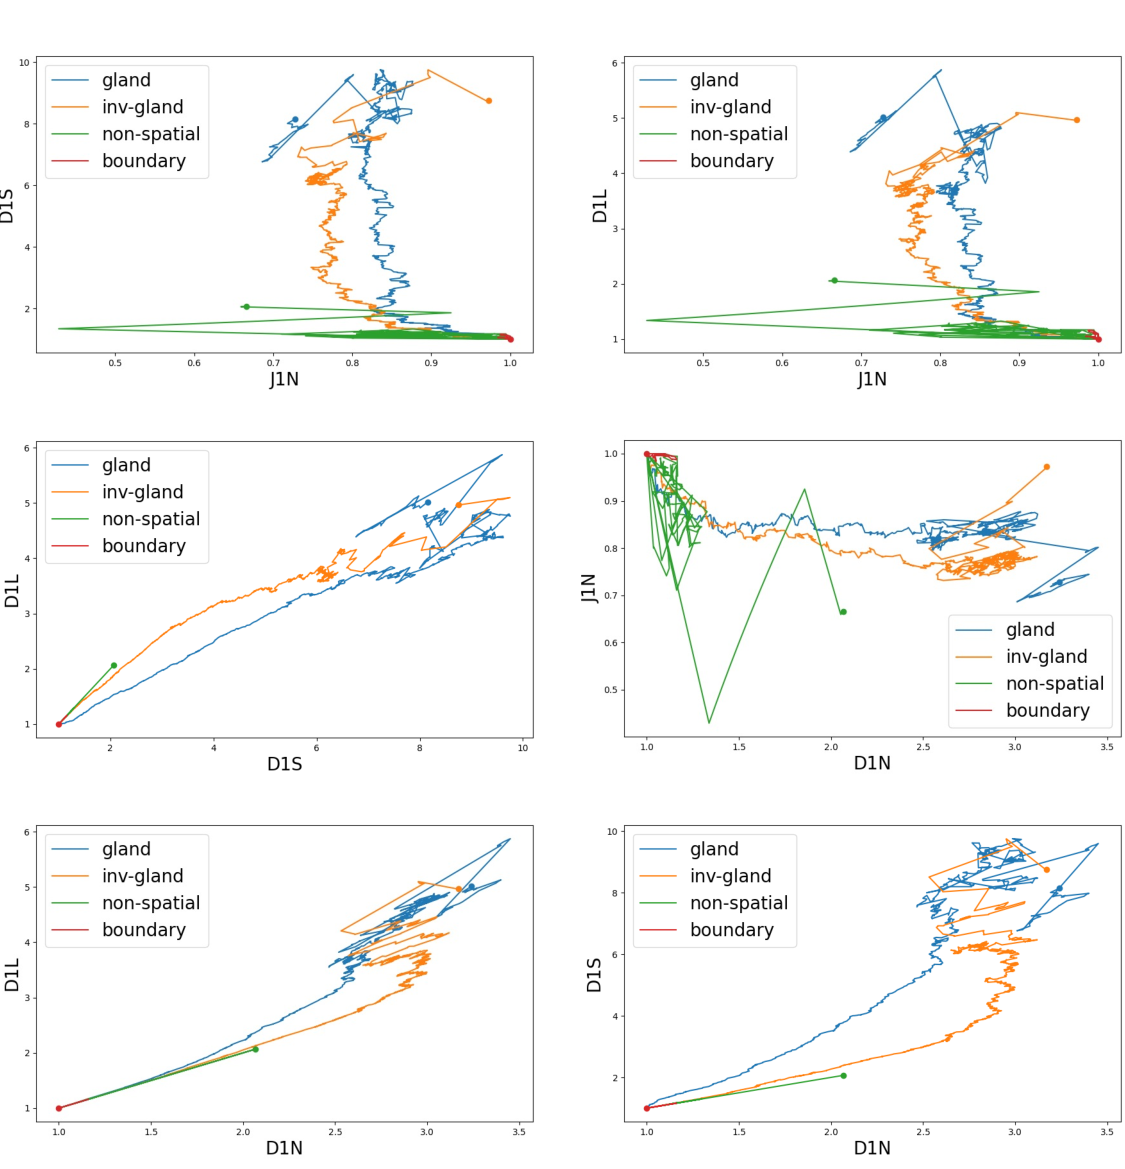
\includegraphics[width=\textwidth]{Chapter_3/figures/1e05005new.pdf}
\caption{Trajectories plotted for the four different spatial configurations for
    the driver mutation rate $\mu=10^{-5}$, and selective coefficient
    $s=0.05$.}
\label{fig:1e05005new}
\end{figure}

\begin{figure}[h]
\centering
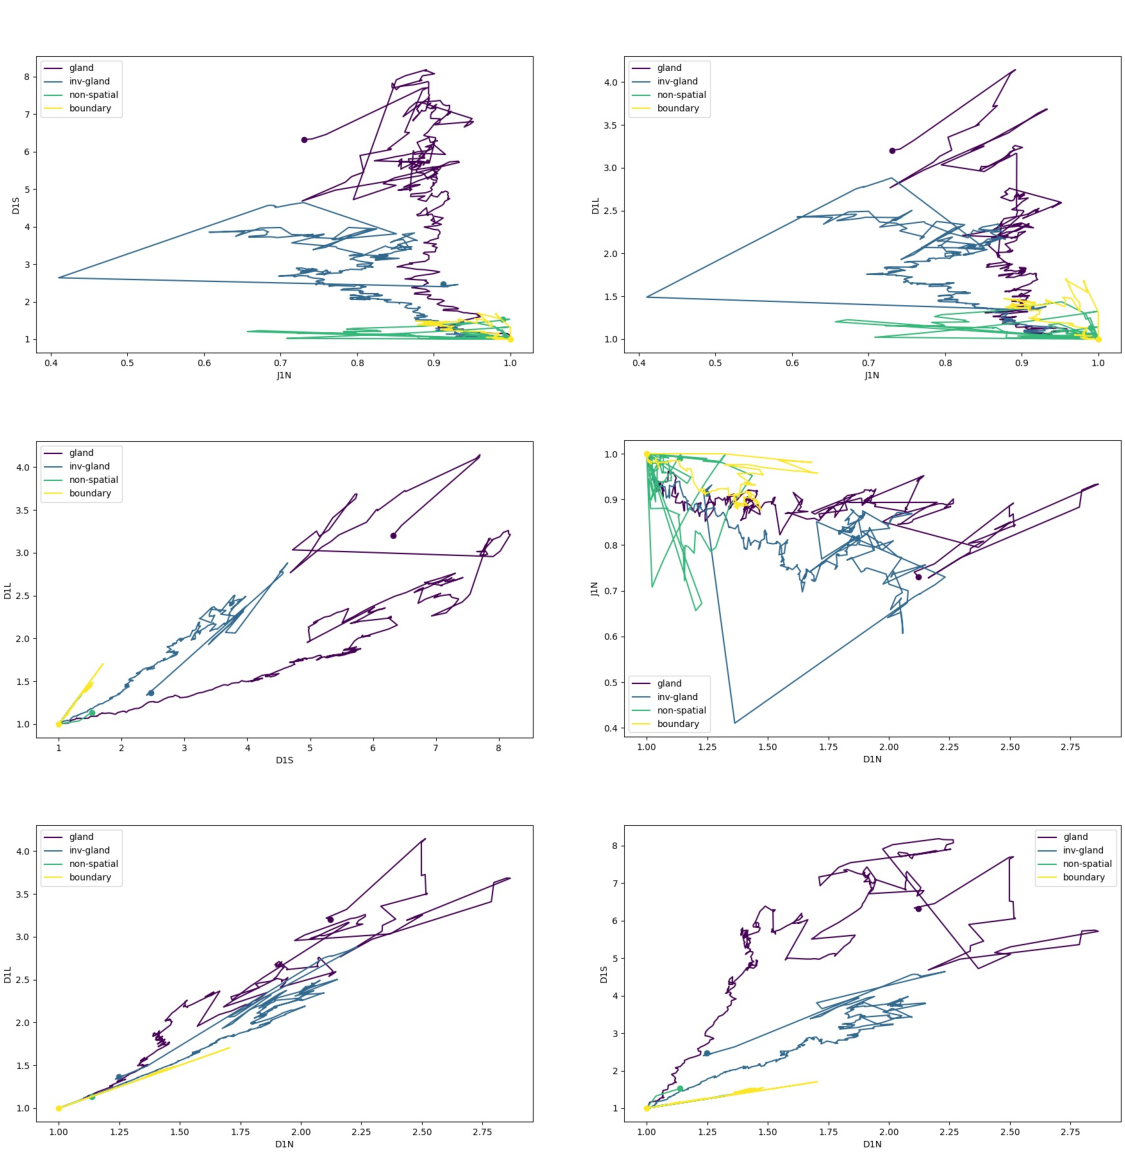
\includegraphics[width=\textwidth]{Chapter_3/figures/1e0502new.pdf}
\caption{Trajectories plotted for the four different spatial configurations for
    the driver mutation rate $\mu=10^{-5}$, and selective coefficient
    $s=0.2$.}
\label{fig:1e0502new}
\end{figure}

\begin{figure}[h]
\centering
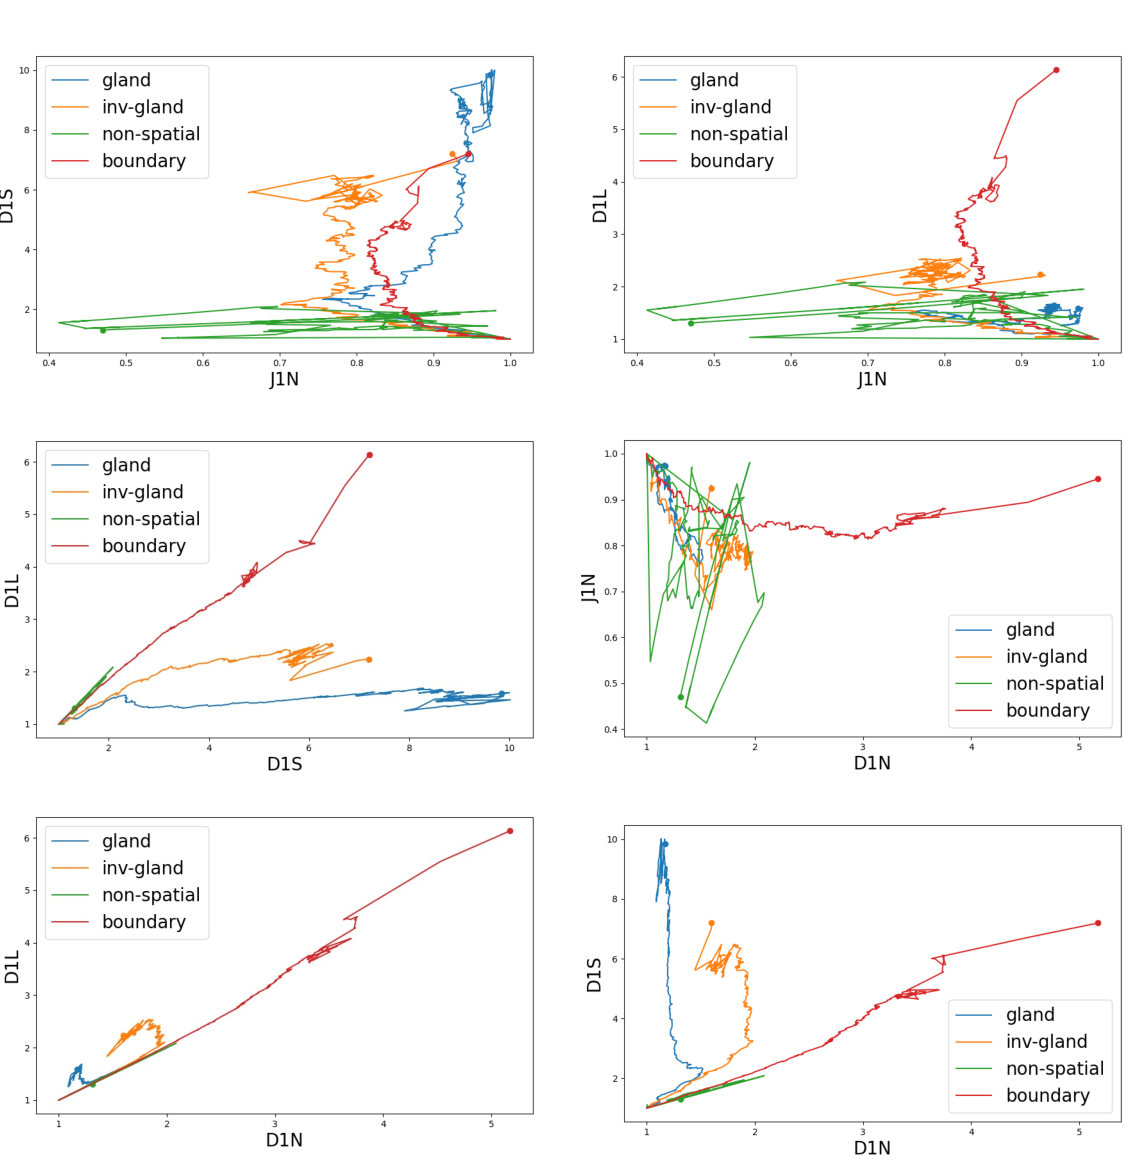
\includegraphics[width=\textwidth]{Chapter_3/figures/1e0401new.pdf}
\caption{Trajectories plotted for the four different spatial configurations for
    the driver mutation rate $\mu=10^{-4}$, and selective coefficient
    $s=0.1$.}
\label{fig:1e0401new}
\end{figure}

\begin{figure}[h]
\centering
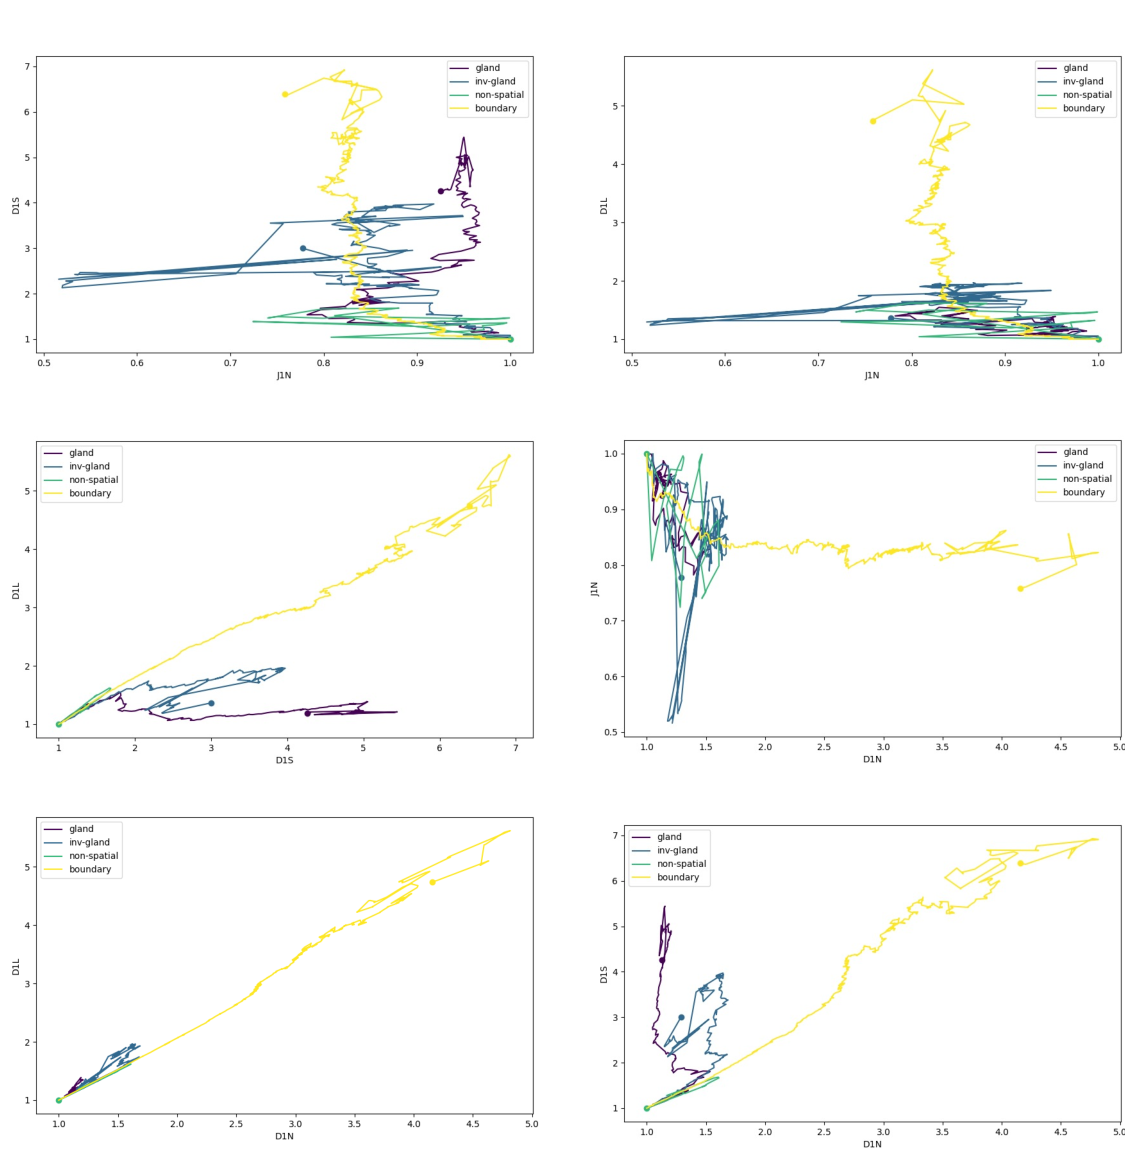
\includegraphics[width=\textwidth]{Chapter_3/figures/1e0402new.pdf}
\caption{Trajectories plotted for the four different spatial configurations for
    the driver mutation rate $\mu=10^{-4}$, and selective coefficient
    $s=0.2$.}
\label{fig:1e0402new}
\end{figure}

\begin{figure}[h!]
    \centering
    \includegraphics[width=\textwidth]{Chapter_3/figures/new_trajs2.png}
    \caption{Individual replicates' index trajectories of boundary growth for
    the parameters used in figure \ref{fig:1e05_01new}. }
    \label{fig:new_trajs2}
\end{figure}

\begin{figure}[h!]
    \centering
    \includegraphics[width=\textwidth]{Chapter_3/figures/new_trajs3.png}
    \caption{Individual replicates' index trajectories of gland fission for the
    parameters used in figure \ref{fig:1e05_01new}. }
    \label{fig:new_trajs3}
\end{figure}

\begin{figure}[h!]
    \centering
    \includegraphics[width=\textwidth]{Chapter_3/figures/new_trajs4.png}
    \caption{Individual replicates' index trajectories of non-spatial growth
    for the parameters used in figure \ref{fig:1e05_01new}. }
    \label{fig:new_trajs4}
\end{figure}





%% Back matter ------------------------------
\backmatter

%Appendices
\chapter{Parameter inference}\label{app:inference}

\begin{table}[h]
\centering
    \begin{tabularx}{0.85\textwidth}{|X|X|X|}
\hline
    Tumour & Median methylation rate & Median demethylation rate \\
\hline
    E & 0.0021 & 0.002  \\
    I & 0.005  & 0.0009 \\
    J & 0.0012 & 0.0018 \\
    S & 0.001  & 0.0033 \\
    X & 0.0008 & 0.0025 \\
\hline
\label{tab:inferred_epimutation_rates}
\end{tabularx}
\caption{Inferred epimutation rates for the tumour samples modelled in this
    thesis.}
\end{table}

\begin{figure}[ht]
\centering
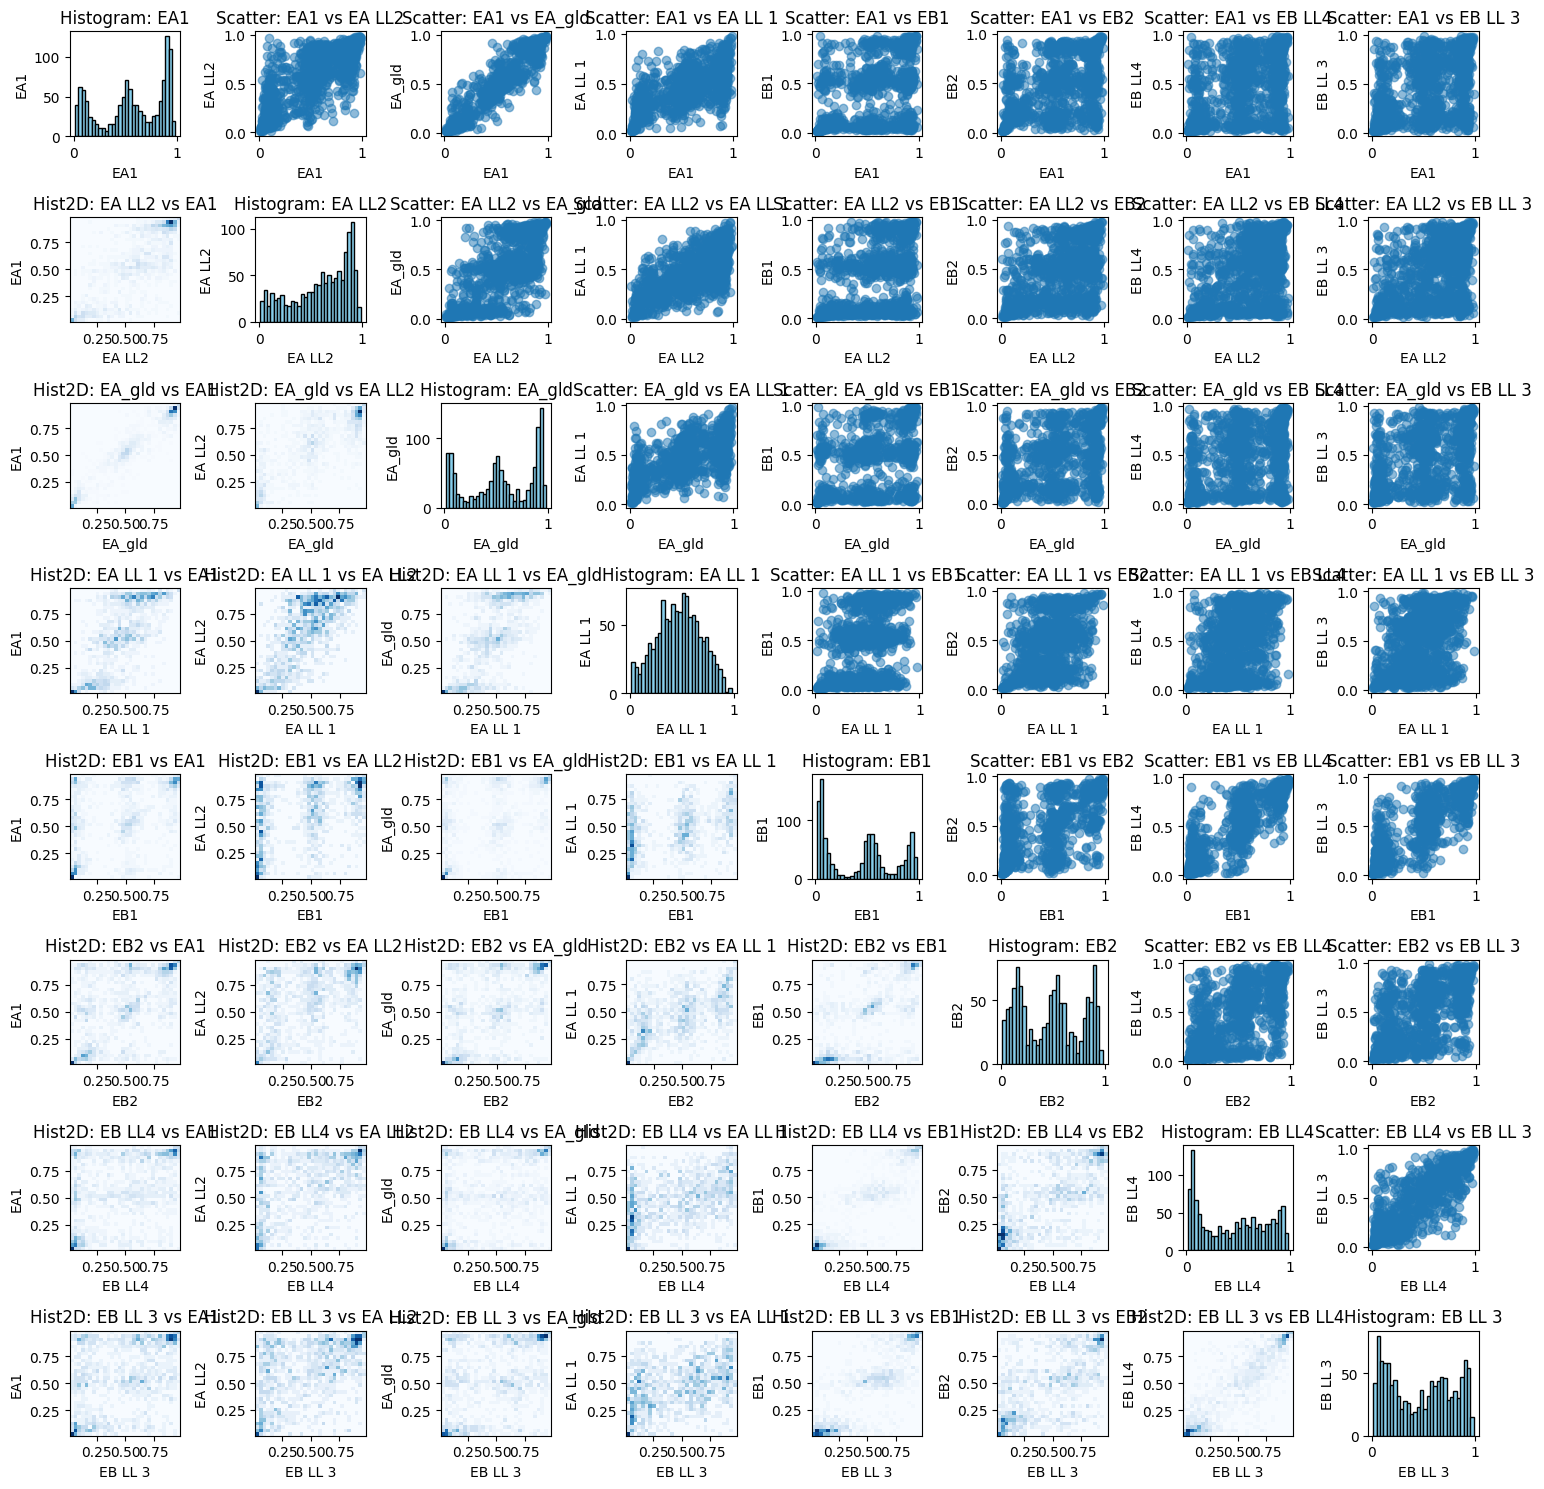
\includegraphics[width=\textwidth]{Chapter_5/figures/fCpG_loci_E.png}
\caption{Visualisation of fCpG arrays for patient E and the inter-gland
    correlation plots.}
\label{fig:vis_E}
\end{figure}

\begin{figure}[ht]
\centering
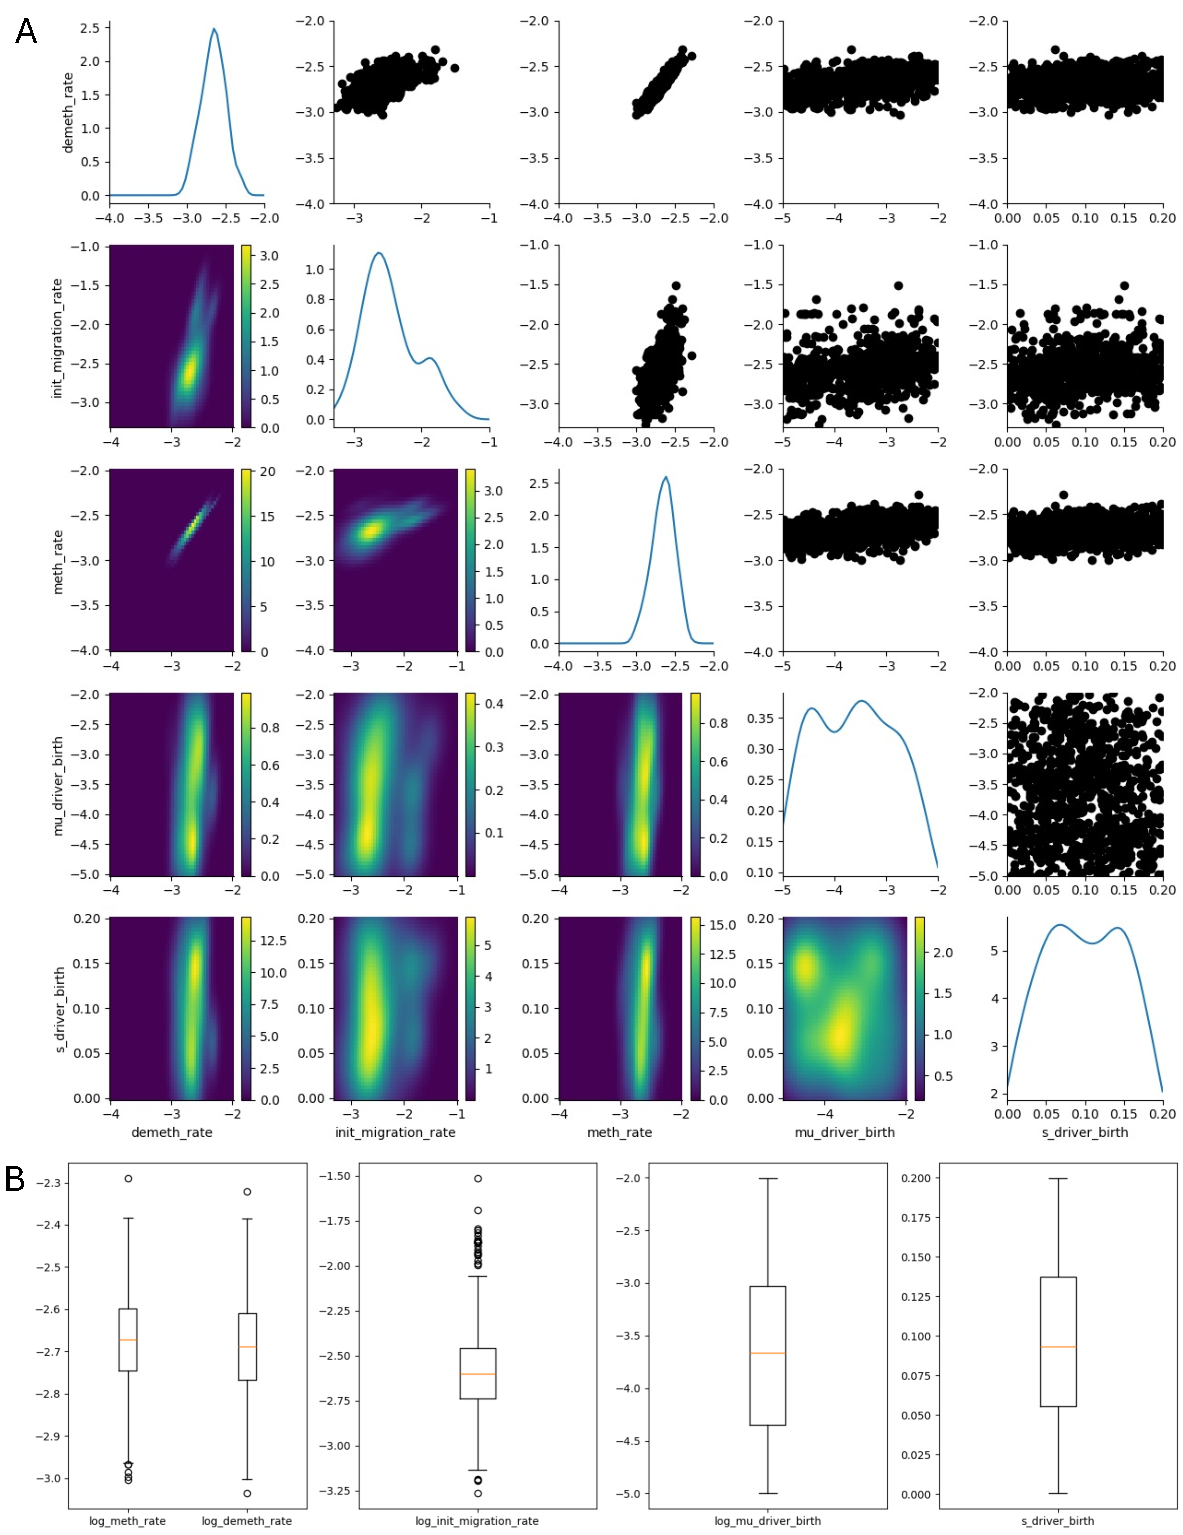
\includegraphics[width=\textwidth]{Chapter_5/figures/inference_E.pdf}
\caption{Parameter inference plots for patient E.}
\label{fig:inference_E}
\end{figure}

\begin{figure}[ht]
\centering
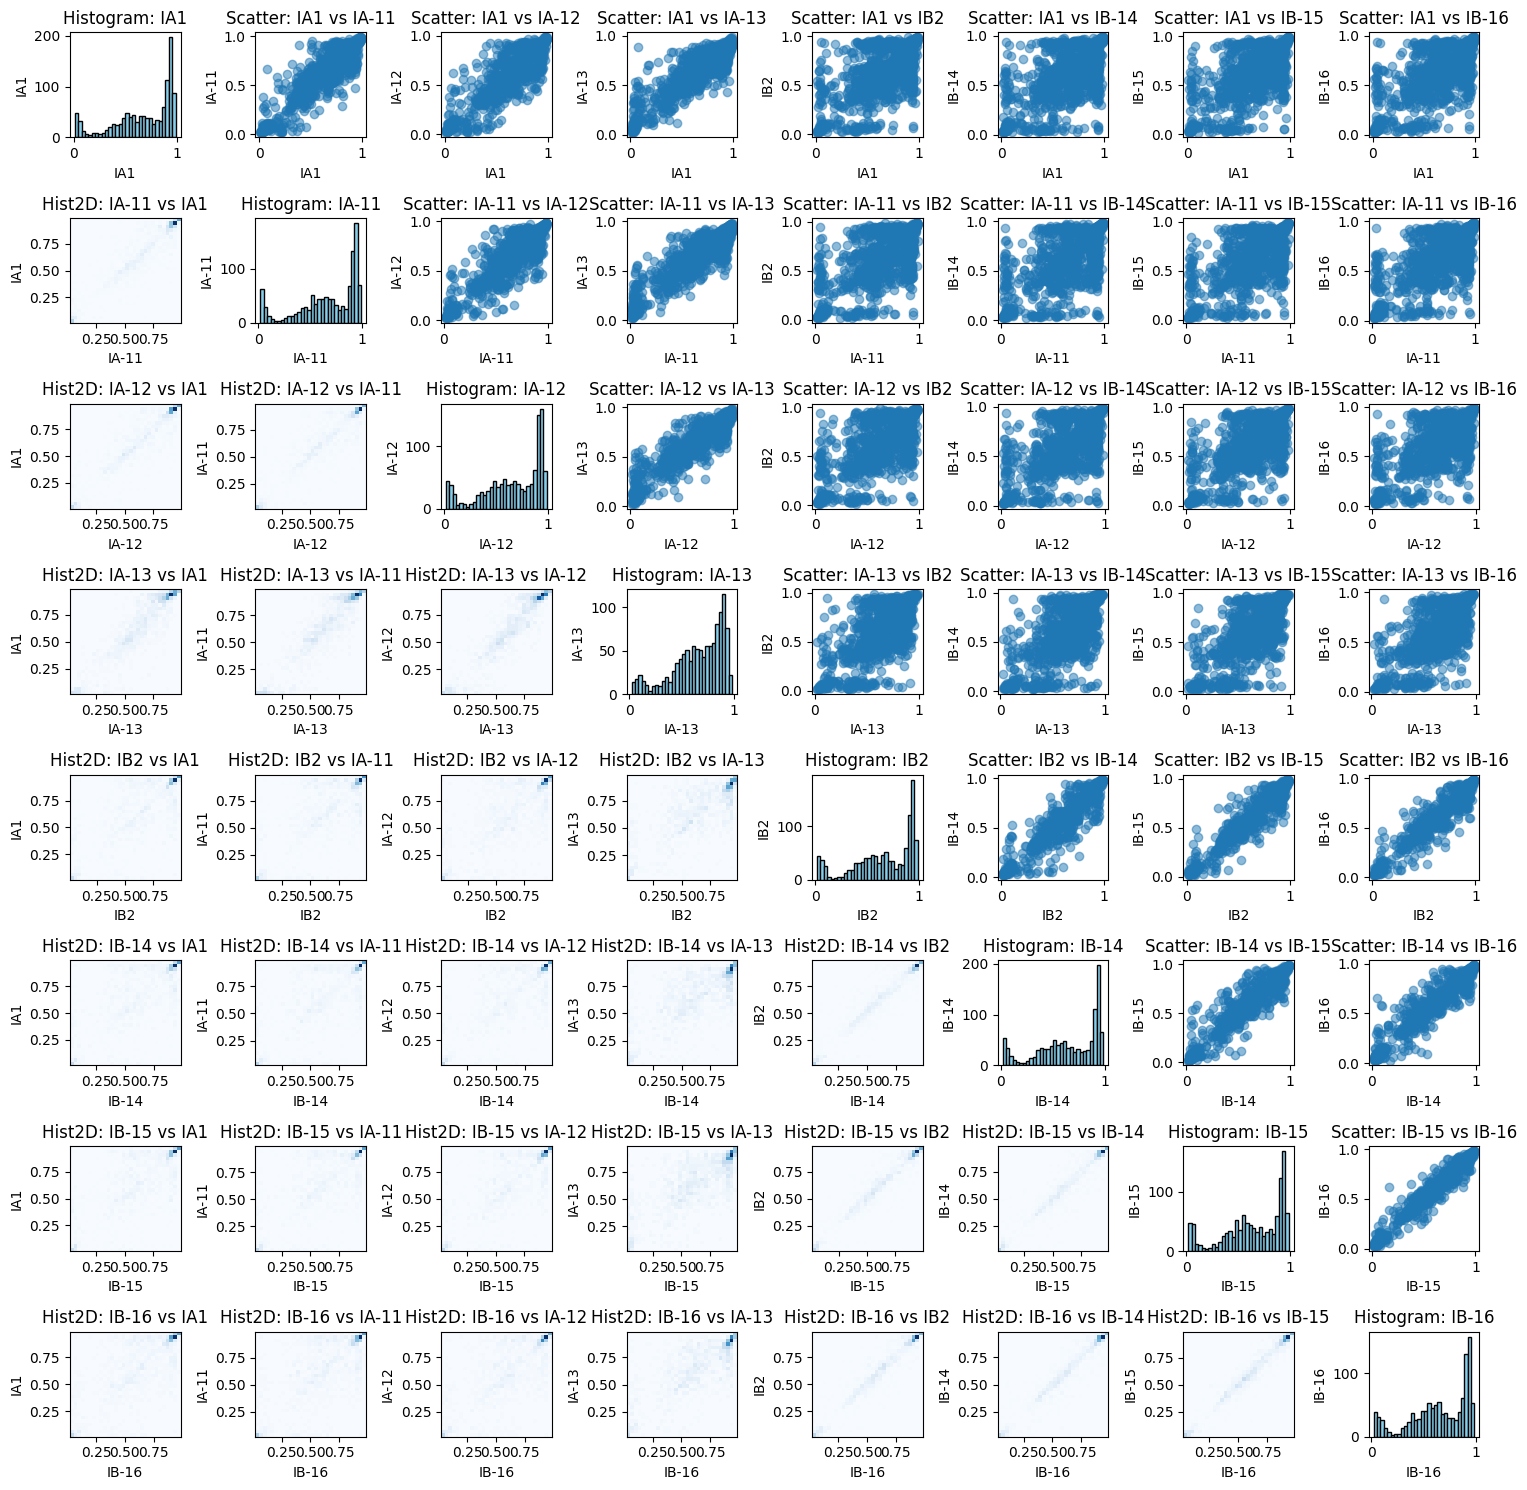
\includegraphics[width=\textwidth]{Chapter_5/figures/fCpG_loci_I.png}
\caption{Visualisation of fCpG arrays for patient I and the inter-gland
    correlation plots.}
\label{fig:vis_I}
\end{figure}

\begin{figure}[h]
\centering
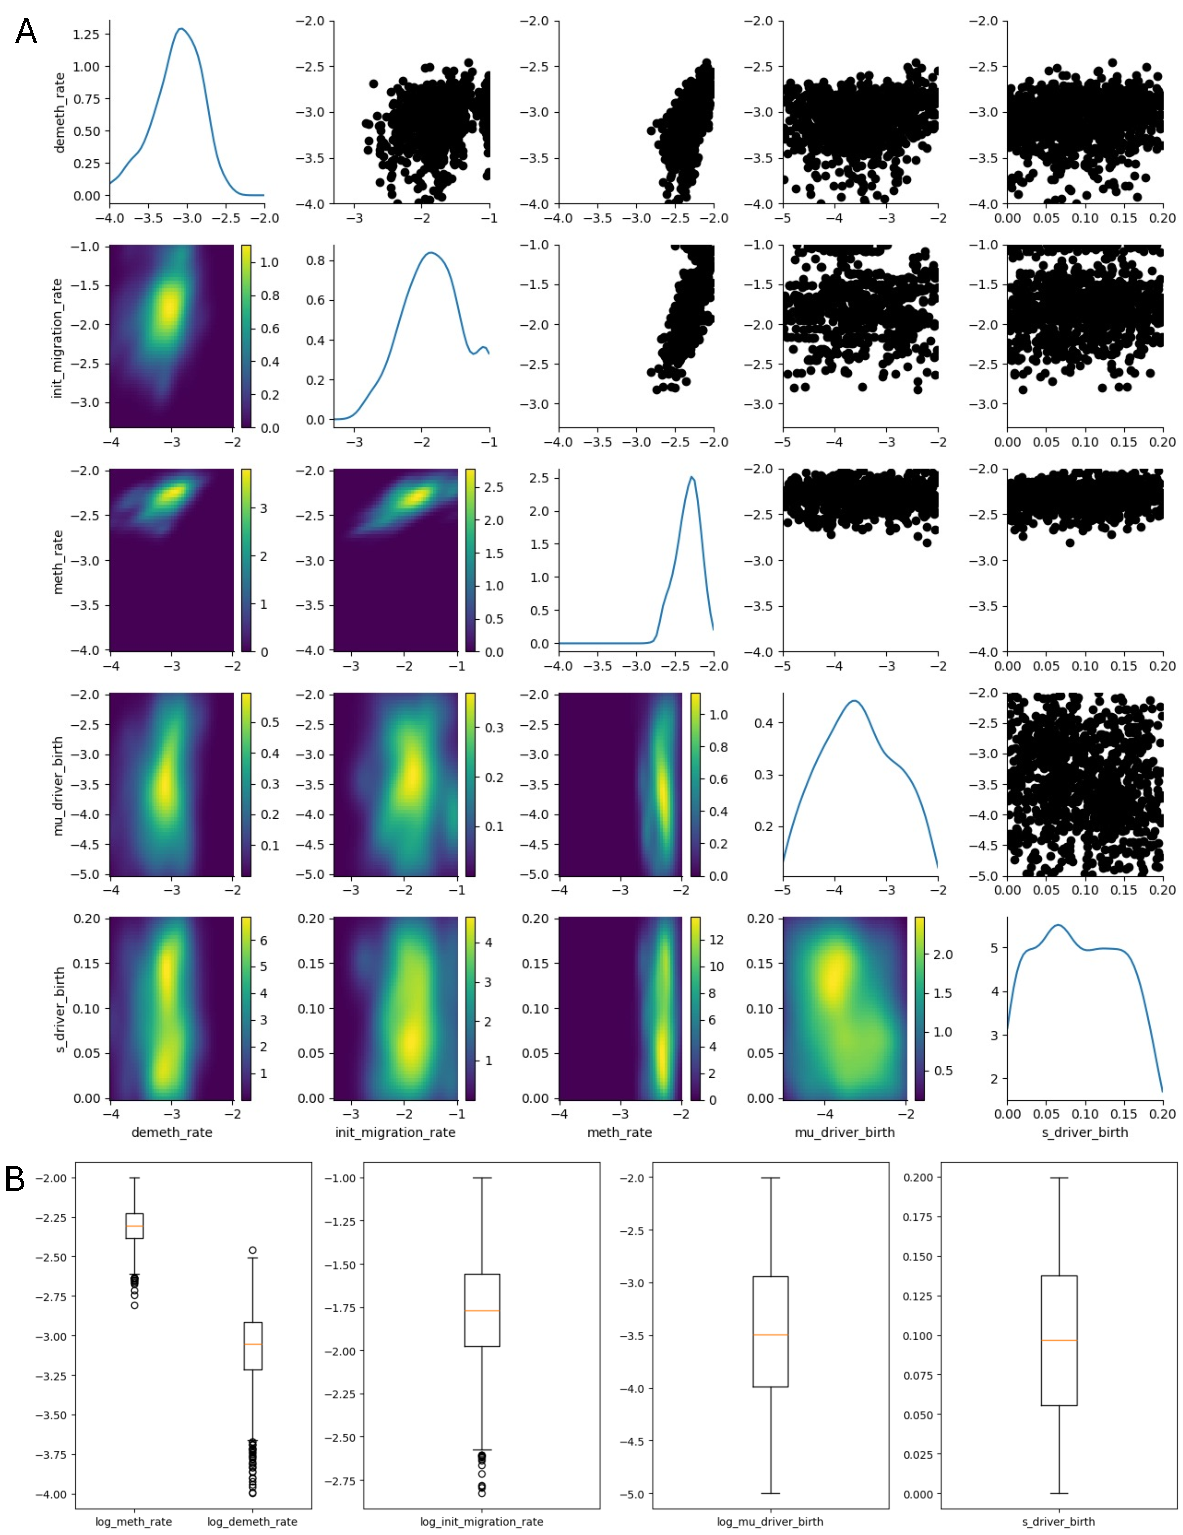
\includegraphics[width=\textwidth]{Chapter_5/figures/inference_I.pdf}
\caption{Parameter inference plots for patient I.}
\label{fig:inference_I}
\end{figure}

\begin{figure}[ht]
\centering
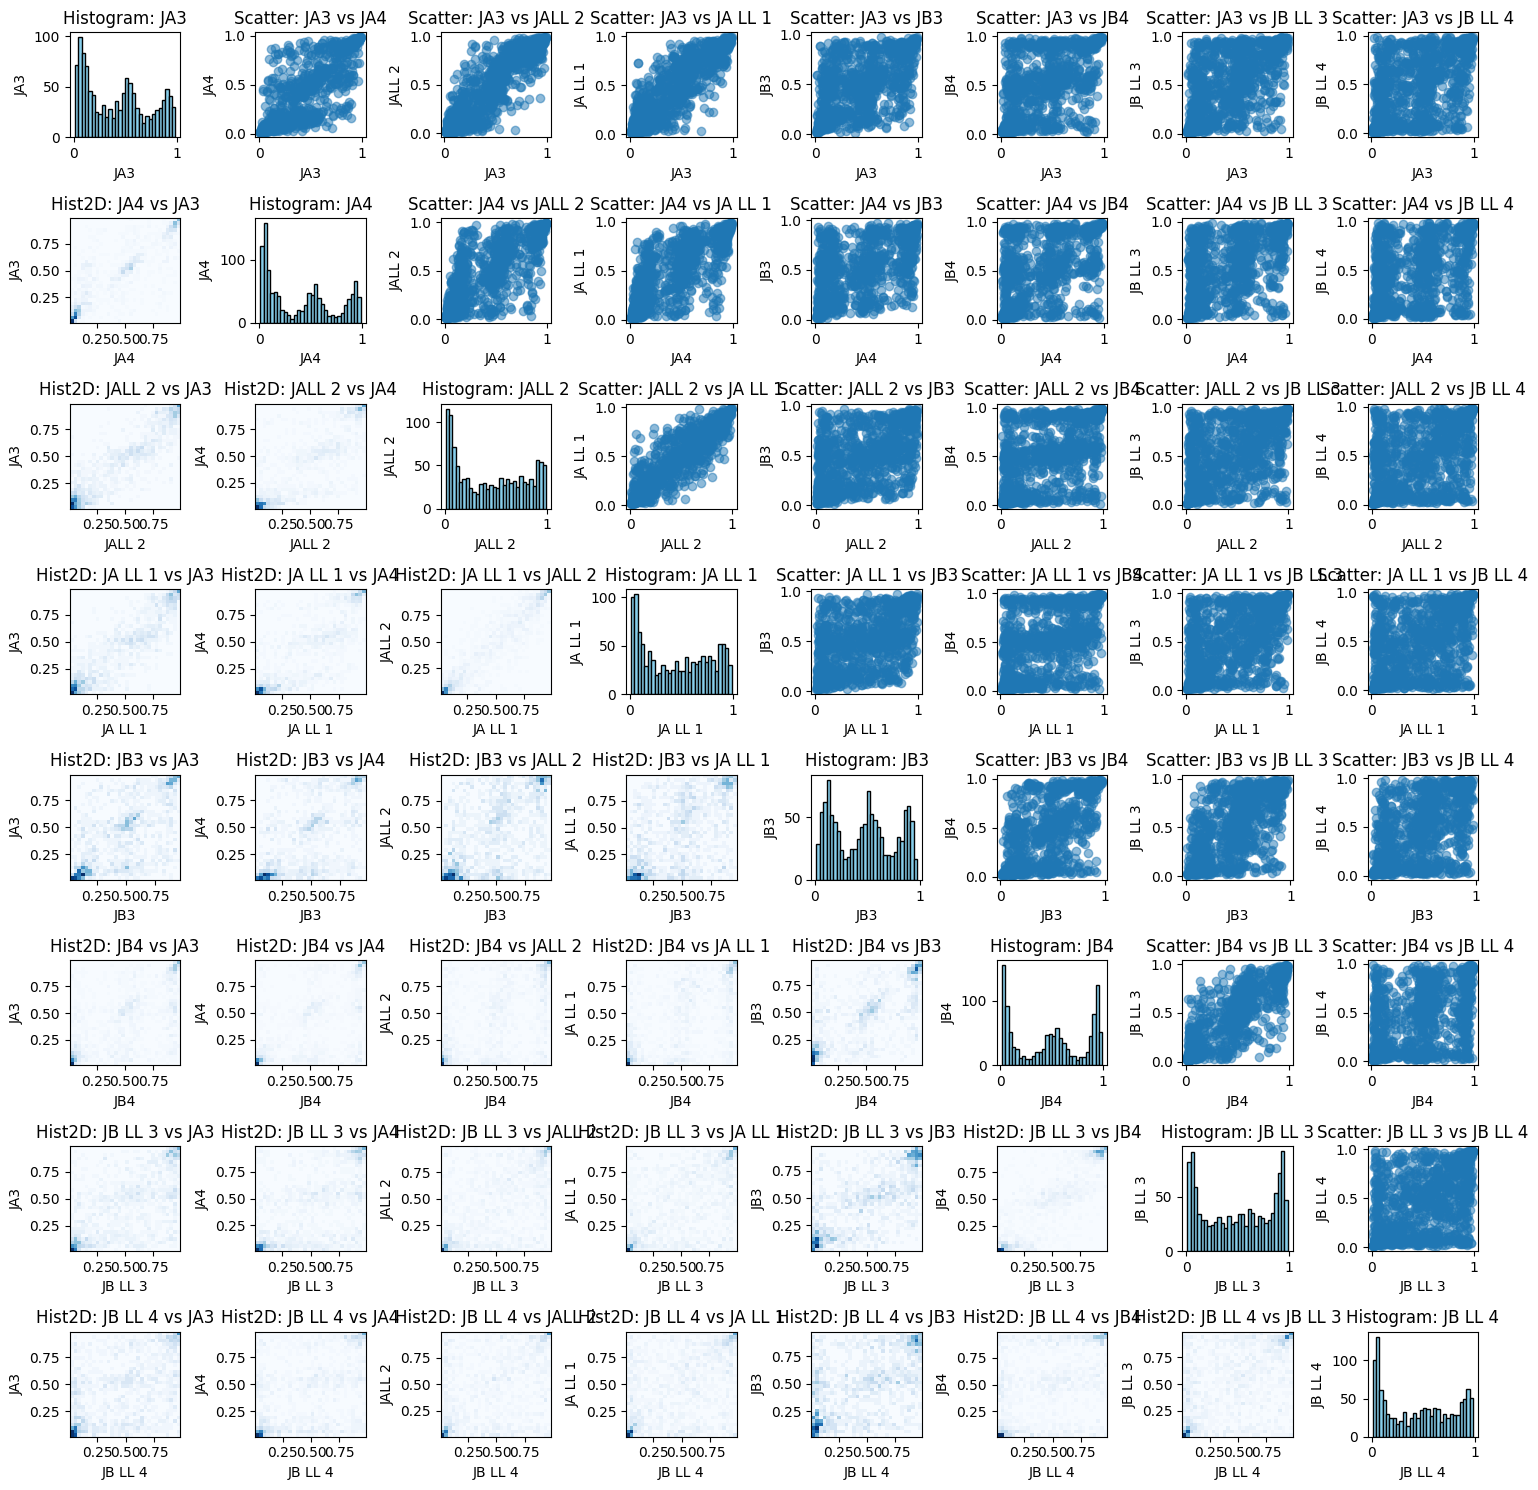
\includegraphics[width=\textwidth]{Chapter_5/figures/fCpG_loci_J.png}
\caption{Visualisation of fCpG arrays for patient J and the inter-gland
    correlation plots.}
\label{fig:vis_J}
\end{figure}

\begin{figure}[h]
\centering
\includegraphics[width=\textwidth]{Chapter_5/figures/inference_J.pdf}
\caption{Inference of the parameters for patient J.}
\label{fig:inference_J}
\end{figure}

\begin{figure}[ht]
\centering
\includegraphics[width=\textwidth]{Chapter_5/figures/fCpG_loci_X.png}
\caption{Visualisation of fCpG arrays for patient X and the inter-gland
    correlation plots.}
\label{fig:vis_X}
\end{figure}

\begin{figure}[h]
\centering
\includegraphics[width=\textwidth]{Chapter_5/figures/inference_X.pdf}
\caption{Inference of the parameters for patient X.}
\label{fig:inference_X}
\end{figure}

\begin{figure}[ht]
\centering
\includegraphics[width=\textwidth]{Chapter_5/figures/gland_dists.pdf}
\caption{Inter-gland distance matrices for the tumours modelled in this thesis.
    Clockwise from top left: E, I, X, J.}
\label{fig:gland_dists}
\end{figure}


%Contributions

%Coment after Contribution title:
\renewcommand{\bibpreamble}{The academic contributions made during the time this research was carried
out are listed below:}

\nocitectb{*}

\cleardoublepage
\phantomsection
\addcontentsline{toc}{chapter}{Contributions}
\bibliographystylectb{agsm}
\bibliographyctb{Bibliography/bbl_user}


%'multibib' package is used to generate the Contribution chapter as an extra bibliography chapter. When using multibib package on Windows it may fail. The solution is to run manually the following compilations:
%pdflatex Thesis.tex
%bibtex Thesis.tex
%bibtex ctb.aux	-> This file is created in the main folder after running the 'bibtex Thesis.tex' compilation.
%pdflatex thesis.tex
%pdflatex thesis.tex
%Check multibib documentation for more options. - https://www.ctan.org/pkg/multibib



%Bibliography
\renewcommand{\bibpreamble}{ } %No coments after bibliography title. It had been changed in Contributions.
\cleardoublepage
\phantomsection
\addcontentsline{toc}{chapter}{Bibliography}
\bibliographystyle{agsm}
\bibliography{Bibliography/zotero.bib}

\end{document}
